% Festlegung des Allgemeinen Dokumentenformats
\documentclass[a4paper,12pt,headsepline]{scrartcl}

% Umlaute unter UTF8 nutzen
\usepackage[utf8]{inputenc}

% Variablen
\newcommand{\titleDocument}{DevOps: Implementierung von Continuous Delivery für Container-basierte Anwendungen}
\newcommand{\authorDocument}{Adam Kuffel (204547)}
\newcommand{\subjectDocument}{Master Thesis im Studiengang IT Management}
\newcommand{\keywordsDocument}{CI/CD, DevOps, Docker, Container}



% PDF Dateien einbinden
\usepackage[final]{pdfpages}

% weitere Pakete
% Grafiken aus PNG Dateien einbinden
\usepackage{graphicx}

% Deutsche Sonderzeichen und Silbentrennung nutzen
\usepackage[ngerman]{babel}

% Eurozeichen einbinden
\usepackage[right]{eurosym}

% Zeichenencoding
\usepackage[T1]{fontenc}

\usepackage{lmodern}

% floatende Bilder ermöglichen
%\usepackage{floatflt}

% mehrseitige Tabellen ermöglichen
\usepackage{longtable}

% landscape tables
\usepackage{lscape}

% Multirow tables
\usepackage{multirow}

% 4. Ebene für Überschriften
% https://tex.stackexchange.com/questions/60209/how-to-add-an-extra-level-of-sections-with-headings-below-subsubsection
\usepackage{titlesec}
\setcounter{secnumdepth}{4}
\titleformat{\paragraph}
{\normalfont\normalsize\bfseries}{\theparagraph}{1em}{}
\titlespacing*{\paragraph}
{0pt}{3.25ex plus 1ex minus .2ex}{1.5ex plus .2ex}


% Unterstützung für Schriftarten
%\newcommand{\changefont}[3]{ 
%\fontfamily{#1} \fontseries{#2} \fontshape{#3} \selectfont}

% Packet für Seitenrandabständex und Einstellung für Seitenränder
\usepackage{geometry}
\geometry{left=3.5cm, right=2cm, top=2.5cm, bottom=2cm}

% Paket für Boxen im Text
\usepackage{fancybox}

% bricht lange URLs "schön" um
\usepackage[hyphens,obeyspaces,spaces]{url}

% Paket für Textfarben
% https://en.wikibooks.org/wiki/LaTeX/Colors
\usepackage{color}

% Mathematische Symbole importieren
\usepackage{amssymb}

\usepackage{float}

% auf jeder Seite eine Überschrift (alt, zentriert)
%\pagestyle{headings}

% erzeugt Inhaltsverzeichnis mit Querverweisen zu den Abschnitten (PDF Version)
\usepackage[
bookmarksnumbered,
pdftitle={\titleDocument},
pdfsubject={\subjectDocument},
pdfauthor={\authorDocument},
pdfkeywords={\keywordsDocument},
hyperfootnotes=false]{hyperref}
%\hypersetup{colorlinks, citecolor=red, linkcolor=blue, urlcolor=black}
%\hypersetup{colorlinks, citecolor=black, linkcolor= black, urlcolor=black}

% neue Kopfzeilen mit fancypaket
\usepackage{fancyhdr} %Paket laden
\pagestyle{fancy} %eigener Seitenstil
\fancyhf{} %alle Kopf- und Fußzeilenfelder bereinigen
\fancyhead[L]{\nouppercase{\leftmark}} %Kopfzeile links
\fancyhead[C]{} %zentrierte Kopfzeile
\fancyhead[R]{\thepage} %Kopfzeile rechts
\renewcommand{\headrulewidth}{0.4pt} %obere Trennlinie
%\fancyfoot[C]{\thepage} %Seitennummer
%\renewcommand{\footrulewidth}{0.4pt} %untere Trennlinie

% für Tabellen
\usepackage{array}

% Runde Klammern für Zitate
%\usepackage[numbers,round]{natbib}

% Festlegung Art der Zitierung - Havardmethode: Abkuerzung Autor + Jahr
\bibliographystyle{alphadin}

% Schaltet den zusätzlichen Zwischenraum ab, den LaTeX normalerweise nach einem Satzzeichen einfügt.
%\frenchspacing

% Paket für Zeilenabstand
\usepackage{setspace}

% für Bildbezeichner
\usepackage{capt-of}

% für Stichwortverzeichnis
\usepackage{makeidx}

\definecolor{code_background_color}{rgb}{0.99,0.99,0.99}
\definecolor{code_border_color}{rgb}{0.7,0.7,0.7}
\definecolor{code_comment_color}{RGB}{17,75,16}

% für Listings
% https://en.wikibooks.org/wiki/LaTeX/Source_Code_Listings
\usepackage{listings}
\lstset{
    breaklines=true,
    numbers=left,
    numberstyle=\tiny,
    numbersep=5pt,
    backgroundcolor=\color{code_background_color},
    commentstyle=\color{code_comment_color},
    keywordstyle=\bfseries,
    stringstyle=\ttfamily,
    showstringspaces=false,
    rulecolor=\color{code_border_color},
    basicstyle=\tiny,
    captionpos=b,
    language=bash
}

% Indexerstellung
\makeindex

% Abkürzungsverzeichnis
\usepackage[german]{nomencl}
\usepackage{xcolor}
\let\abbrev\nomenclature

% Abkürzungsverzeichnis LiveTex Version
% Titel des Abkürzungsverzeichnisses
\renewcommand{\nomname}{Abkürzungsverzeichnis}
% Abstand zwischen Abkürzung und Erläuterung
\setlength{\nomlabelwidth}{.25\textwidth}
% Zwischenraum zwischen Abkürzung und Erläuterung mit Punkten
\renewcommand{\nomlabel}[1]{#1 \dotfill}
% Variation des Abstandes der einzelnen Abkürzungen zu einander
\setlength{\nomitemsep}{-\parsep}
% Index mit Abkürzungen erzeugen
\makenomenclature
%\makeglossary

% Abkürzungsverzeichnis TeTEX Version
% \usepackage[german]{nomencl}
% \makenomenclature
% %\makeglossary
% \renewcommand{\nomname}{Abkürzungsverzeichnis}
% \AtBeginDocument{\setlength{\nomlabelwidth}{.25\columnwidth}}
% \renewcommand{\nomlabel}[1]{#1 \dotfill}
% \setlength{\nomitemsep}{-\parsep}

% Optional: Einzelne Zeilen am Anfang einer Seite unterdrücken (Schusterjungen)
% \clubpenalty = 10000
% Optional: Einzelne Zeilen am Ende einer Seite unterdrücken (Hurenkinder)
% \widowpenalty = 10000
% \displaywidowpenalty = 10000

\begin{document}

% Deckblatt einbinden

\includepdf[pages=-]{deckblatt.pdf}

% hier werden die Trennvorschläge inkludiert
\hyphenation{
Produktiv-umgebung
DevOps
}


% Schriftart Helvetica verwenden
%\usepackage{helvet}
%\renewcommand\familydefault{\sfdefault}

% römische Numerierung
\pagenumbering{roman}

% 1.5 facher Zeilenabstand
\onehalfspacing

\newpage

% Einleitung / Abstract
\thispagestyle{empty}
\section*{Zusammenfassung}

Hersteller von Individualsoftware müssen immer schneller und flexibler auf geänderte Anforderungen reagieren können.
Der Begriff DevOps fällt dabei häufig zusammen mit den Begriffen Automatisierung, Infrastructure as Code,
Continuous Delivery und Docker.
Diese Arbeit erklärt die diversen Begriffe anhand der aktuellen Literatur,
untersucht und vergleicht verschiedene \textsl{DevOps-Tools},
um daraus eine exemplarische Implementierung für die technischen Aspekte der Nutzung von DevOps in einem
Software-Unternehmen zu entwickeln.

\section*{Abstract}

Manufacturers of custom software must handle changed requirements faster and more flexible.
The term DevOps is often used in conjunction with the term automation, infrastructure as code, continuous delivery
and Docker.
This thesis will explain the terms based on current literature,
evaluates and compares different \textsl{DevOps-Tools}
to implement an example that will cover the technical aspects of using DevOps in a software company.



% einfacher Zeilenabstand
\singlespacing

\newpage
% Seitenzählung bei Inhaltsverzeichnis beginnen
\setcounter{page}{1}

% Inhaltsverzeichnis anzeigen
\thispagestyle{empty}
\tableofcontents
\newpage
\fancyhead[L]{\nouppercase{\leftmark}} %Kopfzeile links

% 1,5 facher Zeilenabstand
\onehalfspacing

% arabische Seitennummerierung ab hier
\pagenumbering{arabic}

% Einleitung
\fancyhead[L]{\nouppercase{Einleitung}}
\section{Einleitung}\label{einleitung}

Die meisten Unternehmen sind auf eine funktionierende IT angewiesen, selbst wenn diese nicht deren Produkt ist,
sondern als interne Dienstleistung verwendet wird. \footnote{Alt, Auth, Kögler, vgl.~\cite{Alt2017}~[S.217- S.220]} \footnote{Wiedemann, vgl.~\cite{Wiedemann2019}~[S.157]}
Ein Ausfall von IT-Systemen führt i.d.R. direkt oder indirekt zu finanziellen Einbußen.
Wenn die System nur intern verwendet werden, kommt es zunächst zu einem Produktivitätsverlust.
Für Unternehmen deren Produktpalette hauptsächlich softwaregestützte Dienstleistungen sind, entstehen jedoch direkt Umsatzeinbußen. \\

Der reibungslose Betrieb von IT-Systemen ist somit geschäftskritisch. \footnote{Alt, Auth, Kögler, vgl.~\cite{Alt2017}~[S.217- S.220]}
Darüber hinaus stellt die deutlich höhere Innovationsgeschwindigkeit von IT-Systemen enorme Anforderungen an IT-Abteilungen.
Diese müssen immer schneller auf neue Gegebenheiten und Kundenanforderungen reagieren. \\

Insbesondere Unternehmen, deren Hauptprodukt Software ist, haben somit ein gesteigertes finanzielles Interesse an dem reibungslosem Betrieb der IT trotz häufiger Änderungen.
Bekannte Beispiele wie Netflix, Spotify und PayPal haben Dinge aus der \emph{realen} Welt wie Filmverleih, Tonträger und Bargeld in Software umgesetzt.
Unternehmen wie Airbnb oder Uber haben auch dafür gesorgt das die Trennung zwischen der \emph{realen} Welt und IT nicht mehr so einfach differenziert werden kann.
\footnote{Mazzara, vgl.~\cite{Mazzara2019}~[S.100]} \\

Gerade diese Unternehmen haben ihre Branchen verändert und mitunter sogar andere Konkurrenten verdrängt.
Sie haben IT-Innovationen nicht verpasst, sondern es geschafft Treiber dieser Innovationen zu werden.
Wenn Unternehmen längere Zeit IT-Innovationen verpassen, kann ihre Wettbewerbsfähigkeit dadurch gefährdet sein. \footnote{Alt, Auth, Kögler, vgl.~\cite{Alt2017}~[S.217- S.220]} \\

Denn durch die Entwicklungen im Bereich von mobilen Anwendungen, die im Prinzip von jedem veröffentlicht werden können,
laufen Unternehmen Gefahr von einem wesentlich kleineren und schnelleren neuen Anbieter bzw. Startups verdrängt zu werden.
Dabei gewinnt oft nicht derjenige, der die größte Qualität liefert, sondern derjenige der neue Anforderungen schneller umsetzen kann. \\

Um Innovationen umsetzten zu können, müssen Unternehmen ihre IT-Systeme anpassen und verändern können, ohne den Betrieb dabei zu gefährden.
Gerade bei der Entwicklung von Individualsoftware hat sich gezeigt, dass agile Methoden den klassischen Modellen wie z.B. dem Wasserfallmodell überlegen sind.
Dies ist zumindest der Fall, wenn die Anforderungen zu Beginn nicht klar definiert sind oder sich im Laufe der Entwicklung verändern. \\

Der Begriff, der sich im Rahmen von agiler Softwareentwicklung häufig neben Scrum Verwendung findet, lautet DevOps.
Dabei handelt es sich um ein Kunstwort aus den Begriffen Development und Operations somit stellt es keine klar definierte Methode oder Technik. \footnote{Alt, Auth, Kögler, vgl.~\cite{Alt2017}~[S.218]}
So ist DevOps bspw. das Resultat der Anwendung von Prinzipien aus der Herstellung von physischen Gütern bei Toyota \footnote{Kim et. al, vgl.~\cite{Kim2018}~[S.3 - S.4]} \\

Unternehmen wie Facebook, Netflix und Amazon haben hierbei den Trend zu DevOps beschleunigt.
Bereits 2013 hat Facebook wöchentlich neue Versionen ihrer Anwendung direkt in ihren Produktivsystemen installiert und somit zum Kunden gebracht. \footnote{Feitelson, Beck, vgl.~\cite{Feitelson2013}~[S.13]} \\

Eine Studie aus dem Jahr 2019 brachte hervor, dass Unternehmen, die als sogenannte DevOps Leader gelten, im Durchschnitt 208 mal häufiger Software in ihren Produktivsystemen bereitstellen als ihre Mitbewerber.
Der Maximalwert in dieser Umfrage lag hier bei 1460 Deployments im Jahr und der niedrigste Wert bei 7 Deployments im Jahr.
\footnote{https://www.zdnet.com/article/devops-leaders-deliver-software-200-times-more-frequently-than-their-peers-study-shows/, vgl.~\cite{ZDNET_DEVOPS}} \\

Netflix gibt an, tausende Male am Tag Änderungen in die Produktion zu überführen.
Amazon hat während ihrer Umstellung von eigenen Servern auf AWS durchschnittlich alle 11.7 Sekunden neuen Code bereitgestellt.
\footnote{https://techbeacon.com/devops/10-companies-killing-it-devops, vgl.~\cite{TECHBEACON}} \\

Die vorgenannten Beispiele haben viele Unternehmen dazu veranlasst, eigene Strategien im Bereich DevOps und Continuous Delivery zu verfolgen.
\subsection{Problemstellung und Zielsetzung}\label{problemstellung_ziel}

Dem Begriff DevOps werden viele Definitionen zugeordnet.
DevOps beschreibt vor allem eine Philosophie, die von Unternehmen zunächst verstanden und angewendet werden muss.
Die Herausforderungen, die sich dabei ergeben, sind nicht nur technischer Natur und können nicht von einem auf den anderen Tag umgesetzt werden.
Neben den organisatorischen Maßnahmen gibt es darüber hinaus noch technische Fragestellungen, die bei einer \textsl{Umstellung} auf DevOps zu beachten sind.
Diese Arbeit erläutert die verschiedenen Begriffe, welche rund um \textsl{DevOps, Continuous Integration und Continuous Delivery} in der Literatur beschrieben werden. \\

Ziel ist eine Continuous Delivery Pipeline für Docker-Container basierte Anwendungen exemplarisch umzusetzen.
Die Umsetzung soll hierbei die zuvor ermittelten für DevOps relevanten organisatorischen Herausforderungen berücksichtigen
und es Entwicklern ermöglichen, Codeänderungen innerhalb weniger Minuten in einer Produktivumgebung zu installieren. \\

Hierzu werden gängige Tools im Zusammenhang mit Codeverwaltung, Zusammenarbeit der Entwickler, Build Systeme, Infrastructure as Code und Container
as a Service Angebote diverser Cloud Provider untersucht, um daraus einen möglichen Weg für Continuous Delivery zu implementieren.
\subsection{Beschreibung der Anwendung}\label{beschreibung_anwendung}

Die bekanntesten Beispiele für DevOps Leader sind Webanwendungen.
Diese Arbeit wird insbesondere die Implementierung einer Webanwendung untersuchen.
Um die Übertragbarkeit auf verschiedene Programmiersprachen zu gewährleisten, wird bewusst keine der Top 10 Programmiersprachen aus dem Tiobe Index verwendet. \footnote{https://www.tiobe.com/tiobe-index/, vgl.~\cite{TIOBE}} \\
Durch die Verwendung einer \textsl{selteneren} Programmiersprache soll gewährleistet werden, dass auch bestehende Anwendungen auf Continuous Delivery umgestellt werden könnten. \\

Die Beispielanwendung basiert auf dem Phoenix Framework \footnote{https://www.phoenixframework.org/, vgl.~\cite{PHOENIX}}
und der funktionalen Programmiersprache Elixir. \footnote{https://elixir-lang.org/, vgl.~\cite{ELIXIR}}
Es handelt sich hierbei um ein Webframework mit dem REST APIs und Webanwendungen umgesetzt werden können.
Bis auf kleinere Anpassungen wird hier die offizielle Beispielanwendung verwendet. \\

Ein bekannter Nutzer von Elixir ist Discord, hier wird die Software als VoIP Software vor allem von Computerspielern verwendet.
Laut eigenen Angaben kann Discord mit ihrer Infrastruktur ca. 11 Millionen gleichzeitige Benutzer bedienen.
\footnote{https://www.monterail.com/blog/famous-companies-using-elixir, vgl.~\cite{ELIXIR_COMPANIES}}
% \subsection{Vorgehen}\label{vorgehen}

Diese Arbeit erläutert zunächst die verschiedenen Begriffe wie DevOps, Docker, Infrastructure as Code und Continuous Delivery,
um anschließend gängige Software zur Erreichung von Continuous Delivery zu untersuchen. \\

Hierfür werden die gängigen Tools anhand der aktuellen Literatur ausgewählt und miteinader verglichen.
Bei der Auswahl der Tools wird darauf geachtet, dass diese sich bis zu einem gewissen Punkt kostenlos nutzen lassen und im Idealfall Open-Source sind. \\

Anschließend wird eine Continuous Delivery Pipeline auf Basis der ausgewählten Tool implementiert.
Software und Tools, die nicht den Betrieb von eigenen Servern erfordert und \textit{Cloud Native} sind, werden ebenfalls bevorzugt.
\newpage

% Grundlagen
\fancyhead[L]{\nouppercase{Grundlagen}}
\section{Grundlagen}\label{grundlagen}


% DevOps
\subsection{DevOps}\label{devops}

In der heutigen Gesellschaft gibt es zunehmend den Trend zu immer
schneller werdenden technologischen Entwicklungen und erhöhter Automatisierung. \footnote{Mazzara, vgl.~\cite{Mazzara2019}~[S.100]}

DevOps erfordert eine verstärkte Zusammenarbeit der an der Entwicklung und dem Betrieb beteiligten Teams.
\footnote{Kasteleiner/Schwartz, vgl.~\cite{Kasteleiner2019}~[S.211-214]}
\footnote{Siebra et. al, vgl.~\cite{Siebra2019}~[S.427]} \\

Die Abteilungen Development (Entwicklung) und Operations (Betrieb) haben in dem \textsl{klassischen Modell} unterschiedliche Ziele.
Die Entwicklungsabteilung will Software verändern und neue Funktionalitäten erstellen,
wo hingegen die Betriebsabteilung um Stabilität bemüht ist und jede Veränderung von Systemen als Risiko sieht.
DevOps soll diesen Konflikt durch Automatisierung, Tools und Praktiken auflösen.
Am Ende der Transformation soll ein reibungsarmer, sicherer und flüssiger Übergang der entwickelten Software in den Betrieb ermöglicht werden.
\footnote{Artac/Nitto, vgl.~\cite{Artac2017}~[S.497]} \\

Software Entwicklungsprozesse bei denen komplexe Übergaben an andere Teams erforderlich sind, schlagen eher fehl als optimierte Prozesse.
Übergaben werden durch Automatisierung und einfachere Kommunikation besser und sicherer. \footnote{Ozkaya, vgl.~\cite{Ozkaya2019}~[S.5]}
Die Auflösung von Silos, also eigenständigen Abteilungen, die nicht das große Ganze im Blick haben, ist hierfür erforderlich.
Dabei hat sich gezeigt, dass ein stabiler und risikoarmer Betrieb von Software bei hoher Änderungsrate nach der Auflösung solcher Silos vereinfacht wird.
\footnote{Samulat, vgl.~\cite{Samulat2017}~[S.205]} \\

Dabei geht es vor allem um eine kulturelle Veränderung im Unternehmen
mit dem Ziel, Hypothesen schneller am Markt testen zu können.
Kleine unabhängige Teams stehen im Vordergrund. \footnote{Kim et al, vgl.~\cite{Kim2018}}
Diese Teams sind sowohl für die Entwicklung als auch für den Betrieb der von ihnen erstellten Software zuständig.
Daraus ergibt sich, dass diese Teams vielfältiges Wissen über verschiedene Bereiche besitzen müssen.
\footnote{Wiedemann, vgl.~\cite{Wiedemann2019}~[S.157]} \\

\newpage

Jez Humble, einer der Vordenker der Bewegung, schrieb dazu:

\begin{quotation}
\textsl{DevOps, a movement of people who care about developing and operating reliable secure, high performance systems at scale.}
\footnote{König/Kugel, vgl.~\cite{Konig2019}~[S.291]}
\end{quotation}

Um den Begriff zu verdeutlichen, wird der unten abgebildete Zyklus verwendet.
Dieser Zyklus findet kontinuierlich statt und verfolgt das Ziel, die Zeit von der Idee bis zur Veröffentlichung an den Kunden zu optimieren.
Durch Monitoring und Feedback soll sichergestellt werden, dass die Entwicklung stets ausgerichtet an den Anforderungen stattfindet.
\footnote{Kasteleiner/Schwartz, vgl.~\cite{Kasteleiner2019}~[S.211-214]}

\begin{figure}[htb]
    \centering
    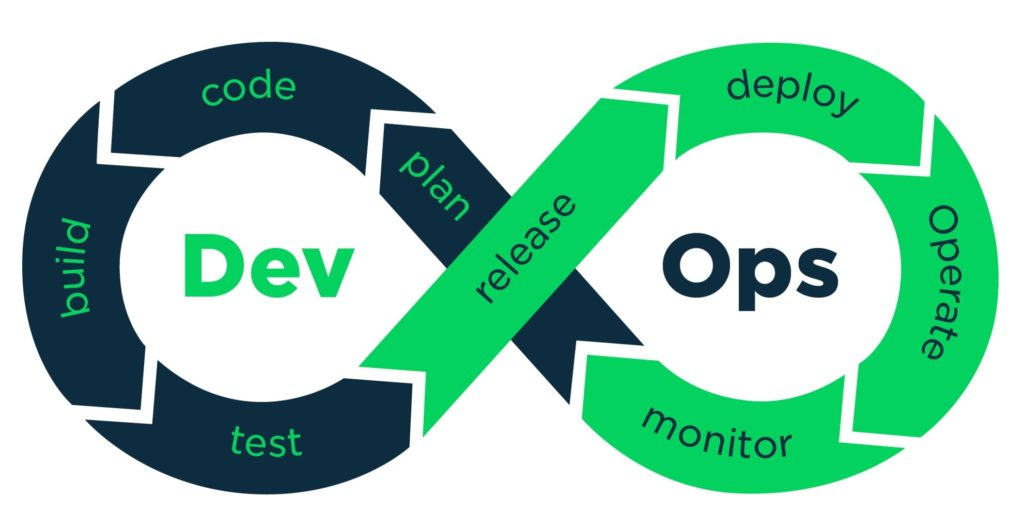
\includegraphics[width=0.6\textwidth]{images/devops_zyklus}
    \caption[DevOps Zyklus]{DevOps Zyklus \footnotemark}
    \label{fig:devops_zyklus}
\end{figure}
\footnotetext{Bildquelle: https://www.mt-ag.com/blog/know-how/devops/mit-jenkins-in-richtung-devops/}

DevOps beschreibt also keine Rolle, Team oder Abteilung und kann somit nicht eingestellt oder gekauft werden.
\footnote{König/Kugel, vgl.~\cite{Konig2019}~[S.292]}
Es geht dabei um mehr als nur um Automatisierung und Infrastructure as Code.
\footnote{Lichtenberger, vgl.~\cite{Lichtenberger2017}~[S.244]}

Die Auflösung von Silos soll die Entwicklung von komplexen Produkten beschleunigen und sicherer machen.
In der Literatur wird hierzu das \textbf{CAMS Model} genannt:
\footnote{Kasteleiner/Schwartz, vgl.~\cite{Kasteleiner2019}~[S.211-214]}
\footnote{Mazzara, vgl.~\cite{Mazzara2019}~[S.104]}

\begin{itemize}
    \item \textbf{Culture:}
    Kultureller Wandel ist einer der wichtigsten Aspekte von DevOps.
    Dabei sind die Nutzung von Scrum, Auflösung von Silos und der Wille in die umfangreiche Investition in die Weiterentwicklung maßgebend.

    \item \textbf{Automation:}
    Automatisierung und Vermeidung von manuellen Übergabeprozessen ist notwendig, um den Informationsfluss zu beschleunigen und Fehler zu vermeiden.

    \item \textbf{Measurement:}
    Kontinuierliche Verbesserung stellt eine der Kernkomponenten dar.
    Durch Metriken können Verbesserungen festgestellt und Verbesserungspotenziale identifiziert werden.


    \item \textbf{Sharing:}
    Transparenz und Wissenstransfer sind notwendig, um ein gemeinsames Wissen zu schaffen.
\end{itemize}

%Die Literatur benennt noch weitere Kombinationen dieses Kunstworts.
%Das wird häufig auch als StarOps bezeichnet zusätzliche Bezeichnungen sind hier:
%ArchOps, BizDevOps, SecDevOps, NoOps, AgileOps.
%\footnote{König/Kugel, vgl.~\cite{Konig2019}~[S.292]}


%    [RESTE]
%    X Testing hypotheses, organizational success is a common goal, reduce fricton, small independent teams deliver sw with self service tools, quick, safe and reliable, maximize developer productivity `(Kim et al)`
%    X Auflösung von Silos `(Schwarz/Kasteleiner)`
%    - DevOps is a recent approach that intends to improve the collaboration between development and IT operations teams, in order to establish a continuous and efficient deployment process. `(Siebra, 427)`
%    - a  set  of  practices  intended  to  reduce  the  time  between  committing  a  change  to  a  system  and  the  change  being  placed  into normal production, while ensur-ing  high  quality. `(Ozkaya, 3)`
%    - DevOps ist mehr => Lernzyklus beschleunigen, Zusammenarbeit der Fachabteilungen `(Schwarz/Kasteleiner)`
%    - DevOps as a concept for integrating the tasks, knowledge, and skills pertaining to the planning, building, and running of activities in a single cross- functional team that is responsible for the combined development and operational tasks of one or more software service products `(Wiedemann, 157)`
%    X Voraussetzung für DevOps: Automatisierte Prozesse in hoher Qualität und minimale Übergaben `(Schwarz/Kasteleiner)`
%    X Individual Software als Hauptprodukt eines Unternehmens `(Schwarz/Kasteleiner)`
%    X DevOps entails a series of socio-technical and organizational practices and tools that address and tackle these distances one by one until a frictionless, fluent, and resilient organization is distilled. (use of the same knowledge-base) `(Artac, Nitto, P. 497)`
%    - Standardsoftware einmal gekauft, Verbesserungen automatisch `(Schwarz/Kasteleiner, 1ff)`
%    X DevOps ist keine Rolle, Team, Abteilung, Toolchain Prüfsiegel oder Regulierung die eingestellt, gekauft oder erfüllt werden kann. `(König/Kugel, P. 292)`
%    X Software development processes  that  replace  communica-tion  with  over-the-wall  tasks  conse-quently  fail

\subsubsection{Geschichte}\label{devops_geschichte}

Das Wasserfallmodell stellt den klassischen Ansatz bei der Entwicklung von Software dar.
Dieser besteht aus den dargestellten aufeinanderfolgenden Stufen:

\begin{figure}[htb]
    \centering
    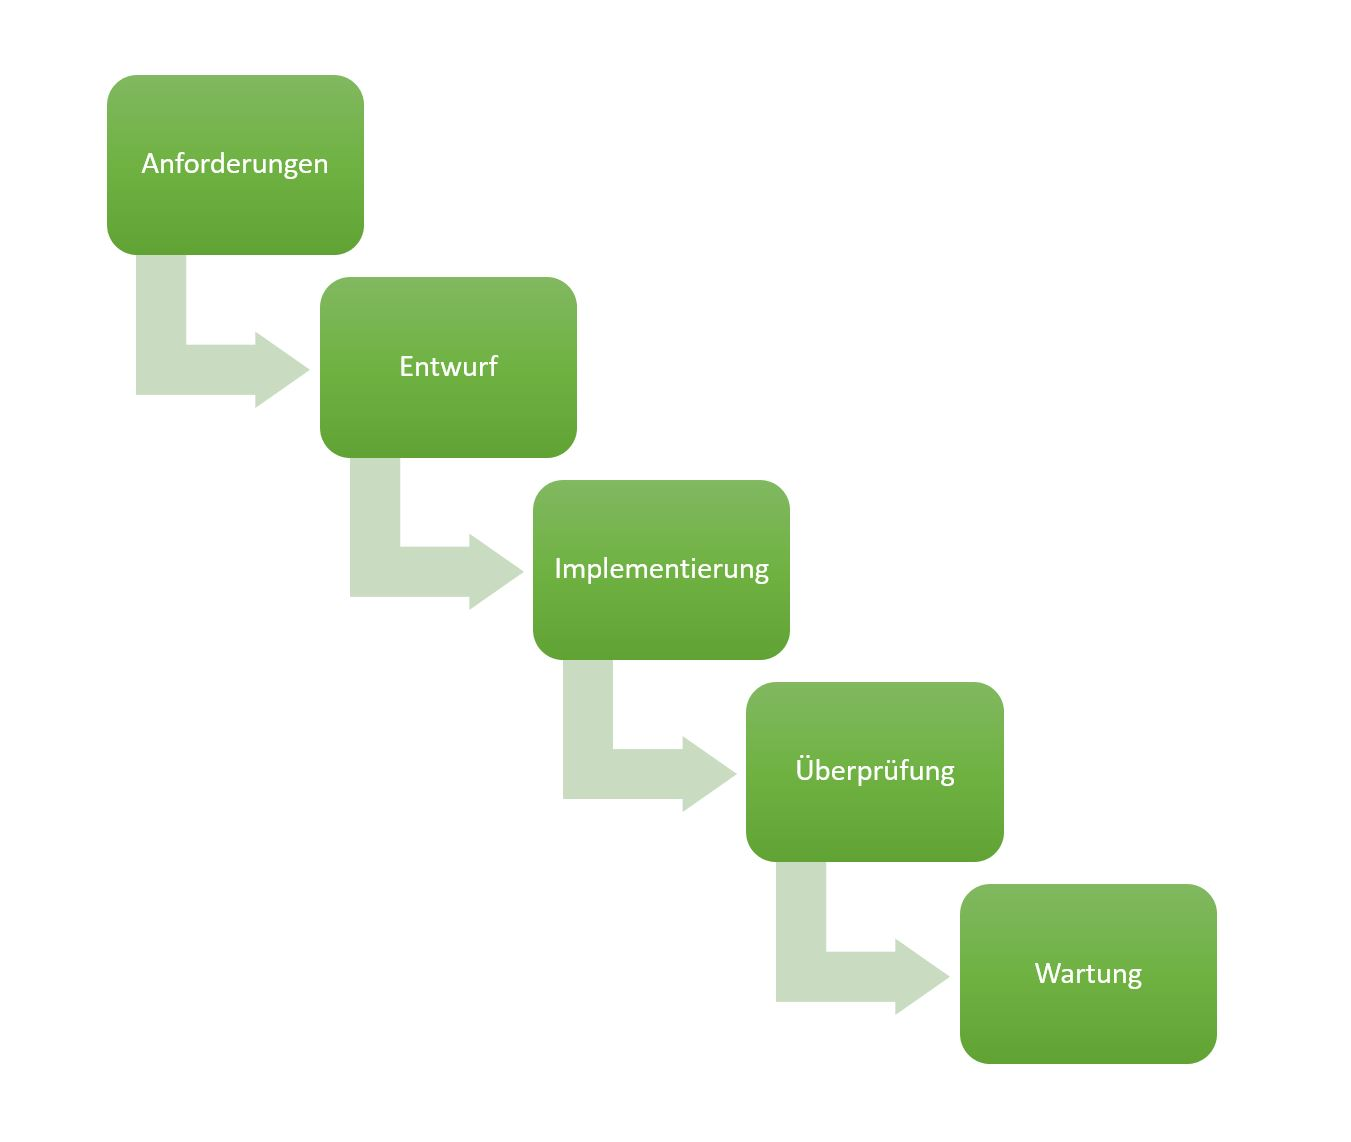
\includegraphics[width=0.8\textwidth]{images/wasserfall.jpg}
    \caption[Wasserfallmodell]{Wasserfallmodell}
    \label{fig:Wasserfallmodell}
\end{figure}

\begin{itemize}
    \item \textbf{Anforderungen:} Basierend auf einem Lasten- oder Pflichtenheft.
    \item \textbf{Entwurf:} Spezifikation und Dokumentation der Software.
    \item \textbf{Implementierung:} Entwicklung der Software auf Basis des Entwurfs.
    \item \textbf{Überprüfung:} Prüfung der Korrektheit mithilfe von Tests.
    \item \textbf{Wartung:} Pflege der Software mittels Updates bei Fehlern oder Sicherheitsproblemen.
\end{itemize}

Dieser Ansatz vernachlässigt, dass gerade in Unternehmen deren Hauptprodukt Software ist,
diese nie \textsl{fertig} ist und auch nach Fertigstellung der ersten Version weiterentwickelt werden muss.
\footnote{Kasteleiner/Schwartz, vgl.~\cite{Kasteleiner2019}~[S.211-214]}

Darüber hinaus hat das Modell die Einschränkung, dass die Phasen in der Realität nicht immer abgeschlossen werden können,
da die Anforderungen essenzieller Bestandteil für eine funktionierende Anwendung des Models sind.
Die Anforderungen müssen zuvor kommuniziert und festgelegt werden.
\footnote{Armenise, vgl.~\cite{Armenise2015}~[S.24]} \\

Im Buch: \textsl{The mythical man-month} von 1975, schreibt Fred Brooks: \footnote{Ozkaya, vgl.~\cite{Ozkaya2019}~[S.3]}

\begin{quotation}
    \textsl{Die meisten großen vergangenen Fortschritte in der Software Produktivität wurden durch das Entfernen von künstlichen Barrieren erreicht.}
\end{quotation}

Das \textsl{agile Manifest} wurde 2001 verfasst und basiert auf häufiger Auslieferung, leichtgewichtigen Prozessen und selbstmotivierten Teams statt wasserfallartiger Entwicklung.
\footnote{Kim et al., vgl.~\cite{Kim2018}~[S.4-5]}
Der Trend zur Beseitigung von Barrieren entstand als Unternehmen wie Netflix, Etsy und Spotify ihre Entwicklungspraktiken in Richtung DevOps und Lean implementierten.
\footnote{Lichtenberger, vgl.~\cite{Lichtenberger2017}~[S.245]}
Die sogenannten Lean Prinzipien haben sich in der Herstellung von physischen Gütern etabliert.
So wurden in den 80er Jahren weniger als 75\% der Bestellungen pünktlich ausgeliefert,
im Jahre 2005 ist dieser Wert sogar auf über 95\% gestiegen. \footnote{Kim et al., vgl.~\cite{Kim2018}~[S.3-5]}

Einer der Vorreiter in diesem Bereich war der Autohersteller Toyota.
Lean begann bei Toyota im Produktionsprozess (TPS).
Es handelt sich dabei um die Optimierung auf Material- und Informationsfluss statt Zerlegung in viele isolierte Arbeitsschritte.
\footnote{Samulat, vgl.~\cite{Samulat2017}~[S.206]}

Fokussiert wurde der Blick auf die Zeit (schneller Durchlauf des Materials) und die Qualität (beim ersten Mal richtig).
\footnote{Samulat, vgl.~\cite{Samulat2017}~[S.206]}

Als im Jahre 2009 die erste Konferenz zum Thema DevOps in Gent (Belgien) gehalten wurde,
war das Thema nicht ganz neu und wurde von Startups bereits vorgelebt. \footnote{Wiedemann, vgl.~\cite{Wiedemann2019}~[S.158]}
Die Konferenz bestand aus nur 60 Teilnehmer und galt als Start der DevOps-Bewegung,
die unter anderem von den Autoren des \textsl{DevOps Handbooks} wie z.B. Patrick Debois geprägt wurde.
\footnote{König/Kugel, vgl.~\cite{Konig2019}~[S.291]}

Ziel dieser Bewegung ist es, den Graben zwischen Entwicklung und Betrieb zum Wohle der Wertschöpfungskette zu schließen.
Das wird in der DevOps Bewegung auch als \textsl{Flow} bezeichnet. \footnote{Lichtenberger, vgl.~\cite{Lichtenberger2017}~[S.246]}
Dazu werden die sogenannten \textsl{Walls of Confusion}, also den Interessenskonflikten zwischen Entwicklung und Betrieb minimiert bzw. entfernt. \footnote{König/Kugel, vgl.~\cite{Konig2019}~[S.291]} \\

Moderne technische Projekte benötigen mehrere Perspektiven und Expertise. \footnote{Kim et al., vgl.~\cite{Kim2018}}
Die IT-Industrie stellt Prozesse immer noch infrage. \footnote{Samulat, vgl.~\cite{Samulat2017}~[S.206]},
Je weniger Zeremonien innerhalb eines Entwicklungsprozesses existieren, umso höher ist die Erfolgswahrscheinlichkeit. \footnote{Ozkaya, vgl.~\cite{Ozkaya2019}~[S.4]}
Diesen Umstand hat die DevOps-Bewegung erkannt, will dabei jedoch keine \textsl{One-Size-Fits-All}-Lösung sein. \footnote{König/Kugel, vgl.~\cite{Konig2019}~[S.291]}

%    [RESTE]
%    - experiencing increasing frustra- tion with delays and problems releas- ing software to production, while the operations team felt overloaded and constrained. `(Callanan, 53)`
%    - Gründe für DevOps: Digitalisierung, IT Abteilungen im Unternehmen gespalten `(Lichtenberger, 246)`

\subsubsection{DevOps und Agile Methoden}\label{devops_und_agile}

Die Prinzipien des agilen Manifests decken sich mit den Prinzipien von DevOps.
\footnote{Samulat, vgl.~\cite{Samulat2017}~[S.210]}
\footnote{Kim et al, vgl.~\cite{Kim2018}~[S.4 - S.5]} \\

Durch Scrum oder Kanban Boards wird die Arbeit sichtbar und transparent. \footnote{König/Kugel, vgl.~\cite{Konig2019}~[S.296]}
Darüber hinaus behandeln agile Methoden die Softwareentwicklung aus Sicht des Kunden und der Schaffung von Werten für diesen. \footnote{Mazzara, vgl.~\cite{Mazzara2019}~[S.100]}
Die Flexibilität von agilen Methoden kann durch die Erzeugung von sogenannten Minimum Viable Products (MVP) und kleinen Iterationen mit dem Wasserfallmodell nicht erreicht werden. \footnote{König/Kugel, vgl.~\cite{Konig2019}~[S.290]}

Mit agilen Methoden und DevOps lässt sich eine Produktentwicklung erreichen, die schnell und flexibel auf geänderte Anforderungen reagieren kann.
\footnote{Lichtenberger, vgl.~\cite{Lichtenberger2017}~[S.245]}
\footnote{Söllner, vgl.~\cite{Sollner2019}~[S.321]} \\

Durch den Einsatz von DevOps und agilen Methoden lässt sich mit den gleichen Ressourcen mehr erreichen und man kann unter Umständen schneller agieren als seine Mitbewerber.
Der Fokus liegt hier auf den Kunden.
Ebenso ist es hilfreich, um Verschwendung von Ressourcen zu vermeiden.
Ideen können schnell erprobt werden und es kommt seltener zur Entwicklung von nicht benötigten Features.
\footnote{Samulat, vgl.~\cite{Samulat2017}~[S.208 - S.210]}

%    [RESTE]
%    - SW Entwicklung erfordert neues Denken (Lean): `(Samulat, P. 208/210)`:
%    - Digitalisierung stellt Business und IT Strukturen in Frage: Änderungen für jeden Kulturwandel, manchmal auch Revolution
%    - Vermeidung von Verschwendung, Unregelmäßigkeit und übermäßiger Belastung
%    - T Shaped Mitarbeiter
%    - Produkt bzw. Kundenfokus
%    - Strategie kann nicht umgesetzt werden solange noch mit Taktik gekämpft wird.
%    - Commodity IT: Dienstleister stellen IT Leistungen die zu dem Preis von der internen IT nicht mehr zu erreichen sind, Grenze zwischen Kernkompetenz und Unterstützungsfunktion verschiebt sich `(Samulat, P. 209)`
%    - Lean hilft so schnell wie möglich Produkte zu erzeugen, dadurch kann mit den gleichen Ressourcen mehr erreicht wertden und man kann schneller sein als Mitbewerber.
%    - Kultur ist die langsamste und komplexeste Stellschraube im Unternehmen, "Change in Mind" erforderlich
\newpage
\subsubsection{Wege zu DevOps}\label{devops_wege}

In der Literatur werden drei Wege bzw. Eckpfeiler für die Einführung erwähnt.
In jedem Fall ist die Verwendung von DevOps eine Investition in Mitarbeiter, Prozesse und Technologien.
\footnote{Kasteleiner/Schwartz, vgl.~\cite{Kasteleiner2019}~[S.211-214]}

Dabei gilt, dass eine solche Einführung niemals als abgeschlossen angesehen werden kann.
\footnote{König/Kugel, vgl.~\cite{Konig2019}~[S.292 - S.293]}
\footnote{Kim et al, vgl.~\cite{Kim2018}}

Diese drei grundsätzlichen Wege von DevOps werden in der Literatur genannt:

\begin{itemize}
    \item \textbf{Flow:}
    Praktiken, um die Zusammenarbeit zwischen den Abteilungen zu verbessern.
    Alles dient dem Ziel die Wertschöpfung für das Unternehmen zu optimieren.

    \item \textbf{Feedback:}
    Um die nächsten Schritte besser bestimmen zu können, sollen die Erfahrungen und Metriken aus dem Betrieb in die Entwicklung zurückfließen.

    \item \textbf{Continuous Learning and Experimentation:}
    Die gesamte Organisation soll die Wertschöpfungskette zum Kunden verstehen und aus den bisherigen Metriken lernen.
\end{itemize}

Um das Experimentieren zu fördern, sollte eine Kultur geschaffen werden in der Fehler toleriert werden.
Dabei sollten Review Prozesse jedoch sicherstellen, dass es durch Fehler zu keinen größeren Ausfällen kommen kann.

Die Einführung von agilen Methoden wie z.B. Scrum einer der ersten Schritte sein, um DevOps zu ermöglichen.
Dies macht Prozesse transparent und erlaubt die Priorisierung von Aufgaben.
\footnote{Kim et al, vgl.~\cite{Kim2018}~[S.16 - S.17]} \\

Der jährlich erscheinende \textsl{State of DevOps Report} von Puppet hat ermittelt, dass die Einführung von DevOps insbesondere für die Produktentwicklung und nicht so sehr für konkrete Projektarbeit geeignet ist.
Das liegt vorallem daran, dass bei Projekten die Anforderungen klarer definiert sind als bei der Entwicklung von Produkten.
\footnote{Wiedemann, vgl.~\cite{Wiedemann2019}~[S.164]}
\footnote{Puppet State of DevOps Report 2020, vgl.~\cite{PUPPET}}

\newpage
\paragraph{Maßnahmen}\label{devops_massnahmen}

Zur Anwendung von DevOps benötigt ein Unternehmen einige technische und organisatorische Maßnahmen.
In der Literatur finden sich hierzu folgende Gemeinsamkeiten:
\footnote{Buchan et. al, vgl.~\cite{Senapathi2018}~[S.2]}
\footnote{Callanan, vgl.~\cite{Callanan2016}~[S.56 - S.57]}
\footnote{Schwarz/Kasteleiner, vgl.~\cite{Kasteleiner2019}~[S.211 - S.214]}

\begin{itemize}
    \item \textbf{Automatisierung:}
    Aufgaben die mehr als zweimal manuell gemacht wurden, sollte automatisiert werden. \footnote{Ozkaya, vgl.~\cite{Ozkaya2019}~[S.3]}

    \item \textbf{Kollaboration und Embedded OPS:}
    Mitarbeiter aus der Betriebsabteilung sollten in die Entwicklungsteams integriert werden.  \footnote{König/Kugel, vgl.~\cite{Konig2019}~[S.294]}

    \item \textbf{Kontinuierliche Entwicklung:}
    Prozesse und Mitarbeiter sollten kontinuierlich weiterentwickelt und optimiert werden.

    \item \textbf{Fokus auf den Kunden:}
    Prozesse und Tätigkeiten sollten stets auf deren Kundennutzen überprüft werden.
    Prozesse, die keinen Wert für den Kunden erzeugen, sollten entfernt werden. \footnote{Ozkaya, vgl.~\cite{Ozkaya2019}~[S.5]} \footnote{Samulat, vgl.~\cite{Samulat2017}~[S.214]}

    \item \textbf{Selbstorganisierte Teams:}
    Kleine selbstorganisierte Teams mit End-to-End-Verantwortung (\textsl{You build it, you run it}). \footnote{Lichtenberger, vgl.~\cite{Lichtenberger2017}~[S.245]}

    \item \textbf{Continuous integration und Testing:}
    Einbindung automatischer Prozesse für Build, Test und Deployment ermöglichen.

    \item \textbf{Continuous Release und Deployment:}
    Durch Automatisierung sollte es einen Weg von Software in die Produktivsysteme geben. \footnote{Buchan et. al, vgl.~\cite{Senapathi2018}~[S.3]}

    \item \textbf{Continuous Monitoring:}
    Infrastruktur und User Verhalten sollten überwacht werden.
    Die Metriken können dann in der Entwicklung berücksichtigt werden.

    \item \textbf{IaC:}
    Infrastruktur sollte replizierbar sein.
    Durch den Einsatz von IaC lässt sich das erreichen.

    \item \textbf{Wiederherstellung:}
    Bei Problemen sollte es einfach möglich sein vorherige Versionen wiederherszustellen, um Ausfälle kurz zu halten.

    \item \textbf{Self Service:}
    Entwickler können selbst die Infrastruktur erstellen, welche sie für ihre Entwicklung benötigen. \footnote{König/Kugel, vgl.~\cite{Konig2019}~[S.293 - S.294]}
\end{itemize}

\paragraph{Migration zu DevOps}

Besonders in Unternehmen, die bereits ohne DevOps Software entwickeln und diese betreiben, lässt sich nicht von jetzt auf gleich eine DevOps Strategie einführen.
Hierzu finden sich in der Literatur folgende mögliche Vorgehensweisen zur nachträglichen Einführung:

Durch Spin-Offs oder Tochterunternehmen können neue Projekte auf der sogenannten \textsl{grünen Wiese} gestartet werden.
Diese werden dann nach und nach in das Unternehmen zurückgeführt. \footnote{Wiedemann, vgl.~\cite{Wiedemann2019}~[S.164]}

Bei einer Umstellung ist es für die Organisation wichtig, einen frühen Erfolg zu erzielen.
Hierzu empfiehlt es sich, kleine inkrementelle Schritte vorzunehmen. \footnote{Kim et al, vgl.~\cite{Kim2018}~[S.58 - S.59]}
% Dabei ist es hilfreich Unterstützung von Nachahmern des Ansatzes zu finden, diese Innovatoren im Unternehmen kann man dan dazu nutzen eine kritische Masse zu erreichen.
% Das Unternehmen Wotif aus Australien hat nach ihrer DevOps Migration ihre Zyklen für das Ausrollen neuer Software von zwei Wochen auf einen Tag verkürzt. \footnote{Callanan, vgl.~\cite{Callanan2016}~[S.56 - S.57]}

\paragraph{DevOps Reifegrade}\label{devops_reifegraden}

Das DevOps Evolution Model wird im jährlichen State Of DevOps Report von Puppet Labs veröffentlicht \footnote{Puppet State of DevOps Report 2020, vgl.~\cite{PUPPET}~[S.10]}
Dort wird der Reifegrad einer DevOps Einführung mittels mehrerer Stufen bewertet:

\begin{figure}[htb]
    \centering
    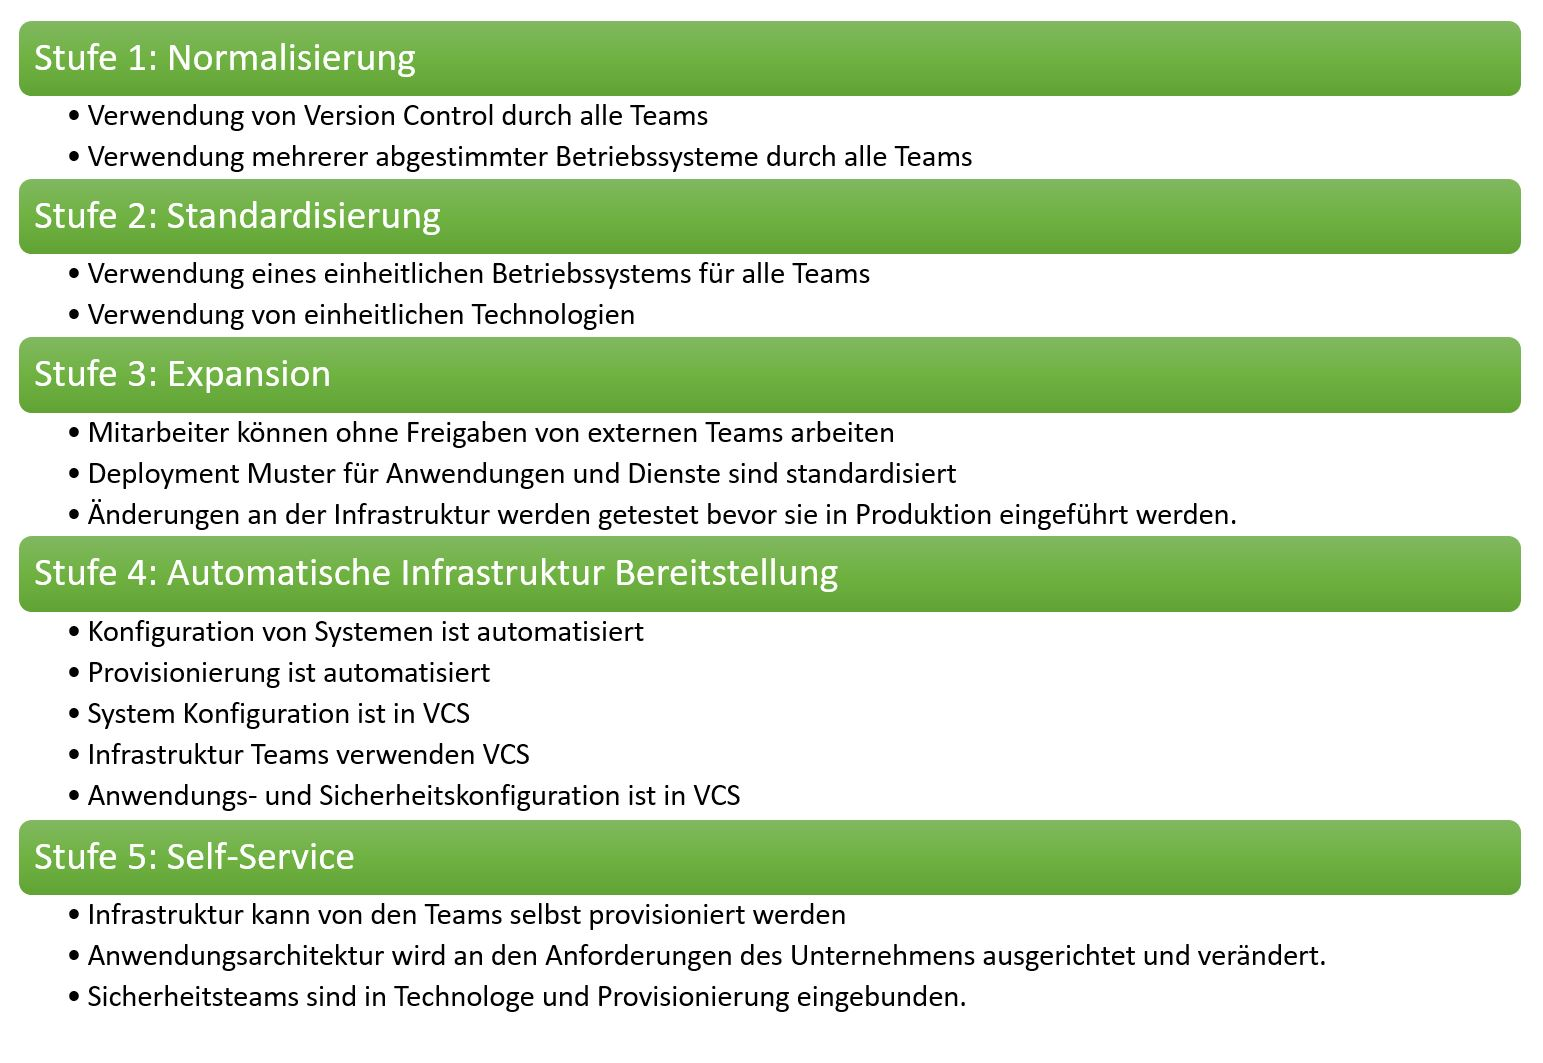
\includegraphics[width=1.0\textwidth]{images/devops_reifegrad.jpg}
    \caption[DevOps Reifegrade]{DevOps Reifegrade}
    \label{fig:DevOps Reifegrade}
\end{figure}

Anhand dieses Models kann ein Unternehmen den eigenen Fortschritt somit überwachen und die weiteren Schritte planen.

%    [RESTE]
%    - A  common  goal  of  all  processes  is  to   eliminate   nonessential   activities   that  consume  resources  away  from  development  and  delivery  of  function-ality  that  provides  quality  to  its  us-ers `(Ozkaya, 5)`
%    - Prozesse auf Kundennutzen prüfen, Kundenwünsche erkennen, nicht werterzeugende Prozesse eliminieren, Trasnsparenz und Qualitätsicherung, Kontiniuierliche Verbesserung `(Samulat, P. 214)`
%    - IT der zwei Geschwindigkeiten (Porter Kurver IT), Economy of Scope vs Scale `(Samulat, P. 207)`
%    - Economy of Scope: Pro Kunde individuell, Einzelfertigung, Individuelle Prozesse
%    - Economy of Scale: Preis/Mengen Strategie, Massenfertigung, Standardprozesse
%    - Mike Gualtieri (2011): "NoOps means application developer will never have to speak to an operations professional again" `(König/Kugel, P. 290)`
%    - Higher levels of DevOps means more self-service offerings for developers, 63% of participants have at least one `(https://puppet.com/resources/report/2020-state-of-devops-report/)`


\subsubsection{Vorteile}\label{devops_vorteile}

Durch die Einführung von DevOps erhalten Unternehmen einerseits Wettbewerbsvorteile und andererseits aber auch Verbesserungen für Kunden und Mitarbeiter.
\footnote{König/Kugel, vgl.~\cite{Konig2019}~[S.293]}
\footnote{Buchan et. al, vgl.~\cite{Senapathi2018}~[S.7-8]}

\begin{itemize}
    \item \textbf{Time-To-Market:}
    Diese Zeit kann verkürzt werden.
    Die Unternehmen erhalten Wettbewerbsvorteile, da sie schneller auf Mitbewerber oder neue Kundenanforderungen reagieren können. \footnote{Lichtenberger, vgl.~\cite{Lichtenberger2017}~[S.245]}
    Produktideen können zügiger ausprobiert werden, um so bestimmte Hypothesen schneller prüfen zu können.

    \item \textbf{Erhöhte Stabilität:}
    Geringere Fehleranfälligkeit durch kleinere Releases und erhöhte Automatisierung. \footnote{Lichtenberger, vgl.~\cite{Lichtenberger2017}~[S.246]}
    Fehler können kostengünstiger behoben werden, da sie zeitnah entdeckt und Systeme schneller aktualisiert werden können.

    \item \textbf{Konflikte:}
    Überwindung von Konflikten zwischen den Abteilungen durch die Beseitigung der \textsl{Wall of Confusion}.
    Hand offs zwischen den Abteilungen werden minimiert oder sogar entfernt.
    Die Teams sind kleiner und selbstorganisiert, dadurch können sie selbstständiger arbeiten. \footnote{Lichtenberger, vgl.~\cite{Lichtenberger2017}~[S.246]}
    Formale Übergaben entfallen durch Tests und Automatisierung \footnote{Kasteleiner/Schwartz, vgl.~\cite{Kasteleiner2019}~[S.211-214}

    \item \textbf{Change Management:}
    Durch den Einsatz von Infrastructure as Code sind Änderungen besser nachvollziehbar und dokumentiert.
    Die Verwendung von Ticketsystemen, Scrum und IaC verbessert das Change Management. \footnote{Puppet State of DevOps Report 2020, vgl.~\cite{PUPPET}~[S.24 - S.26]}

    \item \textbf{Arbeitsbedingungen:}
    Mitarbeiter sind motivierter, da die Arbeitsbedingungen kontinuierlich optimiert werden.
    Entwickler können innovativer sein und selbstständig Ideen ausprobieren, die dem Kunden schneller einen Mehrwert bieten.
\end{itemize}


Laut Lichtenberger gilt oft der Grundsatz:

\begin{quotation}
    \textsl{Nicht der große Fisch frisst den kleinen, sondern der schnelle den langsamen.}
    \footnote{Lichtenberger, vgl.~\cite{Lichtenberger2017}~[S.248]}
\end{quotation}

Dieser Grundsatz zeigt, warum auch große Unternehmen an einer Beschleunigung ihrer Prozesse bei der Entwicklung und dem Betrieb von Software interessiert sein sollten. \\

Die australische Hotelbuchungswebsite Wotif hat z.B. durch die Einführung von DevOps die Releasezyklen von zwei Wochen auf einen Tag verkürzt und den Prozentsatz von Problemen,
die den Kunden betreffen, von 15\% auf 7\% gesenkt.
\footnote{Callanan, vgl.~\cite{Callanan2016}~[S.57]}


%    [RESTE]
%    - SlipWay: Team Moral erhöht `(Callanan, 59)`
%    - Übergeordnete Ziele von DevOps `(König/Kugel, P. 293)`
%    - Überwindung des chronischen IT-Konflikts - Wall of Confusion einreißen
%    - Häufige SW Releases erleichtern und optimieren
%    - Kontiniuierliche Verbesserung der Arbeitsbedingungen
%    - Erhöhung von Stabilität und Sicherheit
%    - Weg von der Idee bis zum Kunden optimieren
%    - Benefits from study of `(Buchan, 7-8)`:
%    - Teams happier and more engaged
%    - More frequent releases, smaller releases
%    - DevOps umgesetzt: Doppelt profitieren (Kundenanforderungen/ Motivation Mitarbeiter) `(Schwarz/Kasteleiner)`
%    - Produktideen sind Hypothesen `(Schwarz/Kasteleiner)`
%    - “It just means you are not relying on other teams to do the infrastructure. You have control over it – choice of tool to use for example. To get the feel of small startups in a big organisation” [Developer. `(Buchan, 6)`
%    - Product teams felt more valued in the new DevOps way of functioning. The embedded ops did not feel that they were just sitting in the dark maintaining servers and databases, but could see the value and impact of their work on real clients `(Buchan, 7)`
% \subsubsection{Herausforderungen}\label{devops_herausforderungen}

Bei der Einführung von DevOps müssen sowohl technische als auch organisatorische Herausforderungen bewältigt werden.
Häufig wird Software jedoch unter Zeitdruck entwickelt und für die Verbesserung von Organisatorischen sowie technischen Problemen wird keine Zeit vorgesehen.
\footnote{Lichtenberger, vgl.~\cite{Lichtenberger2017}~[S.244]} \\

Bei zahlreichen Musterunternehmen für die DevOps Bewegung wie Netflix und Spotify wurden auf der \textsl{Grünen Wiese} gestartet und diese konnten die Themen von Anfang an angehen.
\footnote{Lichtenberger, vgl.~\cite{Lichtenberger2017}~[S.247 - S2.248]}

\paragraph{Organisatorisch}

Wenn DevOps Transformationen gestartet werden, ohne dass die Stakeholder und die Geschäftsleitung eine Notwendigkeit dafür sieht,
so scheitern ca. 50\% aller Transformationen bereits zu Beginn. \footnote{Lichtenberger, vgl.~\cite{Lichtenberger2017}~[S.246]} % `(Kotter 2012)`
Es ist notwendig einen sogenannten \textsl{Sense of Urgency} bei der Geschäftsführung und den Entscheidern zu wecken und diese
davon zu überzeugen das diese Transformation notwendig ist. \footnote{Wiedemann, vgl.~\cite{Wiedemann2019}~[S.165]}
Es darf nicht vernachlässigt werden, dass eine solche Veränderung viele Ressourcen kostet und der Wert nicht sofort ersichtlich ist. \\

Wenn das Unternehmen trotz fehlender DevOps Strategie erfolgreich ist, kann es schwierig sein diese Veränderungen zu erklären.
Unter Zeitdruck, können Konflikte alleine dadurch entstehen, dass bestimmte Aufgaben zwecks
Organisationalem Lernen auf Personen verteilt werden, welche auf den ersten Blick nicht die erfahrensten für diese Aufgaben sind.\footnote{Samulat, vgl.~\cite{Samulat2017}~[S.206]}
Diese zunächst unvermeidliche Verlangsamung muss vom Management unterstützt werden.
Eine der Grundannahmen von DevOps ist auch, dass Fehler gemacht werden dürfen, wenn auch die Konsequenzen dieser Fehler minimiert werden müssen.
Eine Kultur in der Fehler gemacht werden dürfen, hängt ganz entscheidend von der Reaktion des Managements auf diese Fehler ab. \footnote{Kim et al, vgl.~\cite{Kim2018}~[S.38]} \\

Darüber hinaus ist eine DevOps Transformation ebenfalls eine große Veränderung der bisherigen Arbeitsweisen. \footnote{Wiedemann, vgl.~\cite{Wiedemann2019}~[S.163]}
Die Angst vor Veränderung, die Kosten für Schulungen bzw. Weiterbildungen und die Verlangsamung von Prozessen zu Beginn ihrer Umstellung
ist ebenfalls zu berücksichtigen. \footnote{Kasteleiner/Schwartz, vgl.~\cite{Kasteleiner2019}~[S.211-214]}

\paragraph{Technisch}

Der technische Aspekt einer DevOps Strategie erfordert häufig eine ganze Reihe von neuen Technologien. \footnote{Puppet State of DevOps Report 2020, vgl.~\cite{PUPPET}~[S.3]}
Dafür müssen neue Technologien erlernt und eingeführt werden, Systeme umgestellt werden und vor allem Automatisierung eingeführt werden. \footnote{Samulat, vgl.~\cite{Samulat2017}~[S.205]}
Gerade die Automatisierung kann viele Unternehmen überfordern. \footnote{Samulat, vgl.~\cite{Samulat2017}~[S.211]}

Um höhere DevOps Reifegrade zu erreichen, muss eine Self Service Plattform geschaffen werden, diese lässt sich ohne
den Einsatz von SaaS Lösungen von Cloud Anbietern nicht umsetzen. \footnote{Kasteleiner/Schwartz, vgl.~\cite{Kasteleiner2019}~[S.211-214]}

Das DevOps Mantra welches von Netflix praktiziert wird lautet:

\begin{quotation}
    \textsl{You build it, you run it.}
    \footnote{König/Kugel, vgl.~\cite{Konig2019}~[S.296 - S.297]}
\end{quotation}

Um Systeme zu betreiben, müssen die Entwickler Wissen aus dem Bereich des Betriebs haben und umgekehrt.
Selbst wenn die Teams durchmischt sind mit Entwicklern und Administratoren, so kann es doch einige Zeit dauern
bis durch Knowledge Sharing das Wissen ausreichend verteilt wurde. \footnote{Puppet State of DevOps Report 2020, vgl.~\cite{PUPPET}~[S.3]}


%    \paragraph{Zusammenfassung}
%
%    - Funktionale Trennung aus Dev und Ops auflösen, interdisziplinäre Teams mit gemeinsamen Zielen und Anreizen. \footnote{Lichtenberger, vgl.~\cite{Lichtenberger2017}~[S.244]}
%    - "Culture eats Strategy for Breakfast" \footnote{Lichtenberger, vgl.~\cite{Lichtenberger2017}~[S.246]}
%    - No process definition will magi-cally deliver results without a committed, disciplined team, and organization behind it  \footnote{Ozkaya, vgl.~\cite{Ozkaya2019}~[S.4]}
%    [RESTE]
%    - "Unicorns" hatten einfache Vorraussetzungen, das die Projekte auf der Grünen Wiese gestartet sind. (IaC, Pipelines konnten von Anfang an integriert werden) `(Lichtenberger, 247-248)`
%    - DevOps ist nie das Ziel, sondern Mittel zum Zweck `(Lichtenberger, 246)`
%    - Organisation soll Lernen `(Schwarz/Kasteleiner)`
%    - Lack of Time, Standardization, Technical skill within the team `(https://puppet.com/resources/report/2020-state-of-devops-report/, )`
%    - Challenges in Adopting DevOps During `(Buhan, 8-9)`
%    - Having staff with the right technical skills
%    - Resistance to Change and Uncertainty
%    - Changing the Technology Stack and Tools
%    - Uncertainty in Responsibilities
%    - Dev will Veränderung, Ops will Stabilität: SW aus Zeitdruck häufig nicht unter Berücksichtung von Ops Problemen entwickelt \footnote{König/Kugel, vgl.~\cite{Konig2019}~[S.291]}
%    - Kosten/Risiken: Angst vor Veränderung, Schulungen und Weiterbildungen, Prozesse können während der Umstellung mehr Zeit benötigen
%    - Sharing knowledge is a key factor in the DevOps movement [BC13]. These knowledge-sharing activities are helpful because the teams learn from e
%    - Metriken sammeln um Ideen zu verifizieren \footnote{Kasteleiner/Schwartz, vgl.~\cite{Kasteleiner2019}~[S.211-214]}

% CI/CD
\newpage
\subsection{Continuous Integration, Deployment und Delivery}\label{continouous_whatever}

Die Begriffe Continuous Integration, Deployment und Delivery sind eng miteinander verbunden und werden häufig als Abkürzung CI/CD verwendet.
Eine sogenannte CI/CD Pripeline besteht dabei aus mehreren ineinandergreifenden Komponenten: \footnote{Shweta et. al, vgl.~\cite{Shweta2014}~[S.214]} \\

\begin{figure}[htb]
    \centering
    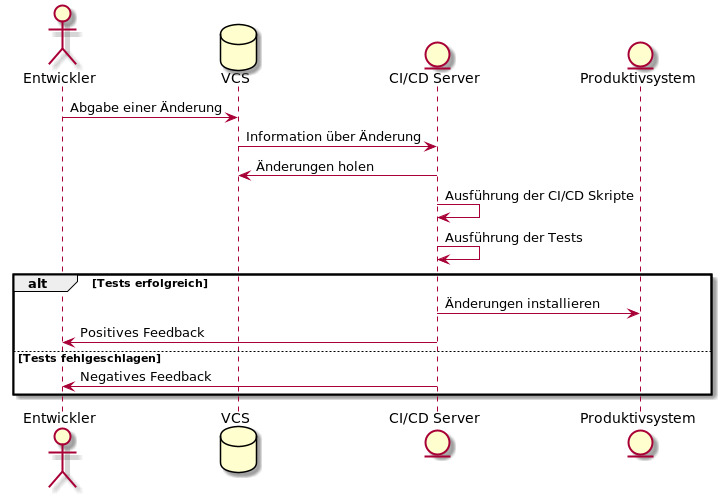
\includegraphics[width=1.0\textwidth]{images/cicd_pipeline.jpg}
    \caption[Vereinfachte CI/CD Pipeline]{Vereinfachte CI/CD Pipeline}
    \label{fig:Vereinfachte CI/CD Pipeline}
\end{figure}


%\begin{itemize}
%    \item \textbf{Entwickler:} Mitarbeiter die Quellcode verändern
%    \item \textbf{VCS:} Versionsverwaltung zur Zusammenarbeit am Code
%    \item \textbf{CI/CD Server:}
%    \item \textbf{CI/CD Skripte/Konfiguration:}
%    \item \textbf{Feedback:}
%    \item \textbf{Produktivsystem:}
%\end{itemize}


%- Versionskontrolle (VCS): Der Quellcode sollte in einem System zentral verwaltet werden.
%- CI Server: Ein System das die Änderungen aller Entwickler automatisch, zusammenführt, testet und je nach Konfiugration sogar ausrollt.
%- CI Skripte/Konfiguration: Einem CI Server muss per Skript oder Konfiguration mitgeteilt werden wie ein Projekt zu kompilieren, testen und zu deployen ist. In der Regel werden diese Skirpte zusammen mit dem Quellcode im VCS gehalten.
%- Feedback Mechanismen: Wenn ein Entwickler einen CI/CD Job started kann es unter Umständen einen Moment dauern bis das Ergebnis feststeht, daher sollte ein CI Server Benachrichtigungen in Form von E-Mails oder Kommentaren in dem entsprechenden VCS haben.

\subsubsection{Versionsverwaltung}\label{vcs}

Ein VCS (auch SCM System genannt) ist eine Software mit der die Änderungen an Dateien nachverfolgt und bei Bedarf wieder zusammengeführt werden können.
Es ermöglicht mehreren Personen Änderungen an dem gleichen Quellcode nachvollziehbar durchführen zu können.
Jeder hat seine eigene Kopie des Quellcodes.
Das zurzeit am meisten verwendete SCM ist Git.
Es wird unter anderem bei Google, Facebook, Microsoft und der Linux Entwicklung verwendet. \footnote{Git Website, vgl.~\cite{GIT_SCM}}
Git ist über die Kommandozeile bedienbar.
Es sind jedoch ebenfalls zahlreiche grafische Tools verfügbar.
Teilweise sind diese auch bereits in Entwicklungsumgebungen (IDE) integriert.

\paragraph{Repository}

Ein Repository ist ein Ordner in dem sich ein \texttt{.git} Ordner befindet.
Hier wird die Historie und alle Branches verwaltet. \footnote{Git Basics, vgl.~\cite{GIT_SCM_BASICS}}
Werden Dateien in diesem auch als \textsl{Working Directory} bezeichneten Ordner verändert, dann lassen sich diese Änderungen mit Git erfassen.
Es wird dabei zwischen \textsl{Unstaged-} und \textsl{Staged}-Änderungen unterschieden.

\paragraph{Remote}

Git ist dezentral.
Ein Repository kann ein oder mehrere Remotes haben.
Dabei handelt es sich um Server auf denen der jeweilige Branch mit einem \textsl{Push} aktualisiert werden kann.
Es muss keine Remotes haben.
So ist es möglich Git auch ohne Internetverbindung zu verwenden.
Der dezentrale Ansatz sorgt dafür, dass jeder Entwickler, auf eine vollständige Kopie des ausgecheckten Codes Zugriff hat.
\footnote{Git Basics - Working with Remotes, vgl.~\cite{GIT_SCM_REMOTES}}

\paragraph{Branch}

Ein Entwicklungszweig, der die versionierten Dateien enthält, wird als \textsl{Branch} bezeichnet.
In der Regel gibt es einen Hauptbranch welcher als \textsl{Master} bezeichnet wird.
Von diesem wird abgezweigt. \footnote{Git Branching - Branches in a Nutshell, vgl.~\cite{GIT_SCM_BRANCHING}}
Jeder Entwickler führt seine Änderungen auf seinem Branch durch und anschließend können diese Änderungen wieder in den Hauptzweig überführt werden.

\paragraph{Commit}

Änderungen die \textsl{Staged} sind können zu einem Commit zusammengefasst werden.
Ein Commit besteht aus den Veränderungen (Diffs) und einer Commit Message vom Entwickler.
Er wird immer auf einem Branch durchgeführt.
Jeder Commit erhält einen Hash-Wert und kann einen Parent-Hash-Wert haben.
Durch diese Hashes kann Git die Änderungshistorie aufbauen und nachvollziehen, wie Änderungen wieder zusammenzuführen sind.

\begin{figure}[htb]
    \centering
    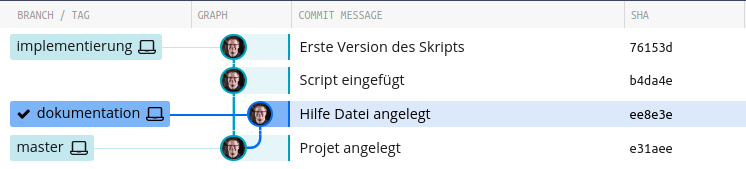
\includegraphics[width=0.8\textwidth]{images/gitkraken_screenshot.png}
    \caption[Commits und Branches in Git]{Commits und Branches in Git}
    \label{fig:Screenshot aus dem Git Client GitKraken}
\end{figure}

\paragraph{Pull/Merge Request}

Um immer einen funktionierenden Stand zu haben wird der Master Branch geschützt, d.h. dass kein direkter Push von Commits auf den Master Branch erfolgen kann.
Damit Code in den Master Branch eingefügt werden kann, werden sogenannte Pull bzw. Merge Request verwendet.
Der Entwickler, der neuen Code auf seinem Branch erstellt hat, erstellt einen Pull Request.
Über die Benutzeroberflächen von Git Kollaborationssoftware (z.B. Gitlab, GitHub, Bitbucket) können so die Änderungen eingesehen und kommentiert werden.
Darüber hinaus kann ein PR/MR dazu verwendet werden auf einem CI Server einen Arbeitsablauf zu starten. \footnote{About pull requests, vgl.~\cite{GITHUB_ABOUT_PR}} \\

%\paragraph{Fork}
%
%- Merge: Führt Änderungen aus einem anderen Branch in den aktuellen Branch ein.
%- Rebase: Hängt die Änderungen auf dem aktuellen Branch an die Änderungen des gewünschten Branches an.
%- Pull/Merge Request:
%- Merge Conflict: Ein Konflikt tritt immer dann auf wenn zwei Entwickler auf unterschiedlichen Branches die gleichen Zeilen bearbeitet haben. Git kann dann nicht mehr unterscheiden welche Änderung genommern werden soll und dieser Konflikt muss manuell aufgelöst werden.
%- Fork: Dieser Begriff kommt vor allem im Zusammenhang mit Open-Source Repositories vor, bei einem Fork erstellt der Entwickler eine Kopie des Repositories in seinem eigenen Account, dort kann er dann Branches anlegen und anschliessend einen Pull Request machen. `(https://docs.github.com/en/free-pro-team@latest/github/getting-started-with-github/fork-a-repo)`

Ein Ansatz aus Scrum und DevOps ist die Annahme, dass der Master Branch immer in einem Zustand ist in dem eine stabile und funktionsfähige Software an den Kunden geliefert werden könnte.
\footnote{Armenise, vgl.~\cite{Armenise2015}~[S.24]}
\subsubsection{Continouous Integration}\label{ci}

Die von Git und anderen VCS Systemen durchgeführte Prüfung auf Konflikte bezieht sich rein auf Konflikte der Datei- und Zeilenebene.
Im Falle von Konflikten muss ein Entwickler entscheiden, welche Zeilen übernommen oder angepasst werden müssen.
Ob die vorgenommenen Änderungen bei der Kompilierung oder im schlimmsten Falle erst zur Laufzeit zu Problemen führen, wird nicht betrachtet.

Diese Prüfung kann nur durch Kompilierung und das Ausführen von Tests vorgenommen werden.
Dabei soll CI dafür sorgen, dass diese Prüfungen regelmäßig automatisiert durchgeführt werden und nicht erst am Ende einer Entwicklung große Mengen von Änderungen zu Problemen führen.
\footnote{Abbass et. al, vgl.~\cite{Abbass2019}~[S.1]} \\

CI wird als eine der wichtigsten Praktiken in der Software Industrie angesehen und führt dazu, dass Probleme früher erkannt und behoben werden können.
Je früher ein Problem erkannt wird, desto günstiger ist dessen Behebung.
\footnote{Shweta, vgl.~\cite{Shweta2014}~[S.214]}
\footnote{Fowler, vgl.~\cite{FOWLER_CI}}


\footnote{Abbass et. al, vgl.~\cite{Abbass2019}~[S.2]}
Darüber hinaus soll CI das Problem der sogenannten \textsl{Integration Hell} vermeiden, die entstehen kann, wenn viele Änderungen erst kurz vor einem Release zusammengeführt werden müssen.
\footnote{Shweta, vgl.~\cite{Shweta2014}~[S.214]} \\

Ein typischer CI-Workflow sollte mindestens eine Kompilierung und die Ausführung von Unit Tests enthalten.
Da CI-Workflows mit Skripten definiert werden, sind die möglichen Arten von Jobs vielfältig.
Der Einsatz von CI ist die Voraussetzung für Continouous Delivery, hierdurch können automatisiert und sicher Updates ausgebracht werden.
\footnote{Shahin et al., vgl.~\cite{Shahin2017}~[S.3910 - S. 3921]}

\subsubsection{Continouous Deployment vs. Continouous Delivery}\label{cd_vs_cd}

Die Begriffe Continouous Deployment und Continouous Delivery werden schon allein aufgrund ihrer gleichlautenden Akronyme häufig gleich verwendet.
Der Begriff Delivery beschreibt laut Literatur eher die Auslieferung an den Endkunden, welcher ein Deployment vorausgeht. \footnote{Abbass et. al, vgl.~\cite{Abbass2019}~[S.1]}

Das Ziel von CI/CD ist die Reduzierung von manuellen Tätigkeiten, die Erhöhung der Qualität und die Beschleunigung des Releasezyklus.
\footnote{Mazzara, vgl.~\cite{Mazzara2019}~[S.103 - 104]}

Um Continouous Delivery zu ermöglichen ist es notwendig, dass die CI-Pipeline eine hohe Qualität sicherstellt.
Dazu muss es Prüfungen auf schlechte Commits, zu lange Build Zeiten und Test Abdeckung in der Pipeline geben.
\footnote{Abbass et. al, vgl.~\cite{Abbass2019}~[S.3 - S.4]}


\subsubsection{CI/CD Vorteile}\label{ci_cd_vorteile}

Zum Erreichen der erwünschten Verkürzung der Time-To-Market ist CI/CD zwingend notwendig.
Ohne per CI/CD automatisierte Prozesse lassen sich DevOps Strategien kaum erfolgreich durchsetzen.
Die Verwendung von CI/CD bietet einige Vorteile:

\begin{itemize}
    \item \textbf{Problemen frühzeitig feststellen:}
    Durch die regelmäßige Integration und automatisierte Tests werden Fehler entdeckt bevor die Ursachen weit in der Vergangenheit liegen.
    Das Problem kann besser auf eine konkrete Integration von neuem Code zurückgeführt werden.
    \footnote{Armenise, vgl.~\cite{Armenise2015}~[S.25]}

    \item \textbf{Weniger Fehler:}
    Wenn die automatisierten Tests eine hohe Abdeckung haben,
    entsteht mittel- und langfristig eine höhere Stabilität mit weniger Fehlern.
    \footnote{Abbass et. al, vgl.~\cite{Abbass2019}~[S.1]}

    \item \textbf{Schnellere Auslieferung:}
    Da die Auslieferung der Software automatisiert ist, können neue Features schneller an den Benutzer ausgeliefert werden.
    \footnote{Wiedemann, vgl.~\cite{Wiedemann2019}~[S.159]}

    \item \textbf{Bessere Reviewprozesse:}
    Bei Reviews muss der Reviewer nur Merge Requests betrachten, die zuvor durch die CI/CD Pipeline geprüft wurden.
    \footnote{Armenise, vgl.~\cite{Armenise2015}~[S.27]}
\end{itemize}

\subsubsection{CI/CD Herausforderungen}\label{ci_cd_herausforderungen}

Die Implementierung einer CI/CD Pipeline ist aufwendig und erfordert die Unterstützung einer ganzen Reihe von Stakeholdern des Unternehmens.
\footnote{Abbass et. al, vgl.~\cite{Abbass2019}~[S.2]}

\begin{itemize}
    \item \textbf{Komplexität:}
    Die Automatisierung von bestimmten Abläufen oder das Testen von Frontends kann komplex sein.
    Die Verwaltung der CI/CD-Server mit ihren Plugins ist ein nicht zu unterschätzender Aufwand für das Unternehmen.
    \footnote{Shahin et al., vgl.~\cite{Shahin2017}~[S.3910 - S. 3921]}

    \item \textbf{Langsame Pipelines:}
    Gerade, wenn viele Schritte in einer CI/CD Pipeline durchgeführt werden, kann diese Pipeline mehrere Minuten in Anspruch nehmen.
    Der Entwickler erhält das Feedback zu seinen Änderungen erst nach Abschluss der Pipeline.
    Bei Fehlschlägen kann das zu Frustration führen.
    \footnote{Abbass et. al, vgl.~\cite{Abbass2019}~[S.3]}

    \item \textbf{Kunden die kein CI/CD möchten:}
    Es gibt Kunden und Umgebungen in denen Updates nicht so einfach möglich oder erlaubt sind.
    Nicht alle Kunden sind zufrieden damit, neue Versionen zu erhalten.
    Veränderungen von Software können bei Ihnen z.B. neue Schulungen oder Zertifizierungen erforderlich machen.
    Im Umfeld von Embedded Applikationen ist CI/CD oft nicht möglich.
    \footnote{Shahin et al., vgl.~\cite{Shahin2017}~[S.3910 - S. 3912]}

    \item \textbf{Angst vor Veränderung:}
    Durch CI/CD und Automatisierung können Tätigkeiten, die vorher manuell durchgeführt wurden, entfallen.
    Dieser Wegfall verändert die Rollen und Tätigkeiten von Abteilungen.
    Die Angst vor Veränderung kann hier zu einer Ablehnung führen.
    \footnote{Shahin et al., vgl.~\cite{Shahin2017}~[S.3912]}

\end{itemize}


%    - Problems of CD: Large commits, slow integration, slow tests, ambigious test results.
%    - Continuous software engineering: Quick feedback from customer, short and frequent release cycles, improve sw quality, increase team productivity, includes automatic builds and tests
%    - Continuous Integration: widely established, merge and integrate frequently
%    - Continuous Delivery: Always production ready, fully automating quality checks and tests in production like environments, should reduce deployment risk, lower costs.
%    - Continuous Deployment: Automatic deployment into production, no manual steps like in CDE
%    - a minimum number of rules and regulation, e.g. for technology choices.
%    Traditional silo- organized IT departments with highly specialized knowledge need to be reorganized.
%    Cross-functional (service-centric) teams with general knowledge about the
%    service should be integrated within the IT department.
%    \footnote{Wiedemann, vgl.~\cite{Wiedemann2019}~[S.165]}
%    - The authors also found that not all customers are happy to receive new functionality on a continuous basis
%    and applying CD in the context of embedded systems is a challenge
%    - Based on 50 primary studies,it has been revealed that moving towards CD necessitates
%    significant changes in a given organization,
%    for example,team mindsets, organization’s way of working, and quality assurance activities are subject to change.
%    \footnote{Shahin et al., vgl.~\cite{Shahin2017}~[S.3912]}


% Containers
\newpage
\subsection{Container}\label{container}

Bei der Verwendung von Containern sind häufig Docker-Container gemeint.
Es handelt sich dabei jedoch nicht um die einzige Implementierung von Containern.
Sie erlauben das Verpacken von Software mit ihren Abhängigkeiten in ein standardisiertes Format zur Weiterverteilung.
\footnote{What is a Container?, vgl.~\cite{DOCKER_WEBSITE}} \\

Bei der Einführung von Docker im Jahre 2013 wurde die bereits in Linux vorhandene Container Technologie einfacher für eine breite Masse von Entwicklern nutzbar gemacht.
Durch eingebaute Funktionen im Linux Kernel, wie LXC, Namespaces und Control groups, war es schon vor der Einführung von Docker möglich Container zu verwenden.
\footnote{Pahl, vgl.~\cite{Pahl2015}~[S.25 - S.26]} \\

Diese Vereinfachung der Nutzung von Containern führte zu einer verstärkten Adoption von Containern zur Veröffentlichung von Applikationen.

Mit \textsl{Containerd} existiert mittlerweile auch eine standardisierte Laufzeitumgebung für Container.
Docker und Kubernetes verwenden diese Laufzeitumgebung.
\footnote{Containerd, vgl.~\cite{CONTAINERD_WEBSITE}} \\

Docker ist mit Abstand die populärste Software zur Ausführung von Containern.
Die folgenden Abschnitte werden sich also vorwiegend auf Docker beziehen.
\footnote{What are the best Virtual Machine Platforms and Containers Tools?, vgl.~\cite{STACKSHARE_CONTAINERS_VMS}}


%    [RESTE]
%    - Container-based virtualization uses single kernel to run multiple instances on an operating system and virtualization layer runs as an application within the operating system `(Singh, 804)`
%    - Platform-as-a-service clouds can use containers to manage and orchestrate applications. `(Pahl, 24)`
%    - Server virtualization is a technological innovation broadly used in IT enterprises `(Potdar, 1419)`
%    - Although VMs and containers are both virtualization techniques, they solve different problems. `(Pahl, 24)`
%    - Recent OS advances have improved their multi- tenancy capabilities: LXC, Namespace isolation, Control groups. `(Pahl, 25 - 26)`
%    - High demand for low overhead virtualization technology, docker is one of them `(Potdar, 1419)`
%    - solution, containerization: lightweight portable runtime, capability to develop, test, and deploy appli- cations to a large number of servers, capability to interconnect containers `(Pahl, 24)`
%    - Drawbacks VMs: Large, unstable performance, boot up times, unable to solve difficulties like management, sw updates, and ci/cd `(Potdar, 1419)`
%    - VM Drawbacks led to containerization, uses the host os, no guest os, os kernels isolated space. `(Potdar, 1420)`
%    - virtualization technologies have de- veloped out of the need for scheduling processes as manageable container units `(Pahl, 25)`
%    - combines the application, related dependencies, and system libraries organized to build in the form of a container. `(Potdar, 1420)`
%    - Essential parts of docker: Docker daemon, REST API, Docker client . `(Potdar, 1420)`
%    - The Docker client and daemon can run on the same system or a Docker client can ccommunicate through sockets or RESTful API to a remote Docker daemon `(Singh, 806)`
%    - Images: Two ways to get them (Registry / Dockerfile) `(Potdar, 1421)`
%    - Docker images are read-only templates and Docker registries hold these images `(Singh, 806)`
%    - A container is represented by lightweight images; VMs are also based on images but full, monolithic ones `(Pahl, 26)`
%    - A container is a light weight operating system running inside the host system, running instructions native to the core CPU, eliminating the need for instruction level emulation or just in time compilation `(Raja, 610)`
%    - Container-based virtualization improves performance and efficiency compared to conventional hypervisor since additional resources needed for each OS is eliminated `(Singh, 805)`
%    - The containers are lightweight, portable, efficient and can run on physical servers. We can run more containers on a physical servers than virtual machines which results in higher resource utilization `(Singh, 805)`
%    - Containers are based on layers composed from indi- vidual images built on top of a base image that can be extended `(Pahl, 26)`
%    - Containers: Running application held in the container `(Potdar, 1421)`
%    - A container holds packaged, self-contained, ready-to-deploy parts of applications and, if neces- sary, middleware and business logic (in binaries and libraries) to run applications `(Pahl, 25)`
%    - Containers vs VMs: Docker sometimes referred as lightweight VMs `(Potdar, 1421)`
%    - Containers are a similar but more light- weight virtualization concept; they’re less resource and time-consuming, thus they’ve been suggested as a solution for more interoperable application pack- aging in the cloud `(Pahl, 24)`
%    - The repositories play a central role in providing access to possibly tens of thousands of reusable pri- vate and public container images `(Pahl, 26)`
%    - Network management is based on two methods for assigning ports on a host—network port mappings and container linking. `(Pahl, 27)`
%    - VMs vs Containers:  `(Potdar, 1422)`
%    - Isolation Process Level:  Hardware /  Operating System
%    - Operating System: Seperated / Shared
%    - Boot up time: Long / Short
%    - Ressource usage: More / Less
%    - Prebuilt images: Hard to find / Docker registry
%    - Customised preconfigured images: Hard to build / Easy to build
%    - Size: Bigger (contains OS) `(Pahl, 25)` / Smaller
%    - Mobility: Easy to move to a new host OS / Destroy and recreated
%    - Creation time: Minutes / Seconds
%    - It is observed that Docker containers perform better over VM in every test, as the presence of QEMU layer in the virtual machine makes it less efficient than Docker containers `(Potdar, 1428)`
%    - Containers as a service (CaaS) is a form of container-based virtualization in which container engines, orchestration & underlying compute resources are provided to users as a service. Most of the public cloud providers like Amazon Web Services (AWS), IBM, Google, Rackspace and Joyent have some type of CaaS offering `(Singh, 807)`

\subsubsection{Begriffe}\label{containers_begriffe}

Um die Zusammenhänge in dieser Arbeit erläutern zu können, werden die folgenden Begriffe aus der Docker Terminologie benötigt:

\paragraph{Image}

Ein Image enthält die Applikation, sowie ihre Abhängigkeiten und Umgebungsvariablen zur Konfiguration des Containers.
Jeder Container wird auf Basis eines Images gestartet.
\footnote{What is a container image?, vgl.~\cite{DOCKER_CONTAINER_IMAGE}} \\

Images sind dabei in Schichten aufgebaut.
Ein Image hat also immer ein Basisimage.
Dieses wird im Dockerfile des Images mit dem Schlüsselwort \texttt{FROM} angegeben.
Jede Schicht eine Images ist eine Sammlung von Dateien, die es ermöglichen einen Container zu starten.
\footnote{A Beginner’s Guide to Understanding and Building Docker Images, vgl.~\cite{JFROG_CONTAINER_IMAGES}} \\

Es gibt zwei Wege ein Docker Image zu erstellen:

\begin{itemize}
    \item \textbf{Interaktiv:}
    Es wird ein Docker Container gestartet und manuell angepasst, anschließend lässt sich aus dem laufenden Container ein neues Image erstellen.

    \item \textbf{Dockerfile:}
    Das Image wird in einer Textdatei beschrieben, dazu stehen verschiedene Kommandos zur Verfügung.
    Diese erlauben es jede Art von Konfiguration vorzunehmen.
\end{itemize}

Ein Dockerfile ist dabei der \textit{reproduzierbare} Weg für die Erstellung eines Docker Images.
Mithilfe eines Dockerfiles können Images im Rahmen einer CI/CD Pipeline erstellt werden.

\paragraph{Registry}

Eine Container Registry wird verwendet, um Images zu publizieren und somit für andere Benutzer zur Verfügung zu stellen.
\footnote{About Registry, vgl.~\cite{DOCKER_ABOUT_REGISTRY}} \\

Die offizielle Registry unter hub.docker.com ist die größte öffentliche Registry.
Falls es nicht anders angegeben wird, versucht der Docker Client Images aus dieser Registry herunterzuladen.

Die Versionierung von Images wird dabei über Tags vorgenommen.
Ein Kommando wie \texttt{docker pull mysql} würde dabei das Image herunterladen dessen Tag \texttt{latest} ist. \\

Zur Festlegung einer Version kann z.B. das Kommando \texttt{docker pull mysql:8.0.22} verwendet werden.
Beim Veröffentlichen von Images über das Kommando \texttt{docker push} wird das Tag mit angegeben.
Falls nichts angegeben wird, erhält das neue Image automatisch das Tag \texttt{latest}.
\footnote{Docker Registry, vgl.~\cite{DOCKER_BASICS_REGISTRY}} \\

Um eigene Images zu veröffentlichen, kann man die Registry unter \href{https://hub.docker.com/}{hub.docker.com} verwenden oder auch einen eigenen Registry Server betreiben.
Für den Betrieb einer eigenen Registry gibt es ein offizielles Docker Image, welches einen Registry Server startet.
\footnote{Deploy a registry server, vgl.~\cite{DOCKER_DEPLOY_REGISTRY}} \\

Darüber hinaus gibt es zahlreiche weitere Anbieter, die es einem erlauben eine private Docker Image Registry zu betreiben.

\paragraph{Container}

Ein Container ist ein Prozess auf einem Docker Host.
Dieser Container wird immer auf Basis eines Image gestartet und stellt somit eine Instanz eines Image dar.
\footnote{What is a Container?, vgl.~\cite{DOCKER_WEBSITE}}

Mehrere Container können auf einem Host System laufen.
Die Prozesse sind hierbei vom restlichen System isoliert.
\footnote{Singh et al., vgl.~\cite{Singh2017}~[S.804]}

Docker verwendet hierfür sogenannte \textit{control groups}.
Dadurch soll eine Beschränkung auf dem Host System für bestimmte Ressourcen erreicht werden.
\footnote{Docker overview, vgl.~\cite{DOCKER_OVERVIEW}} \\

In der Regel führt ein Container nur einen Prozess aus, der erste gestartete Prozess ist dabei die Anwendung.
Wird diese Anwendung beendet, so beendet sich der Container ebenfalls.
\footnote{What is a Container?, vgl.~\cite{DOCKER_WEBSITE}}

%Beim Starten eines Containers gibt es verschiedene Parameter mit denen der Container konfiguriert wird:
%\footnote{Docker run reference, vgl.~\cite{DOCKER_RUN_REFERENCE}}
%
%\begin{itemize}
%    \item \texttt{-d} Detached bestimmt, ob der Container im Hintergrund ausgeführt wird
%    \item \texttt{-p} erlaubt das Mapping von Container Ports auf Host System Ports
%    \item \texttt{-e} ermöglicht das Setzen von Umgebungsvariablen
%    \item \texttt{-v} zur Speicherung von persistenten Daten können Pfade vom Host in den Container durchgegeben werden.
%\end{itemize}
%
%Desweiteren gibt es noch zahlreiche weitere Parameter mit denen sich bspw. CPU, Arbeitsspeicherlimits oder Berechtigungen festlegen lassen. \\
%
%Um z.B. einen Datenbank Container zu starten, verwendet man folgenden Befehl:
%
%\lstset{language=bash}
%\begin{lstlisting}[frame=htrbl, caption={Starten eines Docker Containers}, label={lst:docker_container_start}]
%docker run \
%-v /my/own/datadir:/var/lib/mysql \
%-e MYSQL_ROOT_PASSWORD=password \
%-p 3306:3306 \
%-d mysql:latest
%\end{lstlisting}
%
%Durch das Mapping des Ordners wird dafür gesorgt, dass die Daten außerhalb des Containers auf dem Host-System gespeichert werden.
%Auf diese Art lassen sich Updates von Software vereinfachen.
%Die persistenten Daten werden dazu einfach wieder in den neuen Container gemappt.

\paragraph{Container Host / Docker Client}

Das Host-System ist das Betriebssystem auf dem die Container Engine läuft.
Üblicherweise handelt es sich dabei um eine virtuelle Maschine mit Linux basierendem Betriebssystem.
Im Falle von Docker läuft ein \textit{docker daemon}.

Dieser stellt eine REST API sowie einen Socket zur Verfügung und verwaltet die Images sowie Container.
\footnote{Docker overview, vgl.~\cite{DOCKER_OVERVIEW}}

Über diese Schnittstellen kann die Docker CLI Container auf die benötigten Dienste zugreifen.
\footnote{Docker overview, vgl.~\cite{DOCKER_OVERVIEW}}

\begin{figure}[htb]
    \centering
    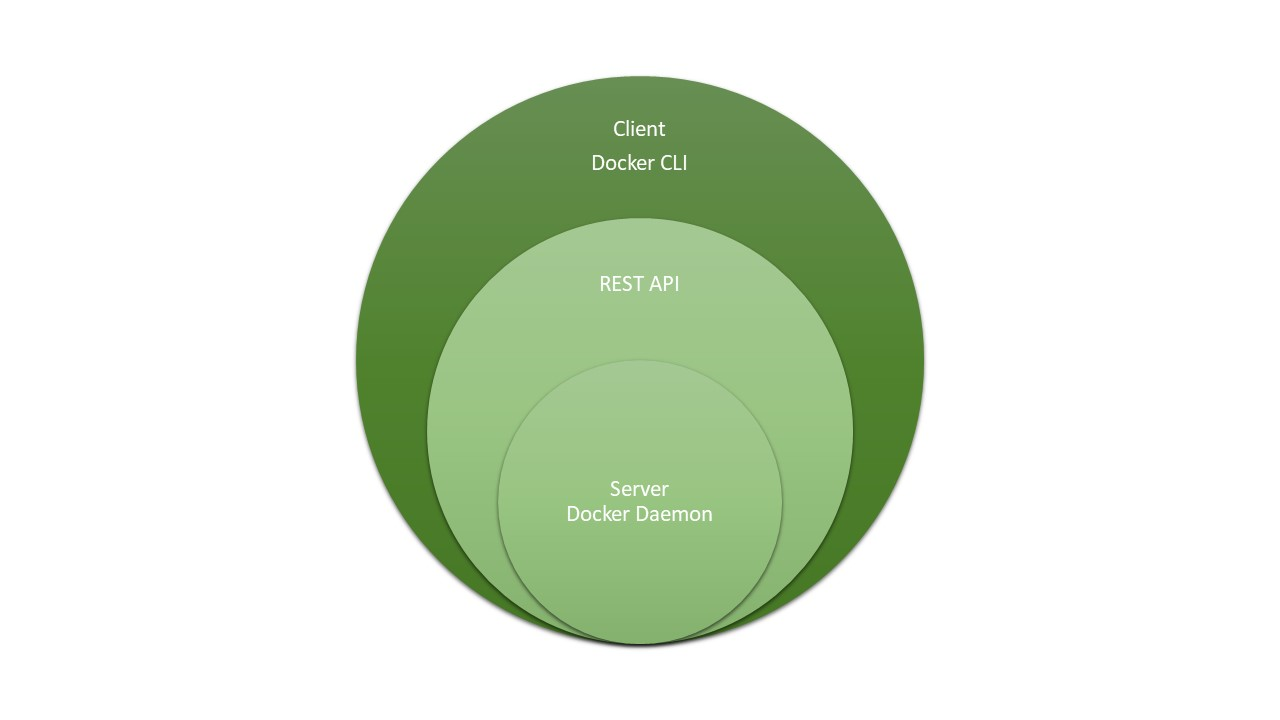
\includegraphics[width=0.7\textwidth]{images/docker_architecture.jpg}
    \caption[Docker Architektur]{Docker Architektur}
    \label{fig:Docker Architektur}
\end{figure}


Der Docker Client muss nicht zwingend auf dem Host-System laufen.
\footnote{Docker overview, vgl.~\cite{DOCKER_OVERVIEW}}

Es ist sogar möglich den Docker Socket in einen weiteren Container zu mounten und die Docker CLI innerhalb eines Containers zu verwenden, um Container auf dem Host-System zu verwalten.
\footnote{Singh et al., vgl.~\cite{Singh2017}~[S.806]}

% Über Client Zertifikatsauthentifizierung und HTTPS kann der Docker Client über das Internet verwendet werden, um einen Docker Host aus der Ferne zu verwalten.
% `(https://gist.github.com/kekru/974e40bb1cd4b947a53cca5ba4b0bbe5)`



% \subsubsection{Container vs VM}\label{containers_vs_vm}

Bei der Virtualisierung von Servern wird Hardware emuliert, um mehrere virtuelle Maschinen auf einem physikalischen Server auszuführen.
Diese Technologie ermöglicht eine bessere Ausnutzung von Hardware Ressourcen und wird in der IT-Industrie oft verwendet.
\footnote{Potdar et al., vgl.~\cite{Potdar2020}~[S.1419]}
Container stellen den nächsten Evolutionsschritt im Bereich der Virtualisierung dar.
Die Nachteile von Virtualisierung haben zu der Entwicklung von Containern geführt.
\footnote{Potdar et al., vgl.~\cite{Potdar2020}~[S.1419]}
Auch wenn VMs und Container verschiedene Probleme lösen sollen, so kann man diese folgendermaßen miteinander vergleichen:
\footnote{Potdar et al., vgl.~\cite{Potdar2020}~[S.1422]} \\

% https://www.tablesgenerator.com/

\begin{table}[H]
\centering
\begin{tabular}{|r|c|c|}
\hline
\multicolumn{1}{|c|}{} & \textbf{VM} & \textbf{Container} \\ \hline
\textbf{Isolation der Prozesse} & Auf Hardware Level & Auf Betriebssystem Level \\ \hline
\textbf{Betriebssystem} & Getrennt & Geteilt \\ \hline
\textbf{Startzeit} & Lang & Kurz \\ \hline
\textbf{Ressourcenverbrauch} & Mehr & Weniger \\ \hline
\textbf{Vorgefertigte Images} & Kaum verfügbar & Docker Registry \\ \hline
\textbf{Anpassbare Images} & Komplizierte Erstellung & Dockerfile \\ \hline
\textbf{Größe} & Größer (mit Betriebssystem) & Klein (nur Anwendung) \\ \hline
\textbf{Mobilität} & \begin{tabular}[c]{@{}c@{}}Einfach von einem Host zum \\ verschiebbar\end{tabular} & \begin{tabular}[c]{@{}c@{}}Container werden gelöscht\\ und neu erstellt.\end{tabular} \\ \hline
\textbf{Erstellungszeit} & Minuten & Sekunden \\ \hline
\end{tabular}
\caption{Container vs. VMs} \footnote{Pahl, vgl.~\cite{Pahl2015}~[S.25]}
\label{tab:container-vs-vm}
\end{table}

Tests haben gezeigt, dass Container in den meisten Fällen schneller sind als virtuelle Maschinen.
Container sind somit effizienter. \footnote{Potdar et al., vgl.~\cite{Potdar2020}~[S.1428]}


% IaC
\newpage
\subsection{Infrastructure as Code}\label{iac_basics}

Infrastructure as Code (IaC) bezeichnet die Verwendung von Praktiken aus der Softwareentwicklung bei der Verwaltung von Servern und anderer IT-Infrastruktur.
\footnote{Siebra et al., vgl.~\cite{Siebra2019}~[S.428]}
\footnote{Artac et al., vgl.~\cite{Artac2017}~[S.497]}

IaC soll die Verwaltung von Infrastruktur automatisierbar machen.
Sich wiederholende Aufgaben und manuelle Konfiguration sollen so minimiert werden.
\footnote{Siebra et al., vgl.~\cite{Siebra2019}~[S.428 - S.429]}

Für das DevOps \textbf{CAMS} ist IaC das A für Automatisierung.
Ohne IaC lässt sich keine Automatisierung erreichen und IaC ist somit essenziell für CI/CD und DevOps.
% `(Johann, 117)`
\footnote{Rahman, vgl.~\cite{Rahman2018c}~[S.476]} \\

Die IT-Industrie ist für eine hohe Innovationsgeschwindigkeit bekannt.
IaC soll es Entwicklern ermöglichen, Infrastruktur selbst zur Verfügung zu stellen.
Darüber hinaus wird dadurch eine höhere Entwicklungsgeschwindigkeit und schnellere Releases ermöglicht.
\footnote{Guerriero et al., vgl.~\cite{Guerriero2019}~[S.580]}
\footnote{Artac et al., vgl.~\cite{Artac2017}~[S.497]}

\subsubsection{Vorteile}\label{iac_vorteile}

In der Literatur finden sich folgende positiven Aspekte für den Einsatz von IaC:
\footnote{Siebra et al., vgl.~\cite{Siebra2019}~[S.428]}
% `(Johann, 118-120)`
\footnote{Artac et al., vgl.~\cite{Artac2017}~[S.497]}

\begin{itemize}
    \item \textbf{Dokumentation:}
    Durch die IaC Skripte ist dokumentiert, wie die Infrastruktur konfiguriert ist.

    \item \textbf{Versionierung:}
    Die Änderungshistorie und verschiedene Versionen sind durch den Einsatz von z.B. Git immer verfügbar.

    \item \textbf{Wiederholbarkeit:}
    IaC Skripte können immer wieder für verschiedene Umgebungen ausgeführt werden.
    Dadurch lassen sich Test-, Entwicklungs- und Produktivumgebungen so ähnlich wie möglich halten.

    \item \textbf{Change Management:}
    Durch die Verwaltung in Git und die jederzeitige Nachvollziehbarkeit ist es einfacher Änderungen an der Infrastruktur strukturiert durchzuführen.

    \item \textbf{Wiederherstellungsgeschwindigkeit:}
    Ein hoher Automatisierungsgrad erlaubt die schnelle Reaktion auf Fehlerfälle in dem z.B. die letzte Version wiederhergestellt oder ein Patch veröffentlicht wird.

    \item \textbf{Zuverlässigkeit:}
    Die Vermeidung von manueller Konfiguration führt zu weniger Fehlern und höherer Reproduzierbarkeit.

    \item \textbf{Auditierung:}
    Da alle Änderungen und die gesamte Konfiguration in Git erfasst sind, können Audits auf Basis dieser Informationen einfacher durchgeführt werden.

    \item \textbf{Massenoperationen:}
    Insbesondere, wenn eine Änderung auf vielen Servern gemacht werden soll, ist der Einsatz von IaC vorteilhaft.
\end{itemize}

\subsubsection{Herausforderungen}\label{iac_probleme}

Bezüglich der Herausforderungen, die der Einsatz von IaC mit sich bringen kann, werden die folgenden Aspekte hervorgehoben.
Die Schwierigkeiten wurden teilweise in einer Studie ermittelt, die verschiedene technische Mitarbeitern von einigen Unternehmen befragt hat:
\footnote{Guerriero et al., vgl.~\cite{Guerriero2019}~[S.580]}

\begin{itemize}
    \item \textbf{Verwaltung von Geheimnissen:}
    Dadurch dass IaC Skripte neben Passwörtern auch andere Geheimnisse enthalten können, hat jeder der Zugriff auf Git Repositories hat, ebenfalls Zugriff auf diese vertraulichen Daten.
    \footnote{Guerriero et al., vgl.~\cite{Guerriero2019}~[S.584]}

    \item \textbf{Testing:}
    Es gibt keine standardisierten Ansätze für das Testen von IaC Änderungen.
    Manchmal können Skripte nicht getestet werden, da diese unmittelbar, Änderungen im Produktivsystem durchführen.
    \footnote{Guerriero et al., vgl.~\cite{Guerriero2019}~[S.584]}

    \item \textbf{Modularisierung:}
    IaC ist keine Programmierung.
    Ansätze wie Modularisierung und Vererbung sind nicht immer verfügbar und führen zu vielen Wiederholungen in den Skripten.
    \footnote{Guerriero et al., vgl.~\cite{Guerriero2019}~[S.584]}

    \item \textbf{Unterschiedliche IaC Ansätze:}
    Es existiert eine Vielzahl von Tools, die unterschiedliche Ansätze verfolgen.
    Dies macht es manchmal notwendig, mehrere IaC Lösungen parallel zu nutzen.

    \item \textbf{Konsequenzen von Fehlern:}
    Ein unentdeckter Fehler in einem IaC Skript kann fatale Konsequenzen haben.
    So wurde 2017 auf über 270 Servern von Wikimedia das Home Verzeichnis gelöscht, was zu einem Ausfall führte.
    GitHub hatte einen Ausfall, weil ein DNS-Eintrag entfernt wurde. \footnote{Rahaman, vgl.~\cite{Rahman2018b}~[S.476]}
    \footnote{Rahaman et al., vgl.~\cite{Rahman2018}~[S.2]}

    \item \textbf{Lange Feedback Loops:}
    Das Erstellen von Infrastruktur ist zeitaufwändiger als das bloße Kompilieren von Quellcode.
    Ein Entwickler muss also länger warten bevor dieser Feedback zu einer IaC Änderung erhält.
    \footnote{Guerriero et al., vgl.~\cite{Guerriero2019}~[S.583]}

\end{itemize}

\subsubsection{Arten von IaC}\label{iac_arten}

IaC ist ein Sammelbegriff für Tools, die es erlauben Konfiguration und Provisionierung von Infrastruktur in Dateien zu erfassen und auszuführen.
Die Ansätze der verschiedenen Ausprägungen von Tools sind jedoch unterschiedlich.
Dieser Abschnitt beschreibt die gängigen Ansätze.
\footnote{Guerriero et al., vgl.~\cite{Guerriero2019}~[S.581]}

\paragraph{Ad-Hoc Skripte}

Ad-Hoc Skripte stellen  den ersten Schritt zur Einführung von IaC dar.
Hierbei handelt es sich um das Skripting von Schritten, die sonst manuell ausgeführt werden würden.
Wenn der Administrator z.B. eine bestimmte Auswahl von Kommandos zur Installation bzw. Konfiguration in einem Skript erfasst, ist das bereits der erste Schritt zu IaC.
Diese Skripte können dann ausgeführt werden, um bestimmte Aufgaben zu automatisieren.
Die schnellere Erledigung von Aufgaben kann somit Zeit sparen.
% `(Johann, 118)`

\paragraph{Configuration Management Tools}

Bei Configuration Management Tools (CM) handelt es sich um Software, die es ermöglicht bereits vorhandene Infrastruktur zu verwalten.
\footnote{Siebra et al., vgl.~\cite{Siebra2019}~[S.428]}

Auch die Installation neuer Systeme kann mit CM Software durchgeführt werden.
Der Fokus liegt jedoch meistens auf der Verwaltung bestehender Systeme.
Bekannte Tools sind hier Chef, Ansible und Puppet.

Die Abgrenzung zwischen CM und Provisionierung ist nicht immer ganz klar.
Diese Tools fokussieren sich aber eher darauf, mehrere Server gleichzeitig verwalten zu können.
Tools wie Ansible können z.B. Konfigurationsänderungen und neue Software auf vielen Systemen gleichzeitig ausrollen.

\paragraph{Server Templating Tools}

Diese Tools zielen darauf ab, beim Aufsetzen neuer Server auf Images oder Templates zurückgreifen zu können.
Ein bekanntes Tool ist Packer, womit sich Server konfigurieren lassen.
Per Skript kann dann die Software darauf installiert sowie konfiguriert werden und anschließend wird daraus ein Image erstellt.
\footnote{Packer - Build automated machine images, vgl.~\cite{PACKER}}

Packer unterstützt beispielsweise die Maschinen Image Formate von Azure, AWS, VmWare und Google Cloud.
Sobald ein Image einmal erstellt wurde, kann es von anderen Arten von IaC Tools ebenfalls verwendet werden.

\paragraph{Server Provisioning Tools}

Diese Art von IaC rückt die Erstellung und Konfiguration von Cloud Infrastruktur in den Vordergrund.
Solche Tools sind durch den Trend zu Cloud Computing beliebt geworden.
Sie vermeiden, dass man sich durch die Dialoge und Menüs der einzelnen Cloud-Provider durchklicken muss. \\

Mit Server Provisioning Tools geht man eher dazu über, die \textsl{Server wie Vieh und nicht wie Haustiere zu behandeln}.
% `(Johann, 117)`
Dieser Ansatz meint, dass Server eher neuaufgesetzt werden, als bestehende Server zu pflegen.
Durch hohe Automatisierung und theoretisch unbegrenzte Kapazitäten in der Cloud können Server so kontinuierlich ersetzt werden.
Ein Server, der sich nicht mehr korrekt verhält, wird einfach durch einen neuen ersetzt.

%    [RESTE]
%    - IaC essential to CI/CD,  IaC helps software teams with automation and deploying changes rapidly, IaC is Growing in popularity `(Rahaman, Partho, Morrison, 1)`
%    - The DevOps methodology is radically changing the way software is designed and managed nowadays. `(Guerriero, 581)`
%    - IT organizations that have adopted DevOps have strong collabora- tion between software development and operations teams to deliver software rapidly [8]. Automation of development and deployment steps is key to DevOps adoption, and DevOps organizations use technologies to automate repetitive work [8]. `(Rahman, 476)`
%    - The current IT market is increasingly dominated by the “need for speed” `(Artac, 497)`
%    - “need for speed": speed in deployment, faster release-cycles, speed in recovery, and more `(Guerriero, 580)`
%    - Infrastructure as Code (IaC) is a DevOps principle used to address problems regarding the manual process of configuration management by means of automatic provision and configuration of infrastructural resources `(Siebra, 428)`
%    - The goal is, essentially, to be able to survive as an organization in the modern digital ecosystem and digital market, which demands for fast and early releases, continuous software updates, constant evolution of market needs, and adoption of scalable technologies such as Cloud computing `(Guerriero, 581)`
%    - Kief Morris: "Treat your servers as cattle, not as pets" `(Johann, 117)`
%    - IaC ist das A in CAMS - Automatisierung `(Johann, 117)`
%    - IaC scripts help to provision and manage cloud-based infrastructure [8] `(Rahman, 476)`
%    - IaC is the technology of automatically defining and managing computing and network configurations, and infrastructure through source code `(Rahman, 477)`
%    - entail re-using standard tools from software development (e.g., code-versioning, code- revision management, etc.) to manage what is known as infrastructure-as-code (IasC) [2]. `(Artac, 497)`
%    - IasC is a key enabler of several DevOps tenets that heavily depend on automation. `(Artac, 497)`
%    - The philosophy behind this is that infrastructure has become like data `(Johann, 117)`
%    - bring in best prac- tices from software development, such as continuous integration [CI], test-driven development, and continuous delivery [CD] version control systems, and apply them to managing our infrastructure `(Johann, 117)`
%    - Cloud platforms have API to manage cloud ressources `(Johann, 117)`
%    - With CFEngine, you defined what you wanted your infrastructure to be [with code] in fi les, and then the tool applied [the code] to make it so on your infrastructure, and to make it continuously so `(Johann, 118)`
%    - "Iron Age" vs "Cloud Age": Physical infrastructure vs virtual infrustructure `(Johann, 118)`
%    - Benefits: Testings, Versioning, mass updates, tracing/auditing, catch mistakes early, reproducible infrastructure `(Johann, 118-120)`
%    - practitioners identify testability, readability, consistency, and portability as major technical challenges which still need much attention from the state of the art and practice `(Guerriero, 580)`
%    - Currently, the landscape of IaC languages and tools is jeopardized by the technology heterogeneity and by the huge number of available solutions, it complicates the understanding and adoption of this new technology `(Guerriero, 581)`
%    - Difference between standard code and IaC code by number of mentions in the answers:  `(Guerriero, 583)`
%    - Impossible Testing (8) - The lack of standard practices for testing and proper (maybe local) testing environments makes testing painful
%    - Declarative (7) - Standard programming is in terms of class, functions, flow. With IaC the reasoning is declarative, i.e., express what is needed, not how to do it.
%    - Graph vs. Tree model (7) - Production code is shaped as a graph of modules whereas IaC code resembles a tree of nodes
%    - Impossible Debugging (6) - Similar to testing, the lack of standard practices and the distributed nature makes debugging painful.
%    - IaC error-prone (5) - The tools for code checking are more shallow for IaC (e.g., lack of type-checking).
%    - Longer feedback loop (3) - The developer has to wait for the whole infrastructure to be deployed in order to understand the correctness of the IaC code.
%    - Unmaintainable (2) - As the infrastructure evolves and the computer resources changes, IaC code cannot cope with those on a seamless way.
%    - Bad practices when developing IaC Code `(Guerriero, 584)`
%    - Hardcoding (5) - Hardcoding values on the script such as credential or constants.
%    - Too Polyglot (4) - Using many languages in interrelated node definitions
%    - Blob blueprints (3) - Generating too large scripts.
%    - Non idempotent code (3) - Writing scripts with side effects can lead to undesired states.
%    - Poor documenting (3) - Hinders understandability and maintainability
%    - Manual infrastructure (2) - Some parts of the configuration are made manually, outside of IaC scripts.
%    - Nodes too deep (2) - The tree of nodes generated from a single script is too deep.
%    - Best practices when developing IaC Code `(Guerriero, 584)`
%    - Secret-Injection (12) - Keep all contents of the blueprint or IaC scripts parametric so that the orchestrator or users can inject the desired results at will
%    - Break-fast (8) - program the infrastructure to be buildable as fast as possible and hopefully as fast-breaking as possible furthermore, infrastructure circuit-breakers are needed to minimize waste
%    - Reuse by Abstraction (6) - Making templates and scripts also recall each-other to allow for interdependency but also interchangeability and possibly reuse, e.g., object orientation
%    - Low-Nesting (5) - Keep nodes nesting to at most one level of recall (i.e., tree of height 2)
%    - There does not exist one full-fledged and bullet-proof solution for IaC, rather the tools used by practitioners are very varied and also very common
%    - Defects in infrastructure as code (IaC) scripts can have serious consequences for organizations who adopt DevOps. `(Rahman, 476)`
%    - January 2017, execution of a defective IaC script erased home directories of 270 users in cloud instances maintained by Wikimedia `(Rahman, 476)`
%    - IaC scripts can also contain defects, metrics and static code analysis can help to prevent outages (like Github had DNS outage due to a wrong IaC) `(Rahaman, Stallings, Williams, 2)`
%    - Benefits from IaC `(Siebra, 428)`
%    - Code can be thoroughly tested to reproduce infrastructure consistently at scale
%    - Developers could be provided with a simulated production environment, which increases testability and reliability
%    - Infrastructure code can be versioned
%    - Infrastructure can be provisioned and configured on demand
%    - Proactive recovering from failures can be carried out by continuous monitoring of the environment for violations, which can trigger automatic execution of scripts for rollback or recovery.
%    - Patterns to use the infrastructure as code were proposed in (Duvall, 2011) and they can be summarized as: `(Siebra, 428-429)`
%    - Automate Provisioning
%    - Behavior-Driven Monitoring: automate tests to verify the behavior of the infrastructure
%    - Immune System: deploy software one instance at a time while conducting behavior-driven monitoring
%    - Lockdown Environments: lock down shared environments from unauthorized external and internal usage
%    - Production-Like Environments: development and production environments must be as similar as possible
%    - Shell scripts are potentially complex to maintain and evolve, since they are neither modular nor reusable `(Siebra, 430)`
%    - “Build incrementally with fast integrated learning cycles”.  `(Siebra, 430)`
%    - Patterns to use the infrastructure as code were proposed in (Duvall, 2011) and they can be summarized as: `(Siebra, 428-429)`
%    - Automate Provisioning
%    - Behavior-Driven Monitoring: automate tests to verify the behavior of the infrastructure
%    - Immune System: deploy software one instance at a time while conducting behavior-driven monitoring
%    - Lockdown Environments: lock down shared environments from unauthorized external and internal usage
%    - Production-Like Environments: development and production environments must be as similar as possible

\newpage

% Evaluierung der Tools
\fancyhead[L]{\nouppercase{Evaluierung}}
\section{Evaluierung der Tools}\label{evaluierung}

Zu den Bestandteilen einer CI/CD-Pipeline für DevOps gehören ein Versionskontrollsystem (VCS idealerweise mit integrierten Kollaborationstools),
ein CI Server, IaC Skript und eine Zielumgebung für das Deployment.
\footnote{Rahman, vgl.~\cite{Rahman2018c}~[S.477]} \\

In den kommenden Abschnitten werden zunächst gängige Tools ermittelt und anschließend miteinander verglichen.

Die Auswahl der zu evaluierenden Tools erfolgt dabei auf Basis einer Auswertung der auf Stackshare geteilten Technologiestacks.
Hierfür werden vor allem kostenlos nutzbare Tools bevorzugt. \\

Stackshare wurde im Jahre 2014 gegründet und verfolgt das Ziel, die eingesetzten Technologien von Unternehmen zu sammeln.
\footnote{www.stackshare.io, vgl.~\cite{STACKSHARE_HOME}}

Bereits 2017 hatten dort ca. 7000 Unternehmen ihre eingesetzten Technolgien hintgerlegt.
Darunter auch Unternehmen wie AirBnb, Pintrest, Uber, Facebook und Google.
Mittlerweile haben dort über 150.000 Entwickler und Unternehmen ihre Stacks geteilt.

Aus den dort hinterlegten Technologien lässt sich eine Liste über die Beliebtheit der verschiedener Tools ermitteln.
\footnote{Techcrunch, vgl.~\cite{TECHCRUNCH_STACKSHARE}}
\subsection{Kollaboration und Versionskontrolle}\label{collaboration_vcs}

Tools für die Versionskontrolle benötigen immer auch eine serverseitige Lösung, um die Zusammenarbeit zwischen Entwicklern zu ermöglichen.
Neben Git gibt es für die Versionskontrolle einige Alternative.
Aufgrund des weitaus geringeren Marktanteils dieser Alternativen fällt deren Betrachtung in dieser Arbeit weg.
\footnote{What are the best Version Control System Tools?, vgl.~\cite{STACKSHARE_VCS}}

Bei Stackshare werden in dieser Kategorie folgende Tools aufgeführt:
\footnote{What are the best Code Collaboration and Version Control Tools?, vgl.~\cite{STACKSHARE_CODE_COLLABORATION}}

\begin{itemize}
    \item \textbf{GitHub:} \href{https://github.com/}{https://github.com/}
    \item \textbf{GitLab:} \href{https://about.gitlab.com/}{https://about.gitlab.com/}
    \item \textbf{Atlassian Bitbucket:} \href{https://bitbucket.org/}{https://bitbucket.org/}
    \item \textbf{AWS CodeCommit:} \href{https://aws.amazon.com/codecommit}{https://aws.amazon.com/codecommit}
\end{itemize}


%\footnote{GitHub Pricing, vgl.~\cite{GITHUB_PRICING}}
%\footnote{GitHub free for all teams, vgl.~\cite{TECHCRUNCH_GITHUB_FREE}}
%
%\footnote{GitLab - Feature Comparison, vgl.~\cite{GITLAB_FEATURES}}
%\footnote{Bitbucket - Pricing, vgl.~\cite{BITBUCKET_PRICING}}
%\footnote{AWS CodeCommit Pricing, vgl.~\cite{AWS_CODECOMMIT_PRICING}}

%    - Pricing:
%    - Github `(https://github.com/pricing)`:
%    - Free `(https://techcrunch.com/2020/04/14/github-is-now-free-for-all-teams/)`:
%    - Unlimited public/private, collaborators
%    - 2000 Actions minutes/month
%    - 500 MB Package storage space
%    - Community support
%    - Team ($4 user/month):
%    - Unlimited public/private, collaborators
%    - Setup required reviewers
%    - 3000 Actions minutes/month
%    - 2 GB Package storage space
%    - Code owners
%    - Enterprise ($21 user/month):
%    - SAML - Single sign on
%    - 50.000 Actions minutes/month
%    - 50 GB Package storage space
%    - Advanced auditing
%    - GitHub One (Contact sales, unknown price):
%    Container vs. VMs      - 24/7 support
%    - Actionable metrics
%    - Gitlab `(https://about.gitlab.com/pricing/) and (https://about.gitlab.com/pricing/gitlab-com/feature-comparison/)`:
%    - Free:
%    - Unlimited public/private, collaborators (10 GB Limit total)
%    - 400 CI/CD minutes/month
%    - Own production environment/CI runners
%    - Bronze ($4 user/month):
%    - Single Team Project Management
%    - NBD support
%    - 2000 CI/CD minutes/month
%    - Sort issues, Scrum Charts, Multiple approvers, Push rules
%    - Silver ($19 user/month):
%    - Cross team project management, multiple approval roles, bulk edit issues, epics, roadmaps, approval rules for code review, audit events, deploy boards
%    - 10000 CI/CD minutes/month
%    - Priority support
%    - Gold ($99 user/month):
%    - Compliance automation, Advanced application security, Executive level insights, Create Test Cases, Secret Detection, Dependency scanning, Security Dashboards/Approvals, License Comliance
%    - 50000 CI/CD minutes/month
%    - Bitbucket `(https://www.atlassian.com/software/bitbucket/pricing)`:
%    - Free ($0 Up to 5 Users)
%    - 50 CI/CD minutes/month
%    - Jira/Trello integration
%    - 1 GB Git LFS Storage
%    - Standard ($3 user/month)
%    - 2500 CI/CD minutes/month
%    - 5 GB Git LFS Storage
%    - Premium ($6 user/month)
%    - 3500 CI/CD minutes/month
%    - 10 GB Git LFS Storage
%    - AWS Code Commit `(https://aws.amazon.com/de/codecommit/pricing/)`:
%    - Free ($0 Up to 5 Users)
%    - Unlimited Repos
%    - 50 GB Storage
%    - 10.000 Git Request/Month
%    - After 5 Users ($1 per additional user/month)
%    - 10 GB per User
%    - 2.000 Git Request/Month per User
%    - "Pay-as-you-go" General pricing after limits are reached
%    - 0,06 USD pro GB und Monat
%    - 0,001 USD pro Git-Anfrage
%    - Commercial support:
%    - Github `(https://github.com/premium-support)`:
%    - Yes, starting with Enterprise Level
%    - GitLab: `(https://about.gitlab.com/support/)`
%    - Starting with Bronze, Priority Support for higher plans included.
%    - BitBucket: `(https://confluence.atlassian.com/support/atlassian-support-offerings-193299636.html)`
%    - Starting with Standard Plan (9/5), Premium (24/7)
%    - AWS Code Commit: `(https://aws.amazon.com/de/premiumsupport/pricing/)`
%    - Through AWS support $ 29 or 3% of monthly bill
%
%    - Private Repos:
%    - Github: Unlimited
%    - GitLab: Unlimited
%    - BitBucket: Unlimited
%    - AWS Code Commit: Unlimited
%
%    - Self Hosting possible:
%    - Github: Yes, no pricing without contacting sales `(https://github.com/enterprise)`
%    - GitLab: Yes, even for free `(https://about.gitlab.com/install/)`
%    - BitBucket: Yes, but no new licenses starting Feb 2021, EOL Feb. 2024 `(https://bitbucket.org/product/enterprise)`
%    - AWS Code Commit: No
%
%    - Issue Tracker:
%    - Github: Yes
%    - GitLab: Yes
%    - BitBucket: Through Jira Connection
%    - AWS Code Commit: No
%
%    - Ticket System:
%    - Github: Only issues
%    - GitLab: Yes
%    - BitBucket: Jira
%    - AWS Code Commit: No
%
%    - Authentication Methods:
%    - Github: Email/Password, LDAP only for Enterprise
%    - GitLab: Email/Password, LDAP (Self Hosted, Bronze), Google, Github, Twitter, Bitbucket, Salesforce
%    - BitBucket: Email/Password
%    - AWS Code Commit: IAM
%
%    - MFA
%    - Github: Yes
%    - GitLab: Yes
%    - BitBucket: Yes
%    - AWS Code Commit: Through IAM
%
%    - Permissions:
%    - Github: On repository level: Collaborators can be defined
%    - GitLab: On repository and group level: Users with differnet roles from Maintainer, Developer, Reporter to Guest
%    - BitBucket: On account, repository and even branch level, groups (Read/Write/Admin), Guest users and invitations
%    - AWS Code Commit: Through IAM
%
%    - Protected branches:
%    - Github: Yes with wildcards
%    - GitLab: Yes with wildcards
%    - BitBucket: Yes, with wildcards and through permissions
%    - AWS Code Commit: Yes with wildcards
%
%    - Web based code editor:
%    - Github: Yes
%    - GitLab: Yes
%    - BitBucket: Yes
%    - AWS Code Commit: Yes (but ugly) => Cloud 9 Part of AWS but extra pricing
%
%    - Web based code review:
%    - Github: Yes
%    - GitLab: Yes
%    - BitBucket: Yes
%    - AWS Code Commit: Yes
%
%    - Web based code approval:
%    - Github: Yes, with rules
%    - GitLab: Yes (starting with Bronze plan)
%    - BitBucket:
%    - AWS Code Commit
%
%    - LFS Support:
%    - Github: Yes
%    - GitLab: Yes
%    - BitBucket: Yes
%    - AWS Code Commit: Yes
%
%    - Support für Wikis/Dokumentation:
%    - Github: Yes
%    - GitLab: Yes
%    - BitBucket: No
%    - AWS Code Commit: No
%
%    - Statistiken:
%    - Github: Yes, through Insights
%    - GitLab: Yes, through Analytics
%    - BitBucket: No, but available when Jira is connected
%    - AWS Code Commit: Yes, through CloudWatch, CloudTrail and EventBridge, manual setup needed
%
%    - CI/CD integrated:
%    - Github: Yes, GitHub Actions
%    - GitLab: Yes, GitLab Runner
%    - BitBucket: Yes, Pipelines
%    - AWS Code Commit: Yes, AWS CodeBuild
%
%    - Vulnerability Scans:
%    - Github: Yes
%    - GitLab: Yes, staring with
%    - BitBucket: No
%    - AWS Code Commit: No
%
%    - Platform specials:
%    - Github: GitHub Desktop: https://desktop.github.com/
%    - GitLab: Jira Like
%    - BitBucket: SourceTree Git Client for Windows/MacOS
%    - AWS Code Commit: Pay as you go pricing, Part of CodeStar (Code Guru for Java/Python)
%
%    - Rank on stackshare:
%    - Github: 1. 132.000 Stacks / 4. 465 Stacks
%    - GitLab: 2. 30.500 Stacks
%    - BitBucket: 3. 25.800 Stacks
%    - AWS Code Commit: 4. 243 Stacks
%
%
%    ​








\newpage
\subsubsection{Auswahlkriterien}\label{collaboration_vcs_kriterien}

Zur Auswahl des Tools werden die folgenden Fragestellungen beantwortet:

\begin{itemize}
    \item \textbf{Unterstützung Privater Repositories:}
    Erlaubt das Tool private Repositories zu verwalten, die nicht öffentlich einsehbar sind?

    \item \textbf{Authentifizierungsmethoden:}
    Gerade im Unternehmensumfeld sind LDAP Integration oder andere Methoden wünschenswert.
    Welche Methoden für Authentifizierung und Autorisierung werden unterstützt?

    \item \textbf{Issue Tracker/Ticket System:}
    Unterstützt das Tool die Erstellung von Tickets und kann es diese in Boards verwalten?
    Tools mit einem Ticket System können ggf. direkt auch für die Planung von Meilensteinen und Scrum verwendet werden.

    \item \textbf{Code Editor:}
    Kann Quellcode direkt über die Web UI bearbeitet werden?

    \item \textbf{Code Review Unterstützung:}
    Lassen sich Merge Requests erstellen und über die Weboberfläche bearbeiten?
    
    \item \textbf{Code Review Approvals:}
    Können mehrere Personen einen Code Review durchführen, sodass dieser erst nach Bestätigung von mehreren Personen akzeptiert werden kann?

    \item \textbf{CI/CD Integration:}
    Ist ein Tool für die Verwaltung von CI/CD Pipelines integriert?

    \item \textbf{Self Hosting:}
    Kann das Tool \textsl{On-Premise} bzw. auf eigenen Servern installiert werden?

    \item \textbf{Kommerzieller Support:}
    Gibt es eine kommerzielle Version oder Support für Unternehmen?

    \item \textbf{Statistiken:}
    Unterstützt das Tool die Erfassung von Statistiken und Metriken zu den Aktivitäten?

    \item \textbf{Kosten:}
    Wie ist die Preisgestaltung?

    \item \textbf{Rang auf Stackshare:}
    Welchen Rang und wieviel Stacks hat das Tool auf Stackshare?
\end{itemize}
\newpage
\subsubsection{Tools}\label{collaboration_vcs_tools}

\paragraph{GitHub}\label{collaboration_github}

GitHub wurde 2008 als erste kommerzielle Hosted Git Software gestartet \footnote{Medium.com, vgl.~\cite{GITHUB_STORY}}
und im Oktober von 2018 für 7,5 Milliarden Dollar von Microsoft übernommen. \footnote{theverge.com, vgl.~\cite{GITHUB_MICROSOFT}}
Mit mehr als 56 Millionen Entwicklern, über 3 Millionen Organisationen und mehr als 100 Millionen Repositories ist GitHub
weltweit die größe Hosted Git Platform.
Darüber hinaus setzen 72\% der Fortune 50 Unternehmen GitHub ein. \footnote{Github Website, vgl.~\cite{GITHUB_HOME}} \\

GitHub ist kostenlos nutzbar.
Dabei kann eine unbegrenzte Anzahl öffentlicher und privater Repositories angelegt werden.
Die Kommunikation zwischen den Entwicklern erfolgt über Issues.
Als CI/CD Pipeline kann GitHub Actions verwendet werden, andere CI/CD Tools unterstützen jedoch eine Einbindung von GitHub,
da der überwiegende Teil der Open Source Landschaft GitHub verwendet. \\

Zu den Besonderheiten von GitHub gehören die Unterstützung von statischen Websites (GitHub Pages), Wikis und
automatisierte Scans nach Sicherheitslücken in den verwendeten Abhängigkeiten von Projekten auf GitHub.



\paragraph{GitLab}\label{collaboration_gitlab}

GitLab wurde 2013 als Open-Source Software für die Installation auf dem eigenen Server gestartet. \footnote{thenextweb.com, vgl.~\cite{GITLAB_ANOUNCMENT}}
Die Lösung ist dreigeteilt in eine gehostete Version, eine kommerzielle und eine Open-Source Version. \footnote{GitLab Website, vgl.~\cite{GITLAB_ABOUT}}
Laut eigenen Angaben verwenden ca.
30 Millionen Entwickler und 100.000 Organisationen GitLab.
GitLab ist vor allem als selbsgehosteter Git Server beliebt, da sich die Open-Source Version auch für Unternehmen kostenlos nutzen lässt. \footnote{GitLab Pricing, vgl.~\cite{GITLAB_PRICING}}

Die kostenlose Version von GitLab hat bereits einen Funktionsumfang, der für kleine bis mittlere Unternehmen ausreichend ist.
Es lassen sich hier auch Kanban Boards, Milestones und das Ticket System nutzen.
GitLab stellt eine DevOps-Platform dar bei der auch mit GitLab Runner ein CI/CD System integriert.
\paragraph{Bitbucket}\label{collaboration_bitbucket}

Bitbucket wurde 2008 für das Mercurial VCS gestartet und dabei auf einer Mercurial Mailing Liste angekündigt. \footnote{Announcement in Mercurial Mailing List, vgl.~\cite{BITBUCKET_HISTORY}}
Im Jahr 2010 wurde BitBucket dann von Atlassian übernommen.
Atlassian verfügt über ein umfangreiches Portfolio von Entwicklertools.
Neben Ticketsystemen wie Jira, Kollaborationswerkzeugen Confluence und Trello gehören auf DevOps Tools wie BitBucket, SourceTree sowie Bamboo zum Portfolio des Unternehmens. \footnote{Atlassian Products, vgl.~\cite{BITBUCKET_OTHER_PRODUCTS}}

Jira Tickets lassen sich in BitBucket integrieren und auch BitBucket bietet einen eigenen CI/CD Dienst an.
\paragraph{AWS CodeCommit}\label{collaboration_aws_code_commit}

AWS hat 2015 verschiedene Tools für DevOps veröffentlicht.
Darunter auch AWS-Code-Commit.
Es handelt sich dabei um ein vollständig von AWS verwaltetes hosted Git, dass den bei Amazon üblichen \textsl{Pay per Use} Ansatz verfolgt.
\footnote{AWS News Blog - Code Commit, vgl.~\cite{AWS_CODECOMMIT_ANOUNCEMENT}} \\

Die weiteren Produkte für DevOps werden als AWS CodeStar bezeichnet und enthalten Werkzeuge für die Implemetierung von CI/CD Pipelines, die in die anderen AWS Dienste integriert sind.
\footnote{AWS News Blog - Tools for Code Management, vgl.~\cite{AWS_CODESTAR_ANOUNCEMENT}}
AWS CodeStar bietet dabei alles an, was für die Implementierung einer CI/CD Pipeline in AWS notwendig ist. \footnote{AWS Developer Tools Documentation, vgl.~\cite{AWS_DEVELOPER_TOOLS}}
Mit der Übernahme von Cloud 9 im Jahr 2016 bietet AWS auch eine webbasierte IDE an. \footnote{AWS Cloud 9, vgl.~\cite{AWS_CLOUD9}}

\newpage
\subsubsection{Vergleich}\label{collaboration_vcs_vergleich}

% Please add the following required packages to your document preamble:
% \usepackage{multirow}
% \usepackage{graphicx}
\begin{table}[H]
\centering
\resizebox{\textwidth}{!}{%
\begin{tabular}{r|c|c|c|c|}
\cline{2-5}
\multicolumn{1}{l|}{} & \textbf{GitHub} & \textbf{GitLab} & \textbf{BitBucket} & \textbf{AWS CodeCommit} \\ \hline
\multicolumn{1}{|r|}{\textbf{Private Repositories}} & ja (unbegrenzt) & ja (unbegrenzt) & ja (unbegrenzt) & ja (unbegrenzt) \\ \hline
\multicolumn{1}{|r|}{\textbf{Authentifizierungsmethoden}} & \begin{tabular}[c]{@{}c@{}}Email,\\ LDAP (Enterprise)\end{tabular} & \begin{tabular}[c]{@{}c@{}}Email, Google,\\ Github, LDAP,\\ Twitter, Bitbucket,\\ Salesforce\end{tabular} & Email & IAM \\ \hline
\multicolumn{1}{|r|}{\textbf{Issue Tracker / Ticket System}} & Nur Issues & Komplettes Ticketsystem & \begin{tabular}[c]{@{}c@{}}Nur über\\ Jira Integration\end{tabular} & Nein \\ \hline
\multicolumn{1}{|r|}{\textbf{Code Editor}} & Ja & Ja & Ja & Ja \\ \hline
\multicolumn{1}{|r|}{\textbf{Code Review Unterstützung}} & Ja & Ja & Ja & Ja (rudimentär) \\ \hline
\multicolumn{1}{|r|}{\textbf{Code Review Approvals}} & Ja & Ja (ab Bronze) & Ja (ab Premium) & Nein \\ \hline
\multicolumn{1}{|r|}{\textbf{CI/CD Integration}} & Ja, GitHub Actions & Ja, GitLab Runner & Ja & Ja, AWS CodeBuild \\ \hline
\multicolumn{1}{|r|}{\textbf{Self Hosting}} & \begin{tabular}[c]{@{}c@{}}Ja\\ (Preis nur auf Anfrage)\end{tabular} & Ja (kostenlos) & Ja (EOL Feb. 2024) & Nein \\ \hline
\multicolumn{1}{|r|}{\textbf{Kommerzieller Support}} & \begin{tabular}[c]{@{}c@{}}Ja\\ (ab Enterprise Level)\end{tabular} & Ja (ab Bronze) & Ja (ab Standard) & \begin{tabular}[c]{@{}c@{}}Ja, AWS Support\\ (\$29 oder 3\%\\ der AWS Rechnung)\end{tabular} \\ \hline
\multicolumn{1}{|r|}{\textbf{Statistiken}} & Ja (Insights) & Ja (Analytics) & Nein (nur Jira) & \begin{tabular}[c]{@{}c@{}}Ja\\ (CloudWatch Setup\\ erforderlich)\end{tabular} \\ \hline
\multicolumn{1}{|r|}{\multirow{4}{*}{\textbf{\begin{tabular}[c]{@{}r@{}}Kosten\\ (pro Monat)\end{tabular}}}} & \begin{tabular}[c]{@{}c@{}}kostenlos\\ 2000 CI Minuten\\ 500 MB Package\\ Storage\end{tabular} & \begin{tabular}[c]{@{}c@{}}kostenlos\\ 400 CI Minuten\\ 10 GB Speicherplatz\end{tabular} & \begin{tabular}[c]{@{}c@{}}kostenlos\\ 50 CI Minuten\\ 1 GB LFS\end{tabular} & \begin{tabular}[c]{@{}c@{}}kostenlos\\ für bis zu 5 Benutzer\\ 50 GB Storage\\ 10.000 Git Anfragen\end{tabular} \\ \cline{2-5}
\multicolumn{1}{|r|}{} & \begin{tabular}[c]{@{}c@{}}Team (\$4)\\ pro Benutzer\\ 3000 CI Minuten\\ 2 GB Package\\ Storage\end{tabular} & \begin{tabular}[c]{@{}c@{}}Bronze (\$4)\\ 2.000 CI Minuten\\ Scrum Charts\\ Issues sortieren\\ Push Regeln\\ Code Review Approvals\end{tabular} & \begin{tabular}[c]{@{}c@{}}Standard (\$3)\\ 2.500 CI Minuten\\ 5 GB LFS\end{tabular} & \begin{tabular}[c]{@{}c@{}}Nach 5 Benutzern\\ \$1 pro weiterem \\ Benutzer\\ 2.000 Anfragen\\ pro Benutzer\end{tabular} \\ \cline{2-5}
\multicolumn{1}{|r|}{} & \begin{tabular}[c]{@{}c@{}}Enterprise (\$21)\\ pro Benutzer\\ 50.000 CI Minuten\\ 50 GB Package Storage\end{tabular} & \begin{tabular}[c]{@{}c@{}}Silver (\$19)\\ 10.000 CI Minuten\\ Roadmaps\\ Project Management\\ Audit Events\\ Deploy Boards\\ Priority Support\end{tabular} & \begin{tabular}[c]{@{}c@{}}Premium (\$6)\\ 3.500 CI Minuten\\ 10 GB LFS\end{tabular} & \begin{tabular}[c]{@{}c@{}}\$0,06 pro GB\\ 0,001 pro Anfrage\end{tabular} \\ \cline{2-5}
\multicolumn{1}{|r|}{} & \begin{tabular}[c]{@{}c@{}}GitHub One\\ Preis nur auf Anfrage\end{tabular} & \begin{tabular}[c]{@{}c@{}}Gold (\$99)\\ 50.000 CI Minuten\\ Compliance Automatisierung\\ Security Scanning\\ License Compliance\end{tabular} &  &  \\ \hline
\multicolumn{1}{|r|}{\textbf{Rang auf Stackshare}} & 1. (132.000 Stacks) & 2. (30.500 Stacks) & 3. (25.800 Stacks) & 4. (243 Stacks) \\ \hline
\multicolumn{1}{|r|}{\textbf{Besonderheiten}} & \begin{tabular}[c]{@{}c@{}}GitHub Desktop App\\ GitHub Pages\\ Wikis\\ Vulnerability Scans\end{tabular} & \begin{tabular}[c]{@{}c@{}}Kanban Boards\\ Ticketsystem\\ Vulnerability Scans\end{tabular} & \begin{tabular}[c]{@{}c@{}}Jira Integration\\ Berechtigungen auf\\ Branches\end{tabular} & \begin{tabular}[c]{@{}c@{}}Integration in AWS\\ "Pay as you go"\end{tabular} \\ \hline
\end{tabular}%
}
\caption{Vergleich VCS Tools}
\label{tab:vcs_tools_vergleich}
\end{table}
\subsubsection{Zusammenfassung}\label{collaboration_vcs_zusammenfassung}

Die Grundfunktionalität jedes untersuchten VCS ist ähnlich.
Es lassen sich Remote Git Repositories erstellen und verwalten.
Alle Tools erlauben eine kostenlose Nutzung auch mit privaten Repositories.
Dabei unterscheiden sie sich je nach Tool entweder bei den verfügbaren Features
oder den Kapazitäten von CI Minuten für die Ausführung von Pipelines.

Die Weboberflächen von GitHub, GitLab und Bitbucket erlauben es, Code Reviews benutzerfreundlich durchzuführen.
Bei AWS-Code-Commit ist die Benutzererfahrung bei Merge Requests und Kommentaren deutlich eingeschränkter als bei den drei anderen VCS. \\

GitHub bietet mit GitHub Pages und Wikis die Möglichkeit, statische Websites direkt aus einem Repository heraus zu hosten.
Das kann für die Erstellung einer Dokumentationswebsite nützlich sein, da diese dann direkt zusammen mit dem Quellcode versioniert wird. \\

GitLab ist in der Starter Version bereits umfangreich nutzbar.
Das Feature von \textit{Code Approvals} wird aber erst bei der Bronze Version freigeschaltet.
Als Alleinstellungsmerkmal hat GitLab hier die Möglichkeit Tickets, Meilensteine und Kanban Boards zu verwalten. \\

BitBucket ist in der Grundversion ein reines Remote Git Repository.
Es fehlt ein Ticket/Issue System, dieses kann aber über die Anbindung von Jira realisiert werden.
Dafür fallen dann allerdings zusätzliche Kosten an. \\

Die CodeStar-Tools von AWS sind umfangreich und sollten es Unternehmen erlauben, jeden beliebigen Workflow abzubilden.
Der große Nachteil hierbei ist die komplexe Einrichtung.
Die vielfältigen Möglichkeiten sorgen dafür, dass die Benutzeroberfläche weit weniger benutzerfreundlich ist.
Mit Cloud 9 bietet AWS eine webbasierte IDE. \\

Den größten kostenlos nutzbaren Funktionsumfang für eine gehostete VCS-Lösung bietet hier GitHub.
Mit 2.000 CI Minuten bewegt sich das kostenlose Angebot in einem Bereich bei dem man bei GitLab bereits \$4 pro Benutzer bezahlen muss.
\footnote{GitLab Pricing, vgl.~\cite{GITLAB_PRICING}}

\newpage
\subsection{CI/CD Server und Dienste}\label{ci_services}

Für CI/CD wird immer ein Server bzw.
Dienst benötigt, dessen Aufgabe die Ausführung der Jobs ist.
Diese Jobs können auf unterschiedliche Arten gestartet werden.
Üblicherweise geschieht dies durch das Erstellen eines Merge Request, den Push von neuem Code oder der Annahme eines Merge Requests. \\

Bei Stackshare werden in dieser Kategorie folgende Tools aufgeführt:
\footnote{What are the best Continuous Integration Tools?, vgl.~\cite{STACKSHARE_CI}}

\begin{itemize}
    \item \textbf{Jenkins:} \href{https://www.jenkins.io/}{https://www.jenkins.io/}
    \item \textbf{Circle CI:} \href{http://circleci.com/}{http://circleci.com/}
    \item \textbf{Travis CI:} \href{https://travis-ci.com/}{https://travis-ci.com/}
    \item \textbf{GitHub Actions:} \href{https://github.com/features/actions}{https://github.com/features/actions}
    \item \textbf{GitLab CI:} \href{https://docs.gitlab.com/runner/}{https://docs.gitlab.com/runner/}
\end{itemize}



\subsubsection{Auswahlkriterien}\label{ci_services_kriterien}

Zur Auswahl des Tools werden die folgenden Fragestellungen beantwortet:

% `(https://www.altexsoft.com/blog/engineering/comparison-of-most-popular-continuous-integration-tools-jenkins-teamcity-bamboo-travis-ci-and-more/)`

\begin{itemize}
    \item \textbf{Unterstützte Kollaborationstools:}
    Welche Kollaborationstools können als Quelle für die CI/CD Pipeline verwendet werden?

    \item \textbf{Authentifizierung:}
    Welche Dienste werden zur Authentifizierung von Benutzern verwendet?

    \item \textbf{Pipelines as Code:}
    Können Pipelines als Skripte angelegt werden?
    Falls dies möglich ist, in welcher Programmiersprache?

    \item \textbf{Verwaltung von Secrets:}
    Wie werden Passwörter und andere geheime Informationen verwaltet, um diese in CI/CD Pipelines zu injizieren?

    \item \textbf{Unterstützte Programmiersprachen:}
    Für welche Programmiersprachen sind Vorlagen vorhanden?

    \item \textbf{Unterstützte Betriebssysteme:}
    Auf welchen Betriebssystemen können Pipelines ausgeführt werden?

    \item \textbf{Container support:}
    Werden Docker Container innerhalb der Pipelines unterstützt?

    \item \textbf{Usability:}
    Wie schnell lässt sich ohne Vorkenntnisse eine Build Pipeline einrichten und starten?

    \item \textbf{Self Hosting:}
    Besteht die Möglichkeit den CI/CD Dienst auf eigenen Servern zu betreiben?

    \item \textbf{Kosten:}
    Welche Kosten entstehen und wie ist das Preismodell?

    \item \textbf{Rang auf Stackshare:}
    Welchen Rang und wie viele Stacks hat das Tool auf Stackshare?

    \item \textbf{Besonderheiten:}
    Welche Besonderheiten hat der Dienst gegenüber anderen Diensten zu bieten?
\end{itemize}

\subsubsection{Tools}\label{ci_services_tools}

Die folgenden Tools werden auf Stackshare aufgeführt und nachfolgend genauer untersucht.

\paragraph{Jenkins}\label{ci_services_tools_jenkins}

Im Jahre 2007 erschien Jenkins als Hudson Open-Source Build Server und wurde später umbenannt. \footnote{Hudson Announcement, vgl.~\cite{JENKINS_ANOUNCEMENT}}
Dieser wurde mit Abstand der beliebteste Build Server.
Durch zahlreiche Plugins (> 1.500 Stück) lässt er sich für alle Einsatzzwecke anpassen. \footnote{Jenkins Awards, vgl.~\cite{JENKINS_AWARDS}}
Der Dienst wird i.d.R. als selbst gehosteter Server eingesetzt und hat eine Master/Slave Architektur.
Der Master kontrolliert die sogenannten Jenkins Agents auf denen die Builds ausgeführt werden.
Es lassen sich jedoch auch Builds auf dem Master ausführen. \\

Durch die Unterstützung von Docker basierenden Agents lässt sich jede Programmiersprache - für die es ein Docker-Image gibt - verwenden.
Jenkins Agents lassen sich entweder über SSH oder über einen Java basierten Jenkins Agent verwalten.
Dadurch ist es möglich Windows, Linux und MacOS zu verwenden. \\

Die Konfiguration kann entweder über die Jenkins Oberfläche oder über Jenkinsfiles erstellt werden.
Ein Jenkinsfile wird dabei in der Programmiersprache Groovy verfasst. \footnote{Pipeline Syntax, vgl.~\cite{JENKINS_JENKINSFILE}}

Um Passwörter und andere Geheimnisse in die Builds zu injizieren stehen Plugins zur Verfügung.
Diese sorgen ebenfalls dafür, dass injizierte Geheimnisse nicht in den Log Dateien der Builds sichtbar sind. \\

Da es sich um einen selbst gehosteten Buildsserver handelt, lassen sich die Kosten nicht pauschal bestimmen.
Die Verwaltung einer Jenkins Infrastruktur erfordert also eine Administration vom Unternehmen selbst.

\paragraph{Travis CI}\label{ci_services_tools_travis}

Travic CI wurde 2011 von einem Berliner Unternehmen als gehosteter Build Service gestartet. \footnote{Crunchbase Travic CI , vgl.~\cite{CRUNCHBASE_TRAVIS_CI}}
Es findet bei über 900.000 Projekten Verwendung und ermöglicht das kostenlose Bauen von Open-Source-Projekte. \footnote{Travis Homepage , vgl.~\cite{TRAVIS_HOMEPAGE}} \\

Travis CI steht als SaaS zur Verfügung.
Die Kollaborationstools GitHub, GitLab, Bitbucket und Assembla werden unterstützt.
Die Builds laufen immer in einem Docker Container, somit wird von Travis CI jede Programmiersprache - für die es Docker Images gibt - unterstützt.
Die Erstellung der Build Konfiguration erfolgt über eine YAML Datei und eine DSL.
Travis CI bietet Agents für die Ausführung von Builds auf Windows, Linux und MacOS. \\

Durch die Verfügbarkeit von Templates und einer im Vergleich zu Jenkins kleineren Dokumentation lassen sich
Builds schnell einrichten. \\

In der kostenlosen Version sind 10.000 Credits enthalten.
Diese werden mit jeder Minuten, die ein Build läuft, reduziert.
Es erfolgt hierbei eine Abrechnung je nach Betriebssystem des Agents.
Linux wird mit 10 Credits/Minute, Windows mit 20 Credits/Minute und MacOS mit 50 Credits/Minute abgerechnet. \footnote{Travis CI Billing, vgl.~\cite{TRAVIS_BILLING}} \\

In der kostenlosen Version kann nur ein Build parallel gestartet werden.
Sind die Credits verbraucht können ab \$69 pro Monat unbegrenzte zusätzliche Credits erworben werden.
Es lässt sich hierbei jedoch trotzdem nur ein paralleler Build durchführen. \footnote{Travis Plans, vgl.~\cite{TRAVIS_PLANS}} \\

Für \$249 pro Monat lassen sich 5 parallele Builds durchführen.
Benötigt man mehr so muss ein Travis Server selbst gehostet werden.
Der Preis hierfür liegt bei \$8.000 für 20 Benutzer im Jahr. \footnote{Travis CI Enterprise, vgl.~\cite{TRAVIS_ENTERPRISE}}





\paragraph{Circle CI}\label{ci_services_tools_circle}

Circle CI wurde 2011 in San Francisco gegründet und steht wie Travis CI als SaaS zur Verfügung.
Für den Code können bei Circle CI nur GitHub und Bitbucket als Quelle verwendet werden. \footnote{Crunchbase Circle CI , vgl.~\cite{CRUNCHBASE_CIRCLE_CI}}

Bei einem Build kann zwischen einem machine-executor und einem docker-executor ausgewählt werden.
Dabei werden die Docker Images  von Circle CI zur Verfügung gestellt.
Es lassen sich aber andere Docker Images verwenden.
Circle CI unterstützt die Ausführung von Builds auf Windows, Linux und MacOS.
Es kann ebenfalls die Größe der Instanzen bestimmt werden. \footnote{Choosing an Executor Type , vgl.~\cite{CIRCLE_EXECUTORS}} \\

Auch bei Circle CI lassen sich Builds einfach mit einem Assistenen einrichten.
Die Definition erfolgt hier ebenfalls über eine YAML Datei und einer DSL. \footnote{Configuration Introduction , vgl.~\cite{CIRCLE_CONFIG}} \\

Eine der Besonderheiten von Circle CI sind die sogenannten Orbs.
Hierbei handelt es sich um vorgefertigte Build Schritte, die über eine Repository von Circle CI und der Community zur Verfügung gestellt werden.
Mit Orbs lassen sich die Installation von CLI Tools mit einem Befehl in dem jeweiligen Executor einrichten.
Zusätzlich bietet Circle auch ein Cache im Dateisystem an.
Es können die Artefakte eines Build Schritts gespeichert und wiederverwendet werden. \footnote{Orbs Introduction , vgl.~\cite{CIRCLE_ORBS}} \\

In der kostenlosen Variante stehen nur Linux und Windows mit zusammen 2.500 Credits pro Woche zur Verfügung.
Die Kosten für 3 Benuzuer und 25.000 Credits pro Woche belaufen sich auf \$30 pro Monat.
Für \$15 zusätzlich pro Monat können weitere 25.000 Credits erworben werden.
Jeder weitere Benutzer kostet zusätzlich \$15 pro Monat.

Die Credits werden bei Circle CI nach Größe und Betriebssystem der Build Runners abgerechnet.
Die Spanne variiert dabei von 5 Credits/Minute für Builds auf einer kleinen Linux Instanz
bis hin zu 500 Credits/Minute auf einer NVIDIA Tesla GPU Instanz.

In der kostenpflichtigen Variante steht darüberhinaus Docker Layer Caching zur Verfügung.
Hierbei werden bei den Builds nur noch die Änderungen in den jeweiligen Images gebaut, das führt zu einer deutlichen Senkung der Build Zeiten.
Wird Docker Layer Caching verwendet, so werden pauschal 200 Credits für jeden Build abgezogen.

In der Scale Variante besteht zusätzlich die Möglichkeit, die Build Infrastruktur auf eigenen Servern zu betreiben, 24/7 Support,
GPU und größere Instanztypen zu verwenden.
Der Preis hierfür ist jedoch nur auf Anfrage erhältlich. \footnote{Circle CI Pricing , vgl.~\cite{CIRCLE_PRICING}} \\


\paragraph{GitHub Actions}\label{ci_services_tools_github_actions}

GitHub Actions wurde im Jahr 2019 als Teil von GitHub für CI/CD gestartet \footnote{GitHub Blog, vgl.~\cite{GITHUB_ACTIONS}}
und ist in GitHub integriert.
Es lässt sich folglich auch nur mit GitHub verwenden. \\

Die Definition der Pipelines erfolgt hier ebenfalls über YAML-Dateien und einer DSL.
Jeder Build Schritt erfolgt, ähnlich wie bei Travis CI, in einem Container.
Dadurch ist es also möglich, jede Programmiersprache für die ein Docker Image existiert, zu verwenden. \footnote{GitHub Blog, vgl.~\cite{GITHUB_ACTIONS_DOCS}}

GitHub Actions ist in den Preisen von kommerziellen Paketen von GitHub enthalten, die kostenlose Version
erlaubt 2.500 CI Minuten im Monat. \\







\paragraph{GitLab Actions}\label{ci_services_tools_gitlab_actions}

GitLab Actions wurde 2013 als Teil von GitLab 3.0 eingeführt und ist seitdem Bestandteil von GitLab. \footnote{GitLab 3.0 Release Announcement, vgl.~\cite{GITLAB_ACTIONS}}

Die Preisgestaltung folgt hier ebenfalls den Preisen von GitLab.
Wenn GitLab auf eigenen Servern betrieben wird, können sogenannte GitLab Runner verwendet werden.
Diese laufen dann entweder auf dem gleichen System wie GitLab selbst oder auf anderen Servern (ähnlich wie bei Jenkins).

Die Runner sind Docker Container, d.h. es kann jedes Betriebssystem auf dem Docker Container ausgeführt werden können verwendet werden.

Wie üblich verwendet auch GitLab eine YAML DSL zur Definition der Build Skripte.

Passwörter und andere Geheimnisse werden bei GitLab über Umgebungsvariablen in den jeweiligen Build injiziert.
\newpage
\subsubsection{Vergleich}\label{ci_services_vergleich}

% Please add the following required packages to your document preamble:
% \usepackage{multirow}
% \usepackage{graphicx}
\begin{table}[H]
\centering
\resizebox{\textwidth}{!}{%
\begin{tabular}{r|c|c|c|c|c|}
\cline{2-6}
\multicolumn{1}{l|}{} & \textbf{Jenkins} & \textbf{Travis CI} & \textbf{Circle CI} & \textbf{GitHub Actions} & \textbf{GitLab CI} \\ \hline
\multicolumn{1}{|r|}{\textbf{Unterstützte Kollaborationstools}} & \begin{tabular}[c]{@{}c@{}}Alle \\ (Über Plugins)\end{tabular} & \begin{tabular}[c]{@{}c@{}}GitHub, GitLab, \\ Bitbucket, Assembla\end{tabular} & \begin{tabular}[c]{@{}c@{}}GitHub\\ Bitbucket\end{tabular} & GitHub & GitLab \\ \hline
\multicolumn{1}{|r|}{\textbf{Authentifizierung}} & LDAP, Email & \begin{tabular}[c]{@{}c@{}}Github, Bitbucket, \\ Gitlab, Assembla\end{tabular} & \begin{tabular}[c]{@{}c@{}}Github, \\ Bitbucket\end{tabular} & siehe GitHub & LDAP, Email \\ \hline
\multicolumn{1}{|r|}{\textbf{Pipelines as Code}} & Groovy Scripte & YAML & YAML & YAML & YAML \\ \hline
\multicolumn{1}{|r|}{\textbf{Verwaltung von Secrets}} & Über Plugins & \begin{tabular}[c]{@{}c@{}}Über Environment\\ Variablen\end{tabular} & \begin{tabular}[c]{@{}c@{}}Über Environment\\ Variablen\end{tabular} & \begin{tabular}[c]{@{}c@{}}Über Environment\\ Variablen\end{tabular} & \begin{tabular}[c]{@{}c@{}}Über Environment\\ Variablen\end{tabular} \\ \hline
\multicolumn{1}{|r|}{\textbf{Unterstützte Programmiersprachen}} & \begin{tabular}[c]{@{}c@{}}Abhängig vom\\ Agent\end{tabular} & \begin{tabular}[c]{@{}c@{}}Alle die in \\ Docker ausgeführt\\ werden können\end{tabular} & \begin{tabular}[c]{@{}c@{}}Alle die in \\ Docker ausgeführt\\ werden können\end{tabular} & \begin{tabular}[c]{@{}c@{}}Alle die in \\ Docker ausgeführt\\ werden können\end{tabular} & \begin{tabular}[c]{@{}c@{}}Alle die in \\ Docker ausgeführt\\ werden können\end{tabular} \\ \hline
\multicolumn{1}{|r|}{\textbf{Unterstützte Betriebssysteme}} & \begin{tabular}[c]{@{}c@{}}Linux, \\ Windows, \\ MacOS\end{tabular} & \begin{tabular}[c]{@{}c@{}}Linux, \\ Windows, \\ MacOS\end{tabular} & \begin{tabular}[c]{@{}c@{}}Linux, \\ Windows, \\ MacOS\end{tabular} & \begin{tabular}[c]{@{}c@{}}Linux, \\ Windows, \\ MacOS\end{tabular} & \begin{tabular}[c]{@{}c@{}}Linux, \\ Windows, \\ MacOS\end{tabular} \\ \hline
\multicolumn{1}{|r|}{\textbf{Container support}} & \begin{tabular}[c]{@{}c@{}}Ja \\ (Über Plugins)\end{tabular} & Ja & Ja & Ja & Ja \\ \hline
\multicolumn{1}{|r|}{\textbf{Usability}} & \begin{tabular}[c]{@{}c@{}}Komplexe\\ Einrichtung\end{tabular} & \begin{tabular}[c]{@{}c@{}}einfache Tutorials\\ und Templates\end{tabular} & \begin{tabular}[c]{@{}c@{}}einfache Tutorials\\ und Templates\end{tabular} & \begin{tabular}[c]{@{}c@{}}einfache Tutorials\\ und Templates\end{tabular} & \begin{tabular}[c]{@{}c@{}}einfache Tutorials\\ und Templates\end{tabular} \\ \hline
\multicolumn{1}{|r|}{\textbf{Self Hosting}} & Ja & \begin{tabular}[c]{@{}c@{}}Ja\\ (für viele Bulds\\ bevorzugt)\end{tabular} & Ja & Ja & Ja \\ \hline
\multicolumn{1}{|r|}{\multirow{3}{*}{\textbf{Kosten}}} & \begin{tabular}[c]{@{}c@{}}On Premise\\ (Infrastruktur \\ und\\ Wartungskosten)\end{tabular} & \begin{tabular}[c]{@{}c@{}}Free\\ 10.000 Credits\\ Private and OpenSource\\ Unlimited Users\end{tabular} & \begin{tabular}[c]{@{}c@{}}Free\\ Linux/Windows\\ 2.500 Credits/Woche\end{tabular} & siehe GitHub & siehe GitLab \\ \cline{2-6}
\multicolumn{1}{|r|}{} & \multicolumn{1}{l|}{} & \begin{tabular}[c]{@{}c@{}}Concurrent Job Plans\\ 1 Job \$69/Monat\\ 2 Job \$129/Monat\\ 5 Job \$249/Monat\end{tabular} & \begin{tabular}[c]{@{}c@{}}Performance\\ \$30/Monat\\ MacOS\\ 25.000 Credits/Woche\\ 3 Benutzer\\ 80 Concurrent Jobs\\ Docker Layer Caching\end{tabular} &  &  \\ \cline{2-6}
\multicolumn{1}{|r|}{} & \multicolumn{1}{l|}{} & \begin{tabular}[c]{@{}c@{}}Unlimited\\ On Premise\\ \$8000 pro 20 User/Jahr\end{tabular} & \begin{tabular}[c]{@{}c@{}}Scale\\ GPU Instances\end{tabular} &  &  \\ \hline
\multicolumn{1}{|r|}{\textbf{Rang auf Stackshare}} & 1. (33.00 Stacks) & 2. (6.800 Stacks) & 3. (7350 Stacks) & - & 4. (1.590 Stacks) \\ \hline
\multicolumn{1}{|r|}{\textbf{Besonderheiten}} & Viele Plugins & Einfache Einrichtung & \begin{tabular}[c]{@{}c@{}}Einfache Einrichtung\\ Integration in GitHub\\ Viele Templates\\ Orbs\end{tabular} & \begin{tabular}[c]{@{}c@{}}Einfache Einrichtung\\ Integration in GitHub\\ Viele Templates\end{tabular} & \begin{tabular}[c]{@{}c@{}}Einfache Einrichtung\\ Integration in GitLab\end{tabular} \\ \hline
\end{tabular}%
}
\caption{Vergleich CI/CD Tools}
\label{tab:ci_cd_tools_vergleich}
\end{table}


%- Preise
%    - Jenkins
%        - Kein gehosteter Dienst, Infrastruktur Kosten
%    - Travis CI
%        - Free Plan
%            - 10.000 Credits (Credits per build minute depend on os: Linux 10, Windows 20, MacOS 50)
%            - Unlimited unqique users
%            - Private \& Open-Source Repos
%            - Windows, Linux Mac OS
%        - 1 concurrent job Plan (\$69/month)
%        - 2 concurrent job Plan (\$129/month)
%        - 5 concurrent job Plan (\$249/month)
%        - Unlimited concurrent builds => Travis CI Enterprise (On Premise, \$8000, per 20 Users/Year)
%    - Circle CI `(https://circleci.com/pricing/)`
%        - Free (\$0, 2500 Free Credits/Week)
%            - Docker Linux
%            - Linux VM
%            - Windows VM
%            - 1 Concurrent Job
%        - Performance (\$15/month for first 3 users (\$15/month for additional users))
%            - Starts at 25,000 credits for \$15
%            - Free + macOS VM
%            - Docker Layer Caching
%            - 80 Concurrent jobs
%            - Ticket based Global Support (8x5)
%        - Scale (Custom pricing)
%            - GPU-Nvidia
%            - Windows GPU-Nvidia
%            - 24x5 and 24x7 available
%        - About the credits:
%            - 200 per Job with Docker Layer Caching
%            - Depending on VM OS, CPU, RAM => 5 Credits/Min (Small) to 500 for Nvidia Tesla T4
%    - GitHub Actions `(https://github.com/pricing)`
%        - Included in GitHub Pricing Tiers
%    - GitLab CI `(https://about.gitlab.com/pricing/)`
%        - Included in GitLab Pricing Tiers
%    - AWS CodePipeline `(https://aws.amazon.com/de/codepipeline/pricing/)`
%        - 1\$ per Pipeline per Month + (Additional AWS Ressources)
%    - CodeShip IO `(https://codeship.com/pricing)`
%        - Free 100 Builds per Month, Unlimited Projects, Unlimited Team Members
%        - Starter: 1 build at a time, 2 test pipelines  (\$49 / month)
%        - Essential: 2 build at a time, 2 test pipelines  (\$99 / month)
%        - Plus: 3 build at a time, 3 test pipelines  (\$199 / month)
%        - Power: 4 build at a time, 4 test pipelines  (\$399 / month)
%        - Premium: 6 build at a time, 6 test pipelines  (\$999 / month)
%    - Azure DevOps `(https://azure.microsoft.com/en-us/pricing/details/devops/azure-devops-services/)`
%        - Free:
%            - 1 Free Microsoft hosted Repo and 1 Free Self Hosted CI/CD, 1800 Build Minutes per Month, 1 parallel job
%            - First 5 Users free, then \$ 6 per Month per User
%            - First 2 GB free
%        - Pay-as-you-go:
%            - \$15 for additional paralled jobs with unlimited minutes
%            - \$6 User / Month
%            - \$1 per Extra GB
%- Commercial Support
%    - Jenkins: Kein eigenes Unternehmen, Support nur über Dritte.
%    - Travis CI: Verfügbar als Teil der regulären Pläne
%    - Circle CI: Verfügbar als Teil der regulären Pläne
%    - GitHub Actions: : Verfügbar als Teil der regulären Pläne
%    - GitLab CI: Verfügbar als Teil der regulären Pläne
%    - AWS CodePipeline: Through AWS support \$ 29 or 3% of monthly bill
%    - CodeShip IO: Verfügbar als Teil der regulären Pläne
%    - Azure DevOps: Through Azure Support, starting at \$29 `(https://azure.microsoft.com/en-us/support/plans/)`
%- Unterstützte Kollaborationstools
%    - Jenkins: Durch Plugins wirklich alle die es gibt, Code wird einfach per HTTPS/SSH geklont
%    - Travis CI: GitHub, GitLab, Bitbucket, Assembla `(https://docs.travis-ci.com/user/tutorial/)`
%    - Circle CI:  GitHub, Bitbucket
%    - GitHub Actions: GitHub
%    - GitLab CI: GitLab
%    - AWS CodePipeline: AWS Code Commit, GitHub, Bitbucket, AWS S3, AWS ECR
%    - CodeShip IO: Github, Bitbucket, GitLab or other self hosted versions of them
%    - Azure DevOps: Azure Code, GitHub, Bitbucket
%- Authentifizierung
%    - Jenkins: LDAP, Username, Password
%    - Travis CI: Github, Bitbucket, Gitlab, Assembla
%    - Circle CI: Github, Bitbucket
%    - GitHub Actions: Same as Github
%    - GitLab CI: Same as Github
%    - AWS CodePipeline: AWS IAM
%    - CodeShip IO: E-Mail, GitHub, GitLab, BitBucket
%    - Azure DevOps: Microsoft AD, Github
%- Rollen und Rechtesystem
%    - Jenkins: Auf Job Ebene über Gruppen.
%    - Travis CI: No permissions on Job Level
%    - Circle CI: No permissions on Job Level
%    - GitHub Actions: No permissions on Job Level
%    - GitLab CI: Same as for the project, but not more
%    - AWS CodePipeline: Through IAM
%    - CodeShip IO: No permissions on Job Level
%    - Azure DevOps: Granular permissions with groups
%- Pipelines as Code
%    - Jenkins: Declarative Pipeline in Groovy Code
%    - Travis CI: YAML Files
%    - Circle CI: YAML Files
%    - GitHub Actions: YAML Files
%    - GitLab CI: YAML Files
%    - AWS CodePipeline: YAML Files
%    - CodeShip IO: No, setup via UI contains code snippets but no single file
%    - Azure DevOps: YAML Files
%- Verwaltung von Secrets
%    - Jenkins: Über Plugins lassen sich Secrets in die Jobs inizieren.
%    - Travis CI: https://docs.travis-ci.com/user/best-practices-security/
%    - Circle CI: https://circleci.com/blog/keep-environment-variables-private-with-secret-masking/
%    - GitHub Actions: https://docs.github.com/en/free-pro-team@latest/actions/reference/encrypted-secrets
%    - GitLab CI: https://docs.gitlab.com/ee/ci/variables/
%    - AWS CodePipeline: Secrets Manager https://aws.amazon.com/de/about-aws/whats-new/2019/11/aws-codebuild-adds-support-for-aws-secrets-manager/
%    - CodeShip IO: https://docs.cloudbees.com/docs/cloudbees-codeship/latest/basic-builds-and-configuration/set-environment-variables
%    - Azure DevOps: Azure Key Vault https://azuredevopslabs.com/labs/vstsextend/azurekeyvault/
%- Unterstützte Programmiersprachen
%    - Jenkins: Alles was der Agent ausführen kann, Bash Skripte die mit 0 Ende um einen Erfolg zu signalisieren.
%    - Travis CI: `https://docs.travis-ci.com/user/languages/`
%    - Circle CI: `https://circleci.com/docs/2.0/demo-apps/`
%    - GitHub Actions: Every language that has a docker image available
%    - GitLab CI: Every language that has a docker image available
%    - AWS CodePipeline: Every language that has a docker image available
%    - CodeShip IO: Ruby, Python, Java (Groovy, Scala, Clojure), Go, Javascript, PHP, Rust, Dart, Elixir or custom commands
%    - Azure DevOps: Every language that has a docker image available
%- Unterstützte Betriebssysteme
%    - Jenkins: Alle auf denen der Jenkins Agent installiert oder die per SSH angesporchen werden können.
%    - Travis CI: Linux, Windows, MacOS
%    - Circle CI: Linux, Windows, MacOS
%    - GitHub Actions: Linux, Windows, MacOS
%    - GitLab CI: Linux, Windows, MacOS
%    - AWS CodePipeline: All that EC2 can run Linux, Windows, MacOS
%    - CodeShip IO: `(https://docs.cloudbees.com/docs/cloudbees-codeship/latest/pro-jet-cli/installation)`
%    - Azure DevOps: `(https://docs.microsoft.com/en-us/azure/devops/pipelines/agents/v2-osx?view=azure-devops)`
%- Container support
%    - Jenkins: Yes, through plugins
%    - Travis CI: Yes
%    - Circle CI: Yes
%    - GitHub Actions: Yes
%    - GitLab CI: Yes
%    - AWS CodePipeline: Yes
%    - CodeShip IO: Only in Pro Version
%    - Azure DevOps: Yes
%- Dokumentation
%    - Jenkins: Sehr umfangreich
%    - Travis CI: Umfangreich, Tutorial beim anglegen des ersten Projekts reicht aus.
%    - Circle CI: Umfangreich, Tutorial beim anglegen des ersten Projekts reicht aus.
%    - GitHub Actions: Umfangreich,
%    - GitLab CI: Umfangreich
%    - AWS CodePipeline: Zu Umfangreich
%    - CodeShip IO: Ja aber unterteil in Pro und Basic, das macht es verwirrend
%    - Azure DevOps: Zu Umfangreich
%- Usability
%    - Jenkins: Ohne Erfahrung oder Dokumentation geht hier nix.
%    - Travis CI: Tutorial beim anglegen des ersten Projekts reicht aus.
%    - Circle CI: Tutorial beim anglegen des ersten Projekts reicht aus.
%    - GitHub Actions: Tutorial beim anglegen des ersten Projekts reicht aus.
%    - GitLab CI: Tutorial reicht nicht ganz
%    - AWS CodePipeline: Kein Tutorial, sehr viele Einstellungen möglich
%    - CodeShip IO: Tutorial, komplexe Einstellungen machen es aber nicht einfach.
%    - Azure DevOps: Viel zu viele Möglichkeiten, ohne Dokumentation nicht einzurichten
%- Self Hosting
%    - Jenkins: Ja
%    - Travis CI: Yes, for more build this seems to be the favourite Option
%    - Circle CI: Yes
%    - GitHub Actions: Yes via GitHub Enterprise
%    - GitLab CI: Yes
%    - AWS CodePipeline: Nein
%    - CodeShip IO: Nein
%    - Azure DevOps: Ja Azure DevOps Server
%- Besondere Features
%    - Jenkins: Viele Plugins erlauben sehr individuelle Konfiguration.
%    - Travis CI: Sehr einfach einzurichten
%    - Circle CI: Sehr einfach einzurichten, Orbs
%    - GitHub Actions: Sehr einfach einzurichten
%    - GitLab CI: Sehr einfach einzurichten
%    - AWS CodePipeline: Volles AWS Ökosystem nutzbar
%    - CodeShip IO: Einfache Einrichtung wenn die Programmiersprache unterstützt wird
%    - Azure DevOps: Scrum, Agile usw einstellbar. Enthält Boards, Sprint Plannung, DevOps, CI/CD, VCS in einer Oberfläche
%- Rang auf Stackshare
%    - Jenkins: 1. 33.000 Stacks
%    - Travis CI: 2. 6.800 Stacks
%    - Circle CI: 3. 7.350 Stacks
%    - GitHub Actions:
%    - GitLab CI: 4. 1590 Stacks
%    - AWS CodePipeline: 9. 228 Stacks
%    - CodeShip IO: 5. 1030 Stacks
%    - Azure DevOps: 201 Stacks
\subsubsection{Zusammenfassung}\label{ci_services_zusammenfassung}

Alle SaaS Angebote sind sich sehr ähnlich.
Die Pipelines werden bei allen mit YAML-Dateien definiert.
Jedes der untersuchten Tools unterstützt Docker Container und das Injizieren von Passwörtern.
Die besonderen Features machen bei den untersuchten Tools den Unterschied aus. \\

Hier sind die Features von Circle CI besonders interessant, da die Nutzung von Orbs das Erstellen von komplexeren Build Pipelines deutlich vereinfacht.
Durch Orbs lassen sich die Installation von CLI Tools in einem Schritt erledigen.
Diese Installation erfordert in anderen Pipelines kleinere Bash Skripte. \\

Das kostenpflichtige Docker Layer Caching beschleunigt Builds deutlich und ist bei den anderen Tools in dieser Form nicht verfügbar. \\

Wenn man nur die SaaS-Lösungen betrachtet, bietet Circle CI das flexibelste Abrechnungssystem mit.
Man kann durch das Buchen von Credits nur so viele Build Minuten kaufen, wie auch aktuell erforderlich sind.


\newpage
\subsection{IaC Tools}\label{iac}

Für Infrastructure as Code gibt es einige bekannte Tools.
Diese erlauben die Verwaltung von IaC-Skripten und deren Ausführung.
IaC-Tools lassen sich in Configuration Management und Provisioning unterteilen.
Die Trennung ist jedoch nicht immer deutlich.

Bei Stackshare werden in dieser Kategorie folgende Tools aufgeführt:

\begin{itemize}
    \item \textbf{Ansible:} \href{https://www.ansible.com/products/engine}{https://www.ansible.com/products/engine}
    \item \textbf{Chef:} \href{https://www.chef.io/products/chef-infrastructure-management}{https://www.chef.io/products/chef-infrastructure-management}
    \item \textbf{Puppet:} \href{https://puppet.com/solutions/cloud-hybrid-automation/}{https://puppet.com/solutions/cloud-hybrid-automation/}
    % \item \textbf{SaltStack:} \href{https://saltproject.io/}{https://saltproject.io/}
    \item \textbf{Terraform:} \href{https://www.terraform.io/}{https://www.terraform.io/}
\end{itemize}

\subsubsection{Auswahlkriterien}\label{iac_kriterien}

Zur Auswahl des Tools werden die folgenden Fragestellungen beantwortet:

\begin{itemize}
    \item \textbf{Art des Tools:}
    Handelt es sich bei dem Tool um Configuration Management oder Provisioning?

    \item \textbf{Behandlung von Infrastruktur:}
    Wird Infrastruktur als Mutable oder Immutable betrachtet und verwaltet?

    \item \textbf{Architektur:}
    Werden Änderungen auf die Infrastruktur geschoben (Push) oder von einem Client auf der Infrastruktur heruntergeladen (Pull)?

    \item \textbf{Paradigma:}
    Welches Paradigma wird in dem Code für die Infrastruktur verwendet?
    Gängige Paradigmen sind hier: Prozedural, Imperativ und Deklarativ

    \item \textbf{Master/Masterless:}
    Gibt es für dieses IaC-Tool einen Masterserver, der die Verwendung zentral steuert und überwacht oder verfolgt das Tool einen dezentralen Ansatz?

    \item \textbf{Agent/Agentless:}
    Muss auf der verwalteten Infrastruktur eine Software in Form eines Agents installiert werden?

    \item \textbf{Docker Unterstützung:}
    Können Docker Container verwaltet werden?

    \item \textbf{Programmiersprache:}
    In welcher Skript- bzw. Programmiersprache werden die Skripte verfasst?

    \item \textbf{Reifegrad:}
    Seit wann gibt es das Tool und in welcher Version steht es zur Verfügung?

    \item \textbf{Mischen von Tools:}
    Welche anderen Tools können zusätzlich verwendet werden?

    \item \textbf{Beliebtheit auf GitHub:}
    Wieviele Sterne, Forks und Beteiligte hat das Tool auf GitHub?

    \item \textbf{Tools des gleichen Anbieters:}
    Welche anderen Tools rund um IaC und DevOps sind von dem gleichen Anbieter verfügbar?

\end{itemize}

\subsubsection{Tools}\label{iac_tools_tools}

Die folgenden Tools werden auf Stackshare aufgeführt und nachfolgend genauer untersucht.

\paragraph{Ansible}\label{iac_tools_tools_ansible}

Ansible gehört zu RedHat und soll IT-Administrationsaufgaben automatisieren.
Mit Ansible lassen sich Befehle auf einer Vielzahl von Servern parallel ausführen, um sich wiederholende Tätigkeiten zu vermeiden.
\footnote{{Why Ansible, vgl.~\cite{ANSIBLE_OVERVIEW}}} \\

Das Tool arbeitet dabei \textsl{agentenlos}, d.h. auf den zu verwaltenden Servern muss nur SSH oder WinRM unterstützt werden.

Die \textsl{Ansible Automation Platform} besteht dabei aus folgenden Produkten:
\footnote{{Ansible Products, vgl.~\cite{ANSIBLE_PRODUCTS}}}

\begin{itemize}
    \item \textbf{Ansible Engine:}
    Das Kommandozeilen Tool mit dem YAML basierende Skripte auf den zu verwaltenden Servern ausgeführt werden.

    \item \textbf{Ansible Tower:}
    Dashboards, Job Scheduling und grafisches Tool für die Ausführung von Ansible Engine basierenden Tasks.

    \item \textbf{Ansible Analytics:}
    Analyse, Aggregation und Reporting von automatisierten Prozessen.

    \item \textbf{Content Collections:}
    Vorgefertigte Module, um Aufgaben mit Ansible zu lösen.

    \item \textbf{Automation Hub:}
    Suche nach vorgefertigten Modulen aus der Content Collection.

    \item \textbf{Automation services catalog:}
    Katalog, um eigene self service Lösungen auf Basis von Ansible im Unternehmen anzubieten.
\end{itemize}

\paragraph{Chef}\label{iac_tools_tools_chef}

% https://www.chef.io/products/enterprise-automation-stack

Chef wurde Anfang 2009 für Configuration Management gestartet. \footnote{{Announcing Chef, vgl.~\cite{CHEF_ANNOUNCEMENT}}}
Bei Chef werden sogenannte Rezepte verwendet, um IT-Ressourcen zu beschreiben und entsprechend zu konfigurieren. \\
Im Jahr 2020 wurde Chef von der Firma Progress übernommen. \footnote{{Progress Announces Acquisition of Chef, vgl.~\cite{CHEF_PROGRESS}}}
Chef verwendet einen Masterserver und auf den zu verwaltenden Server laufen Chef Clients. \\

Chef besteht aus mehreren Produkten mit unterschiedlichen Aufgaben, die als \textit{Chef Automation Stack} zusammengefasst sind. \footnote{{Chef Products, vgl.~\cite{CHEF_PRODUCTS}}}

\begin{itemize}
    \item \textbf{Chef Infrastructure Management:}
    Masterserver, der die Änderungen auf der Infrastruktur sicherstellt.

    \item \textbf{Chef App Delivery:}
    Ausrollen von Anwendungen.

    \item \textbf{Chef Compliance:}
    Compliance und Sicherheitsüberwachung.

    \item \textbf{Chef Desktop:}
    Verwaltung von Endgeräten, wie Windows PCs.
\end{itemize}

\paragraph{Puppet}\label{iac_tools_tools_puppet}

Puppet hat eine Reihe von Produkten, die sich an Infrastruktur und Anwendungsentwickler richten. \footnote{{Puppet Overview, vgl.~\cite{PUPPET_OVERVIEW}}} \\

Puppet verwendet einen Master Server und Agenten auf den zu verwaltenden Clients.

\begin{itemize}
    \item \textbf{Relay:}
    Tool, um Ereignisse aus der Infrastruktur zur Automatisierung von Aktionen zu erstellen.

    \item \textbf{Open-Source Puppet:}
    Tool für die Verwaltung von Infrastruktur.

    \item \textbf{Puppet Development Kit (PDK):}
    Entwicklung von Puppet Modulen.
\end{itemize}

%\paragraph{Salt Stack}\label{iac_tools_tools_saltstack}

SaltStack gehört seit 2020 zu VmWare einem der größten Anbieter für Virtualisierungstechnologie `(https://www.vmware.com/company/news/updates/2020/intent-to-acquire-saltstack.html)`
Das Unternehmen hat Produkte zur IT-Sicherheit und Infrastruktur Automatisierung: `(https://www.saltstack.com/products/saltstack-enterprise/)`

- Infrastructure Automation
- Network Automation
- Configuration Management

Diese Arbeit betrachtet vorwiegend die Möglichkeiten von Salt Infrastructure Automation.
\paragraph{Terraform}\label{iac_tools_tools_terraform}

Terraform gehört dem Unternehmen HashiCorp.
Das Unternehmen wurde 2012 gegründet und hatte mit Vagrant eine Lösung, um das aus der Entwicklung bekannte \textsl{Works on my machine} zu beseitigen.
HashiCorp hat diverse Produkte rund um DevOps, Automatisierung, Self-Service sowie Provisionierung von Infrastruktur entwickelt und vertrieben.
\footnote{{Vagrant Founder Launches Hashicorp, vgl.~\cite{TECHCRUNCH_TERRAFORM}}}

\begin{itemize}
    \item \textbf{Vagrant:}
    Virtuelle Maschinen für Entwicklungszwecke als wiederverwendbare Konfigurationsdateien beschreiben.
    \footnote{{Development Environments Made Easy, vgl.~\cite{HASHICORP_VAGRANT}}}

    \item \textbf{Packer:}
    Erstellung von Machine Images für z.B. AWS EC2, VmWare, Azure und anderen auf Basis von Konfigurationsdateien.
    \footnote{{Build Automated Machine Images, vgl.~\cite{HASHICORP_PACKER}}}

    \item \textbf{Terraform:}
    IaC Tool mit zugehöriger CLI, Provider für verschiedenen Cloud Provider.
    \footnote{{Build Automated Machine Images, vgl.~\cite{HASHICORP_TERRAFORM}}}

    \item \textbf{Vault:}
    Server zur Verwaltung von Tokens, Passwörtern, Zertifikaten über UI, REST und CLI.
    \footnote{{Manage Secrets and Protect Sensitive Data, vgl.~\cite{HASHICORP_VAULT}}}

    \item \textbf{Consul:}
    Service Discovery, Service Meshes und Load Balancing.
    \footnote{{Service Networking Across Any Cloud, vgl.~\cite{HASHICORP_CONSUL}}}

    \item \textbf{Nomad:}
    Orchestration von Arbeitslasten über Clouds und On-Premise Installationen.
    \footnote{{Workload Orchestration Made Easy, vgl.~\cite{HASHICORP_NOMAD}}}

    \item \textbf{Boundary:}
    Zentraler Zugriff auf Infrastruktur via SSH.
    \footnote{{Simple and secure remote access, vgl.~\cite{HASHICORP_BOUNDARY}}}

    \item \textbf{Waypoint:}
    Workflows für Build, Deploy und Releases auf unterschiedlichen Cloud Angeboten.
    \footnote{{Build. Deploy. Release., vgl.~\cite{HASHICORP_WAYPOINT}}}

\end{itemize}

\newpage
\subsubsection{Vergleich}\label{iac_tools_vergleich}

% Please add the following required packages to your document preamble:
% \usepackage{graphicx}
\begin{table}[H]
\centering
\resizebox{\textwidth}{!}{%
\begin{tabular}{r|c|c|c|c|}
\cline{2-5}
\multicolumn{1}{l|}{} & \textbf{Ansible} & \textbf{Chef} & \textbf{Puppet} & \textbf{Terraform} \\ \hline
\multicolumn{1}{|r|}{\textbf{Art des Tools}} & \begin{tabular}[c]{@{}c@{}}Config \\ Management\end{tabular} & \begin{tabular}[c]{@{}c@{}}Config \\ Management\end{tabular} & \begin{tabular}[c]{@{}c@{}}Config \\ Management\end{tabular} & Provisioning \\ \hline
\multicolumn{1}{|r|}{\textbf{\begin{tabular}[c]{@{}r@{}}Behandlung von\\ Infrastruktur\end{tabular}}} & Mutable & Mutable & Mutable & Immutable \\ \hline
\multicolumn{1}{|r|}{\textbf{Architektur}} & Push & Pull/Push & Pull & Push \\ \hline
\multicolumn{1}{|r|}{\textbf{Paradigma}} & Procedural & \begin{tabular}[c]{@{}c@{}}Declarative\\ Imperative\end{tabular} & Declarative & Declarative \\ \hline
\multicolumn{1}{|r|}{\textbf{Master / Masterless}} & Masterless & Master & Master & Masterless \\ \hline
\multicolumn{1}{|r|}{\textbf{Agent / Agentless}} & Agentless & Agent & Agent & Agentless \\ \hline
\multicolumn{1}{|r|}{\textbf{Docker Unterstützung}} & Ja & Ja & Ja & Ja \\ \hline
\multicolumn{1}{|r|}{\textbf{Programmiersprache}} & \begin{tabular}[c]{@{}c@{}}YAML/DSL \\ Embbedded Ruby (ERB)\end{tabular} & Ruby & \begin{tabular}[c]{@{}c@{}}YAML/DSL \\ Embbedded Ruby (ERB)\end{tabular} & \begin{tabular}[c]{@{}c@{}}HashiCorp \\ Configuration \\ Language\\ (HCL2)\end{tabular} \\ \hline
\multicolumn{1}{|r|}{\textbf{Version (Jahr erstes Release)}} & 2.10 (2012) & 16.8.19 (2009) & 7.1.0 (2005) & 0.14.2 (2014) \\ \hline
\multicolumn{1}{|r|}{\textbf{Mischen von Tools}} & \begin{tabular}[c]{@{}c@{}}Bash \\ in Skripten\end{tabular} & \begin{tabular}[c]{@{}c@{}}Bash\\ in Skripten\end{tabular} & \begin{tabular}[c]{@{}c@{}}Bash\\ in Skripten\end{tabular} & \begin{tabular}[c]{@{}c@{}}Ansible zur\\ Verwaltung\end{tabular} \\ \hline
\multicolumn{1}{|r|}{\textbf{Beliebtheit auf GitHub}} & \begin{tabular}[c]{@{}c@{}}46.000 Stars\\ 20.000 Forks\\ 14.700 User\\ \textgreater 5.000 Contributors\end{tabular} & \begin{tabular}[c]{@{}c@{}}6.400 Stars\\ 2.500 Forks\\ 683 Contributors\end{tabular} & \begin{tabular}[c]{@{}c@{}}6.000 Stars\\ 2.200 Forks\\ 548 Contributors\end{tabular} & \begin{tabular}[c]{@{}c@{}}25.900 Stars\\ 6.300 Forks\\ 1.530 Contributors\end{tabular} \\ \hline
\multicolumn{1}{|r|}{\textbf{Tools des gleichen Anbieters}} & \begin{tabular}[c]{@{}c@{}}Tower\\ Galaxy\end{tabular} & \begin{tabular}[c]{@{}c@{}}Compliance\\ App Delivery\end{tabular} & \begin{tabular}[c]{@{}c@{}}Puppet Enterprise\\ Remediate\\ Compy\\ Connect\\ Relay\end{tabular} & \begin{tabular}[c]{@{}c@{}}Vault\\ Packer\\ Vagrant\\ Nomad\\ Consul\end{tabular} \\ \hline
\end{tabular}%
}
\caption{Vergleich IaC Tools}
\label{tab:iac_tools_vergleich}
\end{table}

%`(https://blog.gruntwork.io/why-we-use-terraform-and-not-chef-puppet-ansible-saltstack-or-cloudformation-7989dad2865c)`
%`(https://www.slideshare.net/LiorKamrat/infrastructure-as-code-getting-started-concepts-tools)`
%`(https://www.cloudcomputing-insider.de/was-ist-infrastructure-as-code-iac-a-917671/)`
%`(https://medium.com/@anurag4516/when-to-use-terraform-vs-other-iaac-iaas-tools-ansible-chef-puppet-saltstack-b71a5e003481)`
%
%- Dokumentation
%    - Ansible: `(https://docs.ansible.com/ansible/latest/index.html)`
%    - Chef: `(https://docs.chef.io/chef\_overview/)`
%    - Puppet: `(https://puppet.com/docs/puppet/7.1/puppet\_index.html)`
%    - Salt Stack: `(https://docs.saltstack.com/en/latest/)`
%    - Terraform: `(https://www.terraform.io/intro/index.html)`
%- Art des Tools (Config Management/Provisioning)
%    - Ansible: Config Management
%    - Chef: Config Management
%    - Puppet: Configuration Management
%    - Salt Stack: Configuration Management
%    - Terraform: Provisioning
%- Behandlung von Infrastruktur (Mutable/Immutable)
%    - Ansible: Mutable
%    - Chef: Mutable
%    - Puppet: Mutable
%    - Salt Stack: Mutable
%    - Terraform: Immutable
%- Architektur (Push/Pull)
%    - Ansible: Push
%    - Chef: Pull/Push `(https://docs.chef.io/chef\_overview/\#chef-infra-components)`
%    - Puppet: Pull
%    - Salt Stack: Pull/Push
%    - Terraform: Push
%- Procedural vs. Decalartive
%    - Ansible: Procedural
%    - Chef: Declarative \& Imperative
%    - Puppet: Declarative
%    - Salt Stack: Declarative \& Imperative
%    - Terraform: Declarative
%- Master vs Masterless
%    - Ansible: Masterless
%    - Chef: Master
%    - Puppet: Master
%    - Salt Stack: Master
%    - Terraform: Masterless
%- Agent vs Agentless
%    - Ansible: Agentless
%    - Chef: Agent
%    - Puppet: Agent
%    - Salt Stack: Agent
%    - Terraform: Agentless
%- Docker Unterstützung
%    - Ansible: Ja `(https://docs.ansible.com/ansible/latest/collections/community/docker/index.html)`
%    - Chef: Ja `(https://gist.github.com/maxivak/167e46b3570a834231be7bbeefe9243a)`
%    - Puppet:
%    - Salt Stack:
%    - Terraform:
%- Programmiersprache
%    - Ansible: YAML/DSL and Embbedded Ruby (ERB)
%    - Chef: Ruby
%    - Puppet: YAML/DSL and Embbedded Ruby (ERB)
%    - Salt Stack: YAML/DSL
%    - Terraform: HashiCorp Configuration Language (HCL2)
%- Reifegrad
%    - Ansible: 2.10 (Initial Releases 2012)
%    - Chef: 16.8.19 (Intial Release 2009)
%    - Puppet: 7.1.0 (Initial Release 2005)
%    - Salt Stack: 3001.4 (Initial Release 2011)
%    - Terraform: 0.14.2 (Initial Release 2014)
%- Mischen von Tools
%    - Ansible: Ja, in Ansible Skripten kann Bash genutzt werden, verwaltete Maschinen haben keinen Agent, wissen nix von Ansible
%    - Chef: Ja, Bash, Terraform
%    - Puppet:
%    - Salt Stack:
%    - Terraform:
%- Beliebtheit auf GitHub (Stars)
%    - Ansible: 46.000 Stars / 20.000 Forks / Used by 14.700 / Contributors 5000+
%    - Chef: 6400 Stars / 2500 Forks / 638 Contributors
%    - Puppet: 6000 Stars / 2200 Forks / 548 Contributors
%    - Salt Stack: 11.400 Stars / 5000 Forks / 2290 Contributors
%    - Terraform: 25.900 Stars / 6300 Forks / 1530 Contributors
%- Community Size
%    - Ansible:
%    - Chef:
%    - Puppet:
%    - Salt Stack:
%    - Terraform:
%- Unterstützungtools des gleichen Anbieters
%    - Ansible:
%        - Tower: Zentralisierte Ausführung von Ansible mit Oberfläche `(https://www.ansible.com/products/tower)`
%        - Galaxy: Sammlung von vorgefertigten Taks und Playbooks `(https://www.ansible.com/community/galaxy)`
%    - Chef:
%    - Siehe Produkte
%    - Puppet:
%    - Salt Stack:
%    - Terraform:
%- Kommerzieller Support
%    - Ansible: Über RedHat verfügbar
%    - Chef: Über Chef verfügbar
%    - Puppet:
%    - Salt Stack:
%    - Terraform:
%- Preise
%    - Ansible: Kostenlos / Supportpreise nur auf Anfrage `(https://www.ansible.com/products/pricing)`
%    - Chef: Chef Infra Kostenlos / Supportpreise nur auf Anfrage `(https://www.chef.io/pricing)`
%    - Puppet:
%    - Salt Stack:
%    - Terraform:




\subsubsection{Zusammenfassung}\label{iac_zusammenfassung}

Terraform ist das einzige Tool, welches explizit für die Provisionierung von Infrastruktur vorgesehen ist.
Durch die zahlreichen Provider bedeutet Provisionierung hier aber auch, dass Infrastruktur damit konfiguriert werden kann.
Es gibt also Provider für die Verwaltung von Datenbanken, Logging und anderer Software. \\

Von den untersuchten Tools verfolgt Terraform am konsequentesten den Ansatz: \textit{Treat your Servers as Cattle, not as Pets.}
Durch den deklarativen Ansatz sind Terraform Skripte gut lesbar und wiederholbar. \\

Bei den anderen Tools ist die Verwaltung von Infrastruktur ebenfalls möglich.
Für die Provisionierung von Cloud Ressourcen scheint Terraform aber mit Abstand das beliebteste IaC Tool zu sein. \\

Terraform wird hierbei häufig mit Ansible kombiniert.
Die Infrastruktur wird also mit Terraform bereitgestellt, um dann mit Ansible konfiguriert zu werden.


%Declarative programming is when you expresses the logic of a computation (the what) without
%describing the control flow (the how). Instead of writing step-by-step instructions, you simply
%describe what you want, and it will get done.
%
%
%Why is immutability better than mutability? Because it’s is easier to reason about. You don’t have
%to worry about things changing or leaving behind artifacts between deployments
%
%I am of the opinion that Terraform should not be combined with configuration management
%technologies, mainly because of their clashing philosophies.






















\newpage
\subsection{CaaS Umgebungen}\label{caas}

Um den Verwaltungsaufwand von eigener Infrastruktur zu minimieren, soll die Anwendung in einer Public Cloud zur Verfügung gestellt werden.
Das Deployment in einer Public Cloud erlaubt den Entwicklern mit Self Service selbst Infrastruktur aufzusetzen, ohne auf eine IT-Abteilung zu warten. \\

Gartners Magic Quadrant nennt hierbei AWS (zum 10. mal in Folge als Leader), Google Cloud und Microsoft Azure im Leaders Quadrant.
\footnote{{2020 Magic Quadrant for Cloud Infrastructure and Platform Services, vgl.~\cite{AWS_GARTNER}}} \\

Nachfolgend werden die Grundlagen dieser Cloud Anbieter und deren Container as a Service Angebote untersucht.
\footnote{{What are the best Containers as a Service Tools?, vgl.~\cite{STACKSHARE_CAAS}}}
\subsubsection{Auswahlkriterien}\label{caas_kriterien}

Zur Auswahl des CaaS Anbieters werden die folgenden Fragestellungen beantwortet:

%`(https://www.dragonspears.com/blog/aws-container-orchestration-101-ecs-vs-fargate-vs-eks)`
%`(https://blog.iron.io/aws-fargate-vs-eks/)`
%`(https://logz.io/blog/aws-eks-vs-ecs-vs-fargate-understand-differences/)`
%`(https://blog.iron.io/aws-fargate-vs-aks/)`
%`(https://platform9.com/blog/kubernetes-cloud-services-comparing-gke-eks-and-aks/)`
%`(https://jaychapel.medium.com/managed-kubernetes-pricing-comparison-eks-vs-aks-vs-gke-dbf3f2c6290c)`
%`(https://medium.com/swlh/state-of-managed-kubernetes-2020-4be006643360)`

\begin{itemize}
    \item \textbf{Orchestrierung:}
    Wie werden die Container verwaltet und welche Art der Orchestrierung steht zur Verfügung?

    \item \textbf{Serverless:}
    Lassen sich Container serverlos, d.h. ohne die Notwendigkeit der Verwaltung eigener Server betreiben?

    \item \textbf{Container Registry:}
    Welche Container Registries werden unterstützt?

    \item \textbf{Load Balancing:}
    Hat die Platform des Anbieters einen Load-Balancer, der direkt mit dem Containerdienst verwendet werden kann?

    \item \textbf{Beliebtheit:}
    Was lässt sich über Nutzungszahlen ermitteln?

    \item \textbf{Preise:}
    Wie ist die Preisgestaltung?
    Welche Kosten fallen für den Betrieb des Containerdienstes an?
\end{itemize}

\newpage
\subsubsection{Tools}\label{caas_tools}

\paragraph{AWS}\label{caas_tools_aws}

AWS ist eine Tochterfirma von Amazon, die im Jahre 2003 gestartet wurde um den immer größer werdenden Bedarf an Infrastruktur für den Amazon Online Store bereitzustellen.
\footnote{{EC2 Origins, vgl.~\cite{AWS_EC2_ORIGINS}}}

Nachdem dieses Vorhaben erfolgreich umgesetzt wurde, erkannte Amazon, dass dieses Angebot auch für anderen Unternehmen interessant sein könnte.
\footnote{{Informationen zu AWS, vgl.~\cite{AWS_ABOUT}}}

Zu den beliebtesten Amazon Diensten gehören EC2 für virtuelle Maschinen, S3 für Storage und Lambda
\footnote{{Top 10 AWS Services according to popularity, vgl.~\cite{AWS_MEDIUM_TOP10_SERVICES}}}

AWS ist im Cloud Computing Bereich mit Angeboten von IaaS, PaaS bis hin zu SaaS vertreten.
AWS ist der Marktführer im Bereich Public Cloud und weist mit einem Marktanteil von 33\% in Q4 2019 einen größeren Marktanteil als Azure (18\%) und Google Cloud (8\%) zusammen auf.
\footnote{{Amazon ist die Nummer 1 in der Cloud, vgl.~\cite{AWS_STATISTA}}}

Der jährliche Umsatz von AWS hat sich seit 2013 mit 3 Milliarden Dollar auf 35 Milliarden Dollar im Jahre 2019 mehr als verzehnfacht.
\footnote{{Annual revenue of Amazon Web Services from 2013 to 2019, vgl.~\cite{AWS_STATISTA_REVNUE}}} \\

AWS hat den größten Umfang aller Cloud Anbieter.
Dieser Abschnitt erläutert die wichtigsten Begriffe, die für die Einführung in AWS notwendig sind:
% `(https://www.datamation.com/cloud-computing/aws-vs-azure-vs-google-cloud-comparison.html)`

\begin{itemize}
    \item \textbf{Region und Availability Zone:}
    AWS betreibt weltweit zur Zeit 24 Regionen.
    Diese Regionen werden von mehreren geografisch getrennten Rechenzentren (Availability Zone (AZ)) zur Verfügung gestellt.
    Jede AZ hat eine eigene Stromversorgung, Vernetzung und Konnektivität in einer AWS Region.
    Die Kommunikation innerhalb der AZs einer Region erfolgt per Glasfaser und hat eine niedrige Latenz.
    AZs werden so getrennt (> 100 km), dass Naturereignisse nur eine AZ in einer einzelnen Region betreffen sollten.
    \footnote{{Regionen und Availability Zones, vgl.~\cite{AWS_REGIONS_AND_AZS}}}

    \item \textbf{Elastic Compute Cloud (EC2):}
    Dieser Dienst stellt virtuelle Maschinen zur Verfügung, die über eine API oder eine Management-Konsole gestartet werden können.
    Dabei stehen über 350 verschiedene Größen zur Verfügung.
    Diese unterscheiden sich bei der Wahl der CPU, RAM, IO und Netzwerkperformance.
    % - Ondemand Instances: Können einfach gestartet werden und werden je angefangener Stunde abgerechnet
    % - Reserved Instances: Reservierungen für 1,2, oder 3 Jahre für einen bestimmten Typ oder kleiner.
    % - Spot Instances: Börse mit übriggebliebener Rechenzeit von Instanzen, die vor Ablauf einer vollen Stunde beendet werden, bis zu 90\% Kostenersparnis.
    \footnote{{Amazon EC2, vgl.~\cite{AWS_EC2}}}

    \item \textbf{Identity and Access Management:}
    Authentifizierung und Autorisierung von Benutzern und Services auf AWS. Alle AWS Ressourcen können über IAM abgesichert werden.
    \footnote{{AWS Identity and Access Management (IAM), vgl.~\cite{AWS_IAM}}}

    \item \textbf{Elastic Container Registry (ECR):}
    Von AWS verwaltete Container Registry, Zugriffsregeln lassen sich per IAM einstellen.
    \footnote{{Amazon Elastic Container Registry, vgl.~\cite{AWS_ECR}}}

    \item \textbf{Elastic Load Balancing (ELB):}
    Von AWS verwalteter Load-Balancer in unterschiedlichen Ausprägungen.
    Der \textbf{Application Load-Balancer (ALB)} ist für HTTP Dienste und unterstützt Weiterleitungen und HTTP Healthchecks.
    Mit dem \textbf{Network Load-Balancer (NLB/Classic)} können alle anderen TCP/UDP Dienste verwendet werden.
    \footnote{{Elastic Load Balancing, vgl.~\cite{AWS_ELB}}}

    \item \textbf{Virtual Private Cloud (VPC):}
    Erlaubt die Erstellung von isolierten Netzwerken in der AWS Cloud.
    Dabei können auch VPNs für die Einbindung von Unternehmensnetzwerken und Security Groups zur Verwaltung von Firewallregeln verwendet werden.
    \footnote{{Amazon Virtual Private Cloud, vgl.~\cite{AWS_VPC}}}

\end{itemize}

% \textbf{Container as a Service Angebote} \\
% ###### 3.4.2.1.2. Container as a Service Angebote
% `(https://www.dragonspears.com/blog/aws-container-orchestration-101-ecs-vs-fargate-vs-eks)`

AWS bietet grundsätzlich zwei verschiedene Varianten für den Betrieb von Containern as a Service (CaaS): \\

Der eigene Dienst ist dabei der \textbf{Elastic Container Service (ECS)}.
Hier besteht eine gute Integration in die anderen AWS Dienste wie EC2, IAM und Cloudwatch.
Im \textit{ECS Traditional} Modus läuft der ECS Client auf vom Kunden verwalteten EC2 Instanzen.
Über ECS können dort dann Tasks und Services gestartet werden.
Zusätzlich erlaubt ECS auch die Nutzung von Fargate.
Dabei handelt es sich um einen Container as a Service Dienst bei dem die Verwaltung eigener Infrastruktur entfällt.
\footnote{{Amazon Elastic Container Service, vgl.~\cite{AWS_ECS}}} \\

Zusätzlich bietet AWS auch noch den \textbf{Elastic Kubernetes Service (EKS)} an.
Dabei handelt es sich um einen von AWS verwalteten Kubernetes Dienst.
Dieser ist vollständig mit Kubernetes kompatibel und kann über ein Amazon EKS Dashboard verwaltet werden.
Auch EKS erlaubt die Verwendung von Fargate zur serverlosen Ausführung von Kubernetes Pods.
\footnote{{Amazon Elastic Kubernetes Service, vgl.~\cite{AWS_EKS}}} \\

Beide Dienste stehen in allen Regionen zur Verfügung und erlauben die Nutzung von EC2 Reserved und Spot Instances.
\paragraph{Azure}\label{caas_tools_azure}

Azure wurde 2010 von Microsoft als Windows Azure gestartet und ist ein IaaS, Paas und SaaS Anbieter.
Die Dienste können hier auch lokal, hybrid, Edge oder Multicloud genutzt werden.
Immer mehr Desktop Produkte von Microsoft werden als SaaS Lösungen angeboten.
Diese sind dann oft günstiger als die lokale Variante.
\footnote{{Office 365 Plans, vgl.~\cite{AZURE_OFFICE_PLANS}}} \\

Die Stärke von Azure liegt in der Unterstützung von lokalen, hybriden und Edge Cloud Lösungen.
Da viele Unternehmen Windows Server einsetzen, kann mit Azure eine On-Premise Lösung mit der Cloud als Backup und Kapazitätserweiterung erschaffen werden. \\

Microsofts Umsatz an Cloud Diensten wie Azure und Office 365 hat sich von 2014 bis 2020 verdoppelt.
\footnote{{Microsoft's revenue from 2012 to 2020 financial years, by segment, vgl.~\cite{AZURE_REVENUE}}} \\

% `(https://www.datamation.com/cloud-computing/aws-vs-azure-vs-google-cloud-comparison.html)`
% Azure hat auch mehr Zertifizierungen als alle anderen Cloud Anbieter `(https://docs.microsoft.com/de-de/compliance/regulatory/offering-home)`

Azure hat ebenfalls eine Vielzahl an verschiedenen Diensten.
Dieser Abschnitt erläutert die wichtigsten Begriffe, die für die Einführung in Azure notwendig sind:

\begin{itemize}
    \item \textbf{Region und Availability Zone:}
    Azure hat das gleiche Konzept wie AWS, eine Region besteht ebenfalls immer aus mehreren AZs.
    \footnote{{Regions and Availability Zones in Azure, vgl.~\cite{AZURE_REGIONS_AND_AZS}}}

    \item \textbf{Virtual Machines:}
    Bis zu 416 vCPUs und 12 TB RAM, die per API oder über die Management-Konsole gestartet werden können.
    \footnote{{Virtual Machines, vgl.~\cite{AZURE_VIRTUAL_MACHINES}}}

    \item \textbf{Identity and Access Management:}
    Azure verwendet ein Active Directory mit Single-Sign-On und der Möglichkeit Unternehmenskonten für die Authentifizierung und Autorisierung zu verwenden.
    Eigene Anwendungen können mittels AD abgesichert werden.
    \footnote{{Azure Active Directory, vgl.~\cite{AZURE_AD}}}

    \item \textbf{Container Registry:}
    Von Azure verwaltete Container Registry und Zugriffsregeln lassen sich per AD einstellen.
    \footnote{{Container Registry, vgl.~\cite{AZURE_CONTAINER_REGISTRY}}}

    \item \textbf{Load Balancer:}
    Azure bietet hier zwei Produkte: Einerseits das Application Gateway für HTTP(S) Load Balancing und SSL Terminierung,
    andererseits den Azure Load-Balancer für den reinen TCP/UDP Traffic.
    \footnote{{Application Gateway, vgl.~\cite{AZURE_APPLICATION_GATEWAY}}}
    \footnote{{Load Balancer, vgl.~\cite{AZURE_LOAD_BALANCER}}}

    \item \textbf{Virtual Network:}
    Erlaubt - wie AWS VPCs - isolierte Netwerke in Azure zu erstellen und zu verwalten.
    \footnote{{Virtual Network, vgl.~\cite{AZURE_VIRTUAL_NETWORK}}}

\end{itemize}

% ###### 3.4.2.2.2. Container as a Service Angebot

Azure bietet einen \textbf{Kubernetes Service (AKS)} an,
welcher auch in Azure DevOps integriert werden kann, um CI/CD zu erleichtern.
Wie bei AWS ist es auch möglich On-Demand, Reserved und Spot Instances zu verwenden.
Azure bietet eine vollständig durch Azure verwaltete Kubernetes API an.
\footnote{{Azure Kubernetes Service, vgl.~\cite{AZURE_KUBERNETES}}}
\paragraph{Google Cloud Platform}\label{caas_tools_gcp}

Die Google Cloud Platform (GCP) wurde 2008 gestartet und läuft auf derselben Infrastruktur wie alle anderen Google Dienste.
\footnote{{Warum Google Cloud?, vgl.~\cite{GCP_WHY}}} \\

Google bietet fast 100 verschiedene Dienste an.
Darunter auch BigQuery, CDNs, und serverlose Dienste wie Cloud Functions.
\footnote{{Google Cloud products, vgl.~\cite{GCP_PRODUCTS}}} \\

Der Umsatz der Google Cloud hat sich von 2017 mit 4 Milliarden Dollar auf fast 9 Milliarden Dollar im Jahre 2019 mehr als verdoppelt.
\footnote{{Global Google Cloud revenues from 2017 to 2020, vgl.~\cite{GCP_REVENUE}}} \\

Hinter AWS und Azure ist GCP der drittgrößte Anbieter von Public Cloud Dienstleistungen.

% ###### 3.4.2.3.1. Einführung GCP

Auch GCP bietet eine Vielzahl verschiedener Dienste an.
Dieser Abschnitt erläutert die wichtigsten Begriffe, die für die Einführung in GCP notwendig sind:

\begin{itemize}
    \item \textbf{Regionen und Zonen:}
    Wie bei Amazon und Azure werden auch Regionen und Zonen für die Standorte verwendet.
    GPC ist zurzeit in 24 Regionen verfügbar, jede Region hat dabei mindestens 3 AZs.
    \footnote{{Regions and zones, vgl.~\cite{GCP_REGIONS_AND_ZONES}}}

    \item \textbf{Computing:}
    In diesem Bereich hat GCP mehrere Angebote, von AppEngine (vollkommen serverlos) bis hin zu VmWare Engine (Ausführung von VMs auf von GCP verwalteten VmWare Hosts).
    Das Pendant zu EC2 ist bei GCP die sogenannter Compute Engine.
    \footnote{{Compute Engine, vgl.~\cite{GCP_COMPUTE}}}
    % `(https://cloud.google.com/products/\#section-5)`

    \item \textbf{IAM:}
    Das GCP-Angebot ist ähnlich zu dem Angebot von AWS.
    Es lassen sich Rollen und Rechte zuweisen, die dann den Zugriff auf alle Ressourcen in GCP regeln.
    \footnote{{Cloud Identity and Access Management, vgl.~\cite{GCP_IAM}}}

    \item \textbf{Container Registry:}
    Ähnlicher Funktionsumfang wie ECR und Azure Docker Registry.
    Zusätzlich mit der Möglichkeit, Images auf Sicherheitslücken in Linux Paketen zu scannen.
    \footnote{{Container Registry, vgl.~\cite{GCP_REGISTRY}}}

    \item \textbf{Load Balancing:}
    GCP hat 3 verschiedene Load Balancer für HTTP(S), TCP und UDP.
    \footnote{{Cloud Load Balancing, vgl.~\cite{GCP_LB}}}

    \item \textbf{VPC:}
    Erlaubt, wie die Lösungen von AWS und Azure, isolierte Netzwerke in GCP zu erstellen.
    \footnote{{Virtual Private Cloud (VPC), vgl.~\cite{GCP_VPC}}}

\end{itemize}

% ###### 3.4.2.3.2. Container as a Service Angebot

Da Google Kubernetes ursprünglich erschaffen hat, kommt bei GCP ausschließlich Kubernetes zum Einsatz.
Der Dienst heißt Google Kubernetes Engine (GKE) wird vollständig von Google verwaltet und erlaubt die Nutzung von On-Demand, Reserved und Spot Instances.
\subsubsection{Vergleich}\label{caas_vergleich}

% Please add the following required packages to your document preamble:
% \usepackage{graphicx}
\begin{table}[H]
\centering
\resizebox{\textwidth}{!}{%
\begin{tabular}{|r|c|c|c|c|}
\hline
\multicolumn{1}{|l|}{} & \textbf{\begin{tabular}[c]{@{}c@{}}AWS Elastic \\ Kubernetes \\ Serivce\\ (EKS)\end{tabular}} & \textbf{\begin{tabular}[c]{@{}c@{}}AWS Elastic \\ Container \\ Service\\ (ECS)\end{tabular}} & \textbf{\begin{tabular}[c]{@{}c@{}}Azure \\ Kubernetes \\ Service\\ (AKS)\end{tabular}} & \textbf{\begin{tabular}[c]{@{}c@{}}Google \\ Kubernetes \\ Engine\\ (GKE)\end{tabular}} \\ \hline
\textbf{Orchestration} & Kubernetes & AWS ECS & Kubernetes & Kubernetes \\ \hline
\textbf{Serverless} & \begin{tabular}[c]{@{}c@{}}Ja\\ Fargate\end{tabular} & \begin{tabular}[c]{@{}c@{}}Ja\\ Fargate\end{tabular} & \begin{tabular}[c]{@{}c@{}}Ja \\ Azure Serverless\end{tabular} & \begin{tabular}[c]{@{}c@{}}Ja\\ Cloud Run\end{tabular} \\ \hline
\textbf{Container Registry} & \begin{tabular}[c]{@{}c@{}}Ja\\ ECR\end{tabular} & \begin{tabular}[c]{@{}c@{}}Ja\\ ECR\end{tabular} & \begin{tabular}[c]{@{}c@{}}Ja\\ Container Registry\end{tabular} & \begin{tabular}[c]{@{}c@{}}Ja\\ Container Registry\end{tabular} \\ \hline
\textbf{Load Balancing} & AWS ELB/ALB & AWS ELB/ALB & Load-Balancer & Load Balancing \\ \hline
\textbf{Nodes} & \begin{tabular}[c]{@{}c@{}}Selbstverwaltet\\ AWS EKS AMI\\ AWS Fargate\end{tabular} & \begin{tabular}[c]{@{}c@{}}Selbstverwaltet\\ AWS EKS AMI\\ AWS Fargate\end{tabular} & \begin{tabular}[c]{@{}c@{}}Selbstverwaltet\\ Azure Serverless\end{tabular} & \begin{tabular}[c]{@{}c@{}}Selbstverwaltet\\ Cloud Run\end{tabular} \\ \hline
\textbf{Beliebtheit} & Platz 1. (29\%) & \begin{tabular}[c]{@{}c@{}}Nicht in der \\ CNCF Auflistung\end{tabular} & Platz 5. (21\%) & Platz 2. (28\%) \\ \hline
\textbf{\begin{tabular}[c]{@{}r@{}}Preise\\ (ohne Instanzen und\\ Load Balancer)\end{tabular}} & \begin{tabular}[c]{@{}c@{}}\$0,10 / Stunde\\ \$73/Monat\end{tabular} & \$0 & \$0 & \begin{tabular}[c]{@{}c@{}}\$0,10 / Stunde\\ \$73/Monat\end{tabular} \\ \hline
\textbf{Besonderheiten} & - & \begin{tabular}[c]{@{}c@{}}Integration in AWS\\ Einfacher als Kubernetes\end{tabular} & \begin{tabular}[c]{@{}c@{}}Kubernetes Cluster\\ ohne Nodes\\ kostenlos\end{tabular} & - \\ \hline
\end{tabular}%
}
\caption{Vergleich CaaS Tools}
\label{tab:caas_tools_vergleich}
\end{table}


%
%`(https://opsani.com/blog/amazon-ecs-vs-eks-which-one-is-best-for-your-application/)`
%`(https://blog.alcide.io/kubernetes-as-a-service-eks-vs.-aks-vs.-gke)`
%`(https://medium.com/swlh/state-of-managed-kubernetes-2020-4be006643360)`
%`(https://logz.io/blog/kubernetes-as-a-service-gke-aks-eks/)`
%
%- Art des CaaS Angebots/Orchestration
%    - AWS Elastic Kubernetes Serivce (EKS): Kubernetes 1.18.9 `(https://docs.aws.amazon.com/eks/latest/userguide/platform-versions.html)`
%    - AWS Elastic Container Service (ECS): AWS own Orchestration. `(https://aws.amazon.com/de/ecs)`
%    - Azure Kubernetes Service (AKS): Kubernetes
%    - Google Kubernetes Engine (GKE): Kubernetes
%- Serverless (ja/nein)
%    - EKS: Ja, über Fargate `(https://docs.aws.amazon.com/eks/latest/userguide/fargate.html)`
%    - ECS: Ja, über Fargate `(https://docs.aws.amazon.com/eks/latest/userguide/fargate.html)`
%    - AKS: Ja, über Azure Serverless `(https://azure.microsoft.com/en-us/solutions/serverless/)`
%    - GKE:
%- Container Registry vorhanden
%    - EKS: Ja, über ECR `(https://aws.amazon.com/de/ecr/)`
%    - ECS: Ja, über ECR `(https://aws.amazon.com/de/ecr/)`
%    - AKS: Ja, über Container Registry `(https://azure.microsoft.com/de-de/services/container-registry/)`
%    - GKE: Ja, über Container Registry `(https://cloud.google.com/container-registry)`
%- Load Balancing
%    - EKS: Über AWS ELB und AWS ALB `(https://docs.aws.amazon.com/eks/latest/userguide/load-balancing.html)`
%    - ECS: Über AWS ELB und AWS ALB `(https://docs.aws.amazon.com/eks/latest/userguide/load-balancing.html)`
%    - AKS: Über Load Balancer `(https://azure.microsoft.com/de-de/services/application-gateway/) / (https://azure.microsoft.com/de-de/services/load-balancer/)`
%    - GKE: Über Load Balancing `(https://cloud.google.com/load-balancing)`
%- Unterstützte Nodes
%    - EKS: Self managed nodes, AWS Fargate, Amazon EKS Optimized AMIs
%    - ECS: Self managed nodes, AWS Fargate, Amazon ECS Optimized AMIs, Spot Instances
%    - AKS: Self managed nodes, Azure Serverless
%    - GKE: Self managed nodes, Cloud Run `(https://cloud.google.com/serverless-options)`
%- Beliebtheit `(https://www.cncf.io/wp-content/uploads/2020/08/CNCF\_Survey\_Report.pdf)`
%    - EKS: Platz 1. (29\%)
%    - ECS: Nicht in der CNCF Auflistung `(https://thenewstack.io/fargate-grows-faster-than-kubernetes-among-aws-customers/)`
%    - AKS: Platz 5. (21\%)
%    - GKE: Platz 2. (28\%)
%- Besonderheiten:
%    - EKS:
%    - ECS: Spot Instances, bessere Integration in AWS als EKS, Simpler than Kubernetes
%    - AKS: Kostenloser Kubernetes Cluster ohne Nodes
%    - GKE:
%- Preise:
%    - EKS: 0,10 USD pro Stunde (\$73 / Monat) für den Cluster, extra Kosten für die Nodes `(https://aws.amazon.com/de/eks/pricing/)`
%    - ECS: Keine Kosten nur die Kosten für Nodes, Load Balancer usw. `(https://aws.amazon.com/de/ecs/pricing/)`
%    - AKS: Keine Kosten für den Cluster, Kosten für Instanzen `(https://azure.microsoft.com/de-de/pricing/details/kubernetes-service/)`
%    - GKE: 0,10 USD pro Stunde (\$73 / Monat) für den Cluster, extra Kosten für die Nodes `(https://cloud.google.com/kubernetes-engine/pricing)`
%
%



\newpage
\subsubsection{Zusammenfassung}\label{caas_zusammenfassung}

Bei den drei beliebtesten Public Cloud Anbietern steht immer Kubernetes zur Verfügung.
Nur bei AWS gibt es mit ECS eine Alternative Technologie zur Orchestrierung von Containern. \\

Bei AWS und Azure kostet der Betrieb eines Kubernetes Dashboards \$73 pro Monat.
Zu diesem Grundpreis kommen dann noch die Kosten für Instanzen und Load-Balancer hinzu.
Nur Azure und AWS ECS sind kostenlos. \\

Auch wenn die Nutzungszahlen unbekannt sind, scheint ECS eine einfachere Alternative zu Kubernetes zu sein.
Mit Fargate steht dort auch eine Technologie zur Verfügung, mit der Container ohne die Verwaltung von EC2-Instanzen ausgeführt werden können.

% AWS hat die meisten Optionen, ECS eine einfache Alternative zu Kubernetes.
% ECS besser integriert in AWS als EKS.
% Fargate enables NoOps
% AWS Eigene CPUs auf ARM Basis, größte Auswahl

\newpage

% Implementierung
\fancyhead[L]{\nouppercase{Implementierung}}
\section{Implementierung einer CI/CD Pipeline}\label{implementierung}

In diesem Abschnitt wird die CI/CD Pipeline auf Basis der evaluierten Tools erstellt.
Für die einzelnen Bestandteile werden hierfür folgende Tools verwendet:

\begin{itemize}
    \item \textbf{Kollaboration und Versionskontrolle:}
    GitHub - Aufgrund der Nutzungszahlen und der Integration in Circle CI.

    \item \textbf{CI/CD:}
    CircelCI - Aufgrund der Orbs und dem Docker Layer Caching.

    \item \textbf{IaC:}
    Terraform - Wegen der Unterstützung von Immutable Infrastruktur.

    \item \textbf{CaaS:}
    AWS ECS - Da es eine einfachere Alternative zu Kubernetes ist.
\end{itemize}

Die einzelnen Schritte werden hierbei nur beschrieben,
die detaillierte Implementierung befindet sich im Anhang der Arbeit.














% \subsection{Vorbereitung Entwicklungsumgebung}\label{implementierung_entwicklungsumgebung}

\subsubsection{Installation}

Um die Beispielanwendung erstellen und ausführen zu können, müssen auf dem PC einige Softwarepakete installiert werden.
Dieser Abschnitt beschreibt welche Komponenten installiert werden müssen um die nachfolgenden Abschnitte ausführen zu können.

Die Beschreibungen setzen voraus das ein Linux Betriebssystem verwendet wird.
Auf Debian basierenden Betriebssystemen sollten die folgenden Befehle alle notwendigen Pakete installieren:

\paragraph{Git}

Zur Versionierung wird Git verwendet, dieses muss zunächst installiert und konfiguriert werden:

\lstset{language=bash}
\begin{lstlisting}[frame=htrbl, caption={Git Installation}, label={lst:git_setup}]


asdf plugin add terraform
asdf install terraform 0.13.5
asdf global terraform 0.13.5
\end{lstlisting}

\paragraph{Docker}

Je nach Betriebssystem kann die Installation abweichen, sollte aber generell mit den folgenden Kommandos möglich sein.




\paragraph{Erlang und Elixir}

Zur Installation von Erlang und Elixir kann ASDF verwendet werden. `(https://github.com/asdf-vm/asdf)`

.tool-versions Erklären

\paragraph{AWS CLI}

Die AWS CLI wird im Hintergrund von Terraform verwendet und muss installiert und konfiguriert werden:

\paragraph{Terraform}

Terraform lässt sich ebenfalls über ASDF installieren:

\subsection{Vorbereitung Beispielanwendung}\label{implementierung_beispielanwendung}

\subsubsection{Erstellung}

Zunächst wird über die GitHub Webanwendung ein neues öffentliches Repository mit einer leeren Readme-Datei und MIT-Lizenz auf GitHub eingerichtet.
Anschließend wird das Repository auf dem Entwicklerrechner geklont, um die Beispielanwendung darin zu erstellen. \\

Nachdem die Anwendung erzeugt wurde, wird ein erster Commit und Push auf den Masterbranch durchgeführt.
Damit ist das Projekt eingerichtet und versioniert auf GitHub verfügbar.

Die benötigten Befehle finden sich im Anhang unter \hyperref[lst:projekt_setup]{Projekt Setup}. \\

Um zu vermeiden, dass bestimmte Dateien versioniert werden, ist es sinnvoll eine sogenannte \textbf{.gitignore} Datei anzulegen.
Diese Datei wird von Git ausgewertet, um zu bestimmen welche Dateien und Ordner bei Änderungen ignoriert werden sollen.
\\

Zur Erzeugung von gitignore Dateien kann die Website gitignore.io verwendet werden.
Die für dieses Projekt passende \textbf{.gitignore} Datei kann dort einfach mit dem Linux Kommando wget \hyperref[lst:projekt_setup_gitignore]{heruntergeladen} werden.

\newpage
\subsubsection{Aufbau der Anwendung}

Für die Beispielanwendung wird das Elixir Phoenix Framework verwendet.
\footnote{{https://phoenixframework.org/, vgl.~\cite{PHOENIX}}}
Die wichtigsten Bestandteile eines Phoenix Projektes sind:

\begin{itemize}
    \item \textbf{config:} Konfigurationsdateien für die verschiedenen Umgebungen
    \item \textbf{lib}
    \begin{itemize}
        \item \textbf{ex\_app:} Enthält die Hauptdatei mit der die Anwendung gestartet wird.
        \item \textbf{ex\_app\_web}
        \begin{itemize}
            \item \textbf{channels:}
            Websockets und Channels werden hier implementiert.
            \footnote{{Phoenix Channels, vgl.~\cite{PHOENIX_CHANNELS}}}

            \item \textbf{controllers:}
            Controller für die Behandlung von HTTP Anfragen.

            \item \textbf{templates:}
            EEX Templates für die HTML Seiten.

            \item \textbf{views:}
            JSON Templates für REST API Rückgaben.

            \item \textbf{endpoint.ex:}
            Hier sind die Plugs definiert durch die alle Requests zur Applikation verarbeitet werden.

            \item \textbf{gettext.ex:}
            Modul für die Umsetzung von Mehrsprachigkeit.

            \item \textbf{router.ex:}
            Mapping von URLs, HTTP Verben auf die entsprechenden Funktionen in den Controllern finden hier statt.
            \footnote{{Phoenix Router, vgl.~\cite{PHOENIX_ROUTER}}}

            \item \textbf{telemetry.ex:}
            Metriken und Statistiken für das Live Dashboard können hier definiert werden.
            \footnote{{Telemetry, vgl.~\cite{PHOENIX_TELEMETRY}}}

        \end{itemize}
    \end{itemize}
    \item \textbf{priv/static}
    \begin{itemize}
        \item \textbf{css:} Stylesheets für die Applikation.
        \item \textbf{images:} Bilder wie Logos und Icons.
        \item \textbf{js:} JavaScript Dateien.
    \end{itemize}
    \item \textbf{test:} Hier werden die Unit Tests für die Anwendung abgelegt. Test Dateien sollten in der gleichen Ordner Struktur wie die zu testende Dateien sein und die Endung \_test.exs besitzen.
    \item \textbf{mix.exs:} Enthält das \hyperref[lst:projekt_mixfile]{Projektsetup} und die Abhängigkeiten.
    \item \textbf{mix.lock:} Wenn externe Abhängigkeiten heruntergeladen wurden, werden die genauen Versionen hier vermerkt, um sicherzustellen, dass immer die gleichen Versionen benutzt werden.
\end{itemize}

Die Anwendung kann innerhalb des Hauptordners mit \texttt{iex -S mix phx.server} gestartet werden und läuft dann auf http://localhost:4000. \\

Die Tests können mit \texttt{mix test} ausgeführt werden.
Elixir verwendet das Framework ExUnit, welches Teil der Programmiersprache ist.
\footnote{{Elixir Unit Testing Framework, vgl.~\cite{ELIXIR_UNIT_TESTING}}}


\subsubsection{Statische Codeanalyse}

Statische Codeanalyse soll sicherstellen, dass der Code eine bestimmte Formatierung und Qualität hat.
Da unterschiedliche Codequalität oft Meinungsverschiedenheiten auslösen kann, ist es hilfreich ein automatisiertes Tool dafür zu verwenden.
\footnote{{Enforcing code quality in Elixir, vgl.~\cite{ELIXIR_CODE_QUALITY}}} \\

In Elixir kommt dafür Credo zum Einsatz.
Darin sind bereits Regeln hinterlegt, die von der Elixir Community akzeptiert sind.
\footnote{{Credo, vgl.~\cite{ELIXIR_CREDO}}} \\

Die Regeln sind unterteilt in: Konsistenz, Design, Lesbarkeit, Refactoring und Warnungen.
Zusätzlich gibt es ein \texttt{--strict} Argument mit dem noch strengere Regeln umgesetzt werden können:

\begin{itemize}
    \item \textbf{Konsistenz:}
    Einhaltung von Leerzeichen und Kommata, nicht benutzte Variablen Namen, fehlerhafte Zeilenenden, nicht benutze Import/Alias Statements.

    \item \textbf{Design:}
    Zeilenlängen, zu lange Funktionen, zu tiefe Verschachtelung von z.B. if-Statements, Schreibweisen von Variablen, Modulen und Funktionen, vergessene Klammern oder unnötige Klammern.

    \item \textbf{Lesbarkeit:}
    Doppelter Code und Kommentare mit \textsl{TODO} oder \textsl{FIXME}

    \item \textbf{Refactoring:}
    Wiederverwendung von einmal definierten Variablennamen, doppelte Negationen, Case Statements die auch ein if statement sein könnten.

    \item \textbf{Warnungen:}
    Unerwartete Ausgaben und nicht verwendetet Ergebnisse von bestimmten Operationen.

\end{itemize}

Der Einsatz von Credo soll dafür sorgen, dass die Regeln per Tool automatisiert überprüft werden.
So lassen sich Diskussionen vermeiden.

Die Installation findet über das Hinzufügen einer Zeile in der \texttt{deps} Funktion der \texttt{mix.exs} statt.
Anschließend kann Credo per \texttt{mix deps.get} heruntergeladen und mit \texttt{mix credo} ausgeführt werden.
Werden keine Probleme gefunden, wird das Kommando mit dem Linux Exit Code 0 beendet.
Andernfalls wird je nach Art des Problems ein entsprechend anderer Code zurückgegeben.
\footnote{{Credo Exit Status, vgl.~\cite{ELIXIR_CREDO_EXIT_STATUS}}} \\

% TODO: (https://github.com/nccgroup/sobelow)

\subsubsection{Code Formatierung}

Die Formatierung von Code mit Einrückungen und Leerzeichen soll die Lesbarkeit verbessern.
Verschiedene Schreibweisen können zu Diskussionen und Inkonsistenzen führen.
Um diese Probleme zu vermindern, gibt es in Elixir einen integrierten Code Formatter.
\footnote{{mix format, vgl.~\cite{ELIXIR_FORMATTER}}}

Wird der Formatter ausgeführt, so formatiert er den gesamten Quellcode gemäß den Richtlinien der Elixir Community.
Für die Ausführung des Formatters wird das Kommando \texttt{mix format} verwendet.

Zur Überprüfung, ob der Code korrekt formatiert wurde, kann man das Kommando \texttt{mix format --check-formatted} verwenden.
Dieses beendet mit einem Exit Code > 0, wenn der Code nicht formatiert wurde.


\subsubsection{Tests mit Abdeckung}

Um zu ermitteln, wie umfangreich die Unit Tests für eine Software sind und ob genug Tests vorhanden sind kommen \textsl{Test Coverage Tools} zum Einsatz.
Diese Tools zeichnen die getroffenen Code-Zeilen während der Unit Tests auf und ermitteln einen Prozentwert für die Abdeckung der Tests. \\

Für Elixir gibt es verschiedene Tools.
Das am häufigsten heruntergeladene Paket ist zur Zeit \textbf{excoveralls}.
\footnote{{Code Coverage Packages, vgl.~\cite{ELIXIR_HEX_COVERAGE_TOOLS}}}

Nach der Installation lassen sich die Tests mit \texttt{mix coveralls.html} ausführen, um einen HTML Bericht über die abgedeckten Zeilen zu erhalten. \\

Um eine bestimmte Testabdeckung zu erzwingen, kann eine \hyperref[lst:projekt_coveralls_json]{coveralls.json} angelegt werden.
In dieser Datei wird definiert, welche Abdeckung erforderlich ist.
Damit würde \textbf{mix coveralls.html} mit einem Exit Code > 0 beenden, wenn Tests fehlgeschlagen oder die gewünschte Zeilenabdeckung nicht erreicht wurde.


\newpage
\subsubsection{Makefile}

Makefiles sind ein beliebtes und einfaches Mittel, um wiederkehrende Aufgaben oder komplexe Kommandozeilen Argumente leicht verfügbar zu machen.
Das Projekt verwendet ein Makefile, um z.B. bestimmte mix Aufrufe mit festgelegten Parametern zu machen und um eine Dokumentation über die wichtigsten mix Kommandos zu haben.

Ein Makefile hat grundsätzlich folgenden Aufbau:

\lstset{language=bash}
\begin{lstlisting}[frame=htrbl, caption={Makefile Aufbau}, label={lst:makefile_aufbau}]
[TASK_NAME]: ## [BESCHREIBUNG DES TASKS]
    [KOMANNDO]
\end{lstlisting}

Als erstes wird ein \texttt{help} Task implementiert.
Dieser gibt alle verfügbaren Tasks mit ihrer Beschreibung aus, wenn der Benutzer \texttt{make help} eingibt.
\footnote{{Self-Documented Makefile, vgl.~\cite{MAKEFILE_HELP}}}

\hyperref[lst:makefile]{Das vollständige Makefile befindet sich im Anhang dieser Arbeit}.

%\subsubsection{Release Konfiguration}
%
%Elixir Anwendungen verwenden sogenannte `Releases` hier wird die Applikation zu Erlang Bytecode kompiliert und anschliessend in einem bestimmten Projektverzeichnis abgelegt. `(https://hexdocs.pm/mix/Mix.Tasks.Release.html)`
%Die Anwendung kann anschliessend auf einem anderen System ausgeführt werden, die Erlang VM kann zusammen mit dem Release Paket ausgeliefert werden.
%
%Um ein Release zu erstellen wird folgender Task in dem Makefile hinzugefügt:
%
%\lstset{language=bash}
%\begin{lstlisting}[frame=htrbl, caption={Release Make Task}, label={lst:makefile_release_task}]
%release: ## Build a release package
%	MIX_ENV=prod mix release --overwrite
%\end{lstlisting}
%
%Mit den Standardeinstellungen wird die Erlang VM mit in dem Release hinzugefügt. Das führt dazu das Releases nicht immer Platformunabhängig sind da die Erlang VM für verschiedene Betriebssystem unterschiedlich kompiliert wird.
%Um diese Probleme zu vermeiden wird das Release innerhalb eines Docker Containers gebaut, das Basisimage des Dockercontainers ist dann auch das Zielsystem in dem das Release ausgeführt werden soll.
%
%Dazu wird folgender Task in dem Makefile hinzugefügt:
%
%\lstset{language=bash}
%\begin{lstlisting}[frame=htrbl, caption={Docker Release Make Task}, label={lst:makefile_docker_release_task}]
%docker_release: ## Build a release within docker
%	docker run --rm \
%	-v =$(realpath $(shell pwd)):/opt/ex_app \
%	-w /opt/ex_app elixir:1.10.3 \
%	/bin/bash -c "\
%	mix local.hex --force && \
%	mix local.rebar --force && \
%  	mix deps.get && \
%  	MIX_ENV=prod mix do compile --force, release --overwrite && \
%	cp Dockerfile /opt/ex_app/_build/prod/rel/ex_app && \
% 	chown $(shell id -u):$(shell id -g) /opt/ex_app/* -R"
%\end{lstlisting}
%
%
%Die einzelnen Parameter haben folgende Bedeutung:
%
%- -v mountet das aktuelle Verzeichnis in dem Container auf das Verzeichnig /opt/ex\_app.
%- -w Setzt das Arbeitsverzeichnis auf /opt/ex\_app.
%- Es wird das offizielle Elixir Image in Version 1.10.3 verwendet.
%- c führt ein mehrzeiliges Kommando innerhalb des Containers aus:
%- Hex (Elixir Paketmanager) und Rebar (Erlang Paketmanager) werden initialiisert
%- mix deps.get lädt die Abhängigkeiten herunter
%- MIX\_ENV=prod mix do compile --force, release --overwrite erstellt das Release in dem Ordner `\_build/prod/rel/ex\_app`
%- Das Dockerfile wird in den Release Ordner kopiert
%- Da Docker der Docker Container als Root läuft würden so Dateien erzeugt die sich auf dem Host System nur noch mit Root Rechten löschen lassen, diese werden daher an den aktuellen Benutzer zurückgegeben.


\subsubsection{Versionierung}

Die Versionierung soll sicherstellen, dass alle Beteiligten erkennen können mit welcher Version der Anwendung sie gerade arbeiten.
Zusätzlich dient Versionierung dazu erkennen zu können, ob es Änderungen gab, die eventuell die Kompatibilität mit anderen Anwendungen gefährdet.
Alle Veröffentlichungen der Anwendung müssen also versioniert werden.
Für Docker Images wird ein Tag verwendet, um zu markieren welche Version der Anwendung in dem Image ist. \\

Eine gängige Methode zur Versionierung ist das Semantic Versioning.
Hier ist je nach Stelle der Versionsnummer eine Bedeutung vorgesehen.
Die Versionsnummer wird dabei in diesem Format geschrieben: \textbf{MAJOR.MINOR.PATCH} und nach folgenden Regeln erhöht.
\footnote{{Semantic Versioning 2.0.0, vgl.~\cite{SEMVER}}}

\begin{itemize}
    \item \textbf{MAJOR:} Wird inkrementiert, wenn Änderungen gemacht werden, die mit einer vorherigen Version nicht mehr kompatibel sind.
    \item \textbf{MINOR:} Wird inkrementiert, wenn abwärtskompatible Änderungen oder neue Features hinzugefügt werden.
    \item \textbf{PATCH:} Für abwärtskompatible Bugfixes.
\end{itemize}

Darüber hinaus lassen sich noch Informationen wie Build Nummer, Git Hashes oder andere Informationen hinter die Patch Version hängen.

Für die Verwaltung der Versionsnummer werden in dem Projekt zwei neue Dateien angelegt.
Eine \textbf{VERSION} genannte Datei mit der aktuellen Versionsnummer und ein \hyperref[lst:projekt_version_sh]{version.sh} Bash Skript, dass die Aktualisierung der Versionsnummer übernimmt.
Dieses Skript nimmt die Versionsnummer sowie den Git Commit Hash und aktualisiert die Version der Anwendung entsprechend.


\subsubsection{Dockerfile}

Um die Anwendung in ein Dockerimage zu verpacken, wird ein Dockerfile benötigt.
Mit dieser Datei lassen sich Images mit dem Docker Kommando \texttt{docker build} erstellen.
% `(https://docs.docker.com/engine/reference/builder/)`

Ein Dockerfile hat grundsätzlich folgenden Aufbau:

\lstset{language=bash}
\begin{lstlisting}[frame=htrbl, caption={Aufbau Dockerfile}, label={lst:dockerfile_aufbau}]
FROM [--platform=<platform>] <image> [AS <name>]
# z.B. fuer ein Ubuntu Image
FROM ubuntu:18.04
\end{lstlisting}

In dem Dockerfile werden die einzelnen Schritte mit dem Schlüsselwort RUN ausgeführt.
Jeder Schritt führt zu einem neuen Layer in dem Dockerimage.
Dieser baut auf dem vorherigen Schritt auf.
Das Dockerimage befindet sich nach der Erzeugung mit dem Kommando \texttt{docker build . -t kuffel/ex\_app} im lokalen Image Repository des Systems. \\

Das vollständige \hyperref[lst:dockerfile]{Dockerfile} und das erweiterte \hyperref[lst:makefile]{Makefile} befinden sich im Anhang der Arbeit. \\

Mit dem Kommando \texttt{make docker} lässt sich ein Dockerimage mit der aktuellen Anwendung erstellen.
Dieses Image kann mit \texttt{make docker\_run} gestartet werden, die Anwendung läuft dann unter http://localhost:4000. \\

Der Container kann mit \texttt{docker stop ex\_app} gestoppt und \texttt{docker rm ex\_app} entfernt werden.

\newpage
\subsection{Terraform}\label{implementierung_terraform}

\subsubsection{Terraform und AWS Setup}

Um das Projekt mit Terraform auf AWS zur Verfügung zu stellen muss zunächst Terraform und die AWS CLI installiert werden.
Terraform kann mit \hyperref[lst:terraform_setup]{ASDF} installiert werden.
Nach der Installation steht es als Kommandozeilen Tool zur Verfügung.
Mit ASDF lassen sich über Plugins verschiedene Versionen von Abhängigkeiten wie Erlang, Elixir, Terraform und Node.js verwalten.
\footnote{{ASDF Installation, vgl.~\cite{ASDF}}}

Die Installation der AWS CLI erfolgt über die \href{https://docs.aws.amazon.com/cli/latest/userguide/install-cliv2-linux.html}{Anleitungen von AWS} selbst.
Anschließend muss die CLI noch konfiguriert werden, dies wird über das Kommando \texttt{aws configure} gemacht. \\

Falls mehrere AWS Accounts über die CLI benutzt werden sollen, kann man separate Profile erstellen.
Dazu ruft man z.B. \texttt{aws configure --profile=kuffel} auf, um ein Profil mit dem Namen \texttt{kuffel} anzulegen. \\

AWS verwendet für die Authentifizierung und Autorisierung über die CLI sogenannte Access Keys, diese sind in einen \textsl{Access Key} und einen \textsl{Secret Access Key} unterteilt.
Sie sind immer einem IAM-Benutzer zugeordnet.
Es muss also zunächst ein neuer IAM-Benutzer angelegt werden.
Dazu meldet man sich mit dem Root Account (oder einem IAM Administrator Account) an der AWS Management Konsole an.

\begin{enumerate}
  \item Unter \textbf{Services} den Punkt \textbf{IAM} auswählen.
  \item Unter \textbf{Users} mit \textbf{Add User} einen neuen Benutzer erstellen.
  \item Der Benutzer benötigt \textbf{Programmatic Access}.
  \item Für die Verwendung mit Terraform benötigt der Benutzer die Policy \textbf{AdministratorAccess}.
  \item Die AWS Konsole zeigt anschließend den \textsl{Access Key} und einen \textsl{Secret Access Key} an diese sollten gesichert werden.
\end{enumerate}

Die AWS CLI kann im Anschluss mit \textbf{aws configure} eingerichtet werden die Region ist dabei \texttt{eu-central-1} und das Datenformat ist \texttt{JSON}.

Nachdem die CLI eingerichtet ist, kann der AWS Provider mit dem Profil konfiguriert werden.
Per Konvention legt man eine \hyperref[lst:terraform_main]{main.tf} an.
In dieser kann dann der AWS Provider und das AWS Profil angegeben werden.
Mit \texttt{terrafom init} können nun die Abhängigkeiten heruntergeladen werden und Terraform ist für die Verwendung mit AWS konfiguriert.

\paragraph{S3 Bucket für Terraform}

AWS S3 ist einer der ältesten AWS Dienste.
Er erlaubt das Ablegen von Dateien mit einem Pfad als Schlüssel in einem sogenannten Bucket.
Der Name eines Buckets ist global eindeutig und automatisch aus jeder AWS Region erreichbar.
\footnote{Create a Bucket, vgl.~\cite{AWS_S3}} \\

Terraform benutzt eine Datei um den Zustand der Terraform Konfiguration und den erstellten Ressourcen zu speichern.
Dieser \textbf{State} ist eine JSON Datei mit der Endung \textbf{.tfstate} und wird standardmäßig im gleichen Ordner wie die Konfiguration abgelegt.
Diese Datei könnte also auch über das Versionsverwaltungssystem verwaltetet werden,
was für die Arbeit im Team jedoch problematisch ist, da Änderungen von anderen Teammitgliedern auf anderen Branches zu Merge Konflikten führen könnten.
\footnote{Terraform State, vgl.~\cite{TERRAFORM_STATE}} \\

Um die Verwaltung des Zustandes in Umgebungen mit mehreren Teammitgliedern zu vereinfachen, bietet Terraform sogenannte \textbf{Backends} an.
\footnote{Terraform Backends, vgl.~\cite{TERRAFORM_BACKENDS}}

Für den AWS Provider bietet sich die Nutzung von S3 an.
Dafür muss zunächst ein S3 Bucket erstellt werden, das kann über die \hyperref[lst:terraform_s3_backend]{AWS CLI} durchgeführt werden.
Anschließend wird die \hyperref[lst:terraform_main]{main.tf} um einen Block erweitert, der beschreibt welcher Bucket und welche Datei von Terraform für den State verwendet werden soll.


\paragraph{Einrichtung ECR}

Im Verlauf der Arbeit werden die Docker Images aus dem CI/CD in eine Container Registry publiziert.
Auf AWS wird dafür die AWS Elastic Container Registry (ECR) verwendet.
Hier muss zunächst ein Repository angelegt werden.
\footnote{AWS ECR Creating a repository, vgl.~\cite{AWS_ECR_REPO_CREATE}}

Mit der AWS CLI lässt sich das mit einem \hyperref[lst:terraform_ecr_setup]{Kommando} erledigen. \\

Um die Terraform Skripte vor der Einrichtung der CI/CD Pipeline verifizieren zu können, benötigt man ein Image für die Ausführung auf AWS.
Dazu wird einfach mit dem Task \texttt{make docker} ein Image mit dem Tag \texttt{latest} erstellt und \hyperref[lst:terraform_docker_push]{manuell in das ECR} publiziert.


\newpage
\subsubsection{Terraform CLI}

\paragraph{Workspaces}

Durch Workspaces ist es möglich, ein und diesselbe Konfiguration für unterschiedliche Instanzen der Infrastruktur zu verwenden.
\footnote{Terraform Workspaces, vgl.~\cite{TERRAFORM_WORKSPACES}}
Die Workspaces werden als separater State im S3 Backend gespeichert.
Dies erlaubt Workspaces für Produktivumgebungen und Test- und Entwicklungszwecke voneinander zu trennen.
Die Verwaltung der Workspaces erfolgt über die Terraform CLI.
Auf diese Art kann die Duplizierung von IaC Code vermieden werden.
Das Kommando \texttt{terraform workspace list} listet alle aktuellen Workspaces auf.
Terraform Operationen werden immer auf dem aktuellen Workspace durchgeführt.
Um den Workspace zu wechseln wird das Kommando \texttt{terraform workspace select [NAME]`} benutzt.

Ein neuer Workspace lässt sich mit dem Kommando \texttt{terraform workspace new [NAME]} erstellen.
Dieser wird dann auch automatisch ausgewählt.

Workspaces lassen sich mit dem Kommando \texttt{terraform workspace delete [NAME]} löschen.
Terraform verweigert das Löschen von Workspaces in denen laut Statefile noch Ressourcen angelegt sind.
Dies kann mit einem Argument umgangen werden, führt jedoch dazu, dass diese Ressourcen sich nicht mehr über Terraform verwalten lassen und manuell entfernt werden müssen.

\paragraph{Variablen}

Workspaces sind vor allem dann sinnvoll, wenn die Terraform Konfiguration sich nur geringfügig je nach Workspace unterscheidet.
In den meisten Fällen geht es hier um Namen von Ressourcen oder DNS Einträgen.
Das kann über Variablen realisiert werden.
Diese werden per Konvention in einer separaten Datei mit dem Namen \hyperref[lst:terraform_variables]{variables.tf} definiert
\footnote{Terraform Variables, vgl.~\cite{TERRAFORM_VARIABLES}} \\

Grundsätzlich gibt es für die Überschreibung von Variablen in Terraform zwei Wege:

\begin{itemize}
  \item \textbf{Per Datei:} terraform plan -var="deployment\_name=ex-app"
  \item \textbf{Per Argument:} terraform plan -var-file=deployments/demo.tfvars
\end{itemize}

Die Überschreibung über eine Datei ist bei vielen Variablen sinnvoll und kann separat versioniert werden.

\paragraph{Plan, Apply, Destroy}

Die wichtigsten CLI Kommandos sind Plan, Apply und Destroy.
Diese zeigen entweder Änderungen an der Infrastruktur an, führen diese aus oder entfernen durch Terraform verwaltetet Infrastruktur.
Da diese Kommandos destruktiv sein können und bei falscher Handhabung zu Problemen führen können, sollte man sich mit diesen Kommandos vertraut machen.
\footnote{Terraform Provisioning, vgl.~\cite{TERRAFORM_RUN}} \\


Das Kommando \texttt{terraform plan} vergleicht die beschriebene Infrastruktur mit der aktuell im State gespeicherten und gibt die geplanten Änderungen aus.
\footnote{Terraform Plan, vgl.~\cite{TERRAFORM_PLAN}}

Diese Operation nimmt keine Veränderungen an der Infrastruktur von.
Sie kann verwendet werden um zu ermitteln welche Änderungen durchgeführt werden sollen.

Die Änderungen werden dabei folgendermaßen unterschieden:

\begin{itemize}
  \item \textbf{Create:} Ressourcen die neu erstellt werden (z.B. neuer Server).
  \item \textbf{In-Place Update:} Ressourcen die i.d.R. ohne Ausfall aktualisiert werden (z.B. neue Firewall Regel)
  \item \textbf{Destroy:} Ressourcen die entfernt werden.
\end{itemize}

Um sicherzustellen, dass der angezeigte Plan später auch mit dem \texttt{apply} genauso ausgeführt wird, kann man diesen in eine Datei schreiben lassen (\texttt{terraform plan -out=deployment.plan}).
Diese Datei kann für das Terraform Apply Kommando als Eingabe verwendet werden. \\

Das Kommando \texttt{terrafrom apply} verändert die Infrastruktur basierend auf der Konfiguration oder einem zuvor gespeicherten Plan.
\footnote{Terraform Apply, vgl.~\cite{TERRAFORM_APPLY}} \\

Die Ausgaben entsprechen denen des \textbf{terraform plan} Kommandos und müssen vor der Ausführung mit einer Eingabe bestätigt werden.
Zum Überspringen von Benutzereingaben und zur direkten Durchführung von Änderungen kann das Argument \texttt{-auto-approve} angegeben werden. \\

Das Kommando \texttt{terrafrom destroy} unterstützt die gleichen Parameter wie \textsl{Plan} und \textsl{Delete} und entfernt die von Terraform verwaltetet Infrastruktur vollständig.
\footnote{Terraform Destroy, vgl.~\cite{TERRAFORM_DESTROY}}

Dabei wird der State mit der Konfiguration abgeglichen, d.h. eine entfernte Regel in einer AWS Security Group, die im State noch vorhanden ist, wird ebenfalls entfernt.

\subsubsection{AWS Infrastruktur}

Für die Anwendung wird AWS ECS und Fargate verwendet.
Die Infrastruktur auf AWS sieht folgendermaßen aus:

\begin{figure}[htb]
  \centering
  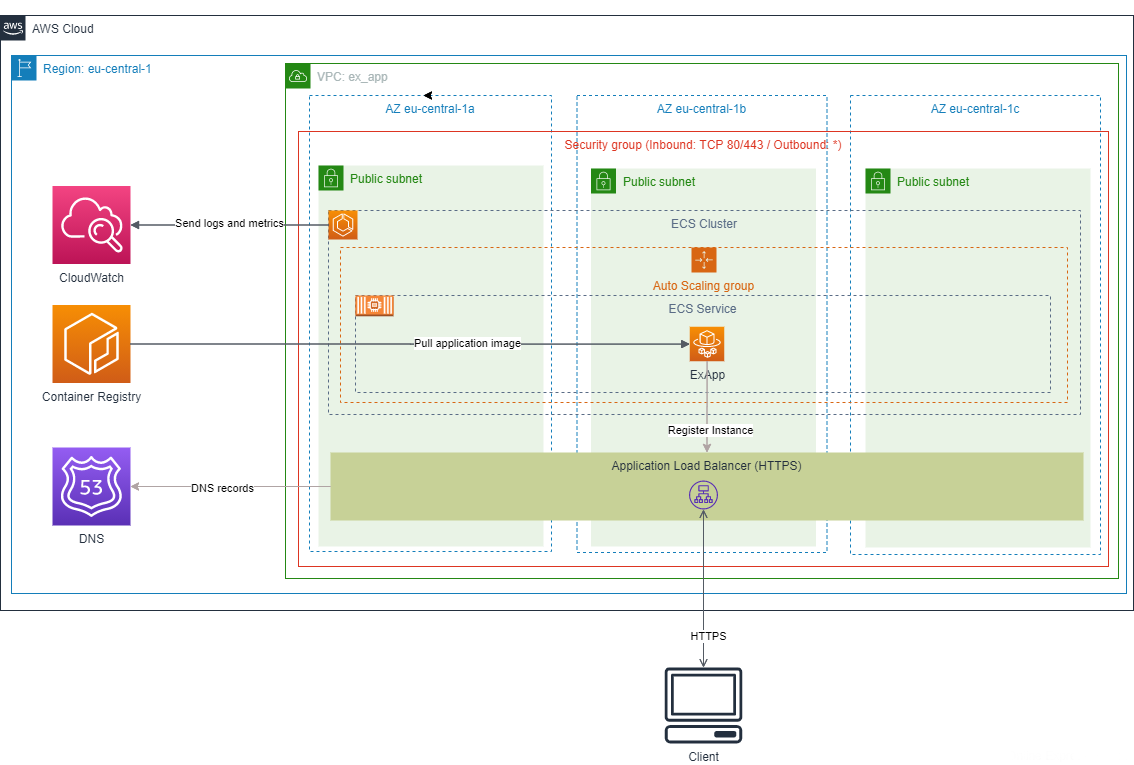
\includegraphics[width=1.0\textwidth]{images/aws_infrastruktur.png}
  \caption[AWS Infrastruktur]{AWS Infrastruktur}
  \label{fig:aws_infrastructure}
\end{figure}

\begin{itemize}
  \item Die Anwendung wird in der Region eu-central-1 (Frankfurt) installiert.
  \item Es wird eine eigene VPC mit Subnets in den drei verfügbaren AZs verwendet.
  \item Die Security Group erlaubt eingehenden Datenverkehr auf Port 80 (HTTP) und 443 (HTTPS).
  Der ausgehende Datenverkehr ist nicht beschränkt.
  \item Ein ECS Cluster der Instanzen in allen 3 Regionen starten kann wird für den ExApp Service verwendet.
  \item Der Cluster sendet Log-Ausgaben und Metriken (wie RAM/CPU Auslastung) an AWS CloudWatch.
  \item Die Images für die Tasks in dem ECS-Service werden aus der AWS Container Registry heruntergeladen.
  \item Wird ein Task gestartet, registriert er sich am Application Load-Balancer.
  Sobald der Healthcheck des Load-Balancers meldet, dass dieser auf HTTP-Anfragen antwortet, erhält der Task Traffic vom ALB.
  \item Der AWS Application Load-Balancer wird mit einem A- und AAAA-Record in Amazons Route 53 DNS registriert.
  \item Der Load-Balancer ist über HTTPS erreichbar und terminiert SSL, um die Anfragen an die jeweiligen Container weiterzuleiten.
  Clients rufen die URL vom Load-Balancer auf.
  \item Mittels AWS Metriken wird ermittelt, ob Tasks eine CPU Auslastung von > 50\% über einen Zeitraum von 60 Sekunden haben.
  Ist das der Fall werden bis zu 4 weitere Container gestartet, um die Last zu verteilen.
\end{itemize}

Die jeweiligen Terraform Skripte können beliebig unterteilt werden, die kompletten Skripte finden sich im Anhang dieser Arbeit.
Eine gängige Konvention bei der Benennung von Terraform Skripte ist diese einfach mit einer Nummer zu versehen.
Auch wenn Terraform die Reihenfolge bei der Erstellung der Ressourcen selbst ermittelt, so ist es doch hilfreich die Reihenfolge und Art der Ressourcen auf diese Art und Weise zu gruppieren.

\paragraph{VPC}

Jede Installation der Anwendung läuft in einer separate \hyperref[lst:terraform_vpc]{VPC} mit einem eigenen Internet Gateway und einer Route Table.
Der CIDR der VPC ist immer 172.16.1.0/24.
Die jeweiligen Subnetze sind über mehrere AZs verteilt und unterstützen bis zu 254 Adressen.

In der Region Frankfurt (eu-central-1) können somit insgesamt 762 Container über alle drei Subnetze verteilt verwendet werden.

\paragraph{Security Groups}

Mit \hyperref[lst:terraform_security_group]{Security Groups} werden die Firewall Regeln für eine \hyperref[lst:terraform_vpc]{VPC} und ihre Subnetze dargestellt.
Die Anwendung erlaubt hierfür eingehenden Datenverkehr auf Port 80 HTTP und 443 HTTPS.
Ausgehender Datenverkehr und Datenverkehr innerhalb der VPC ist ebenfalls erlaubt.

\paragraph{ECS}

Für die Anwendung wird AWS Elastic Container Service ECS verwendet.
Dafür muss ein entsprechender \hyperref[lst:terraform_ecs]{ECS Cluster} definiert werden.
Diesem Cluster sind keine Server zugeordnet und er verursacht dadurch keine zusätzlichen Kosten.

Für AWS Fargate wird hier noch zusätzlich eine \hyperref[lst:terraform_fargate_role_policy]{IAM Policy} definiert.
Diese erlaubt den Zugriff auf ECR für die Docker Images und CloudWatch für die Logs.


\paragraph{Task und Service}

ECS unterscheidet zwischen Tasks und Services.
Ein Service besteht aus einem oder mehreren Tasks der gleichen Task-Definition.
Für die Task-Definition wird eine \hyperref[lst:terraform_ecs_task_json]{JSON Datei} erstellt, dort werden die Docker Einstellungen des Containers vorgenommen.

Es lassen sich auch mehrere Container innerhalb einer Task-Definition starten und konfigurieren.
Wird ein als \textbf{Essential} markierter Container beendet, so wird der gesamte Task von AWS neu gestartet.

Aus einer Task-Definition wird ein \hyperref[lst:terraform_ecs_task]{Task} erstellt.
Dieser wird dann in einem Service gestartet.
Bei der Definition des Services wird auch angegeben, wie viele Instanzen von einem Task in einem Service gestartet werden sollen.


\paragraph{Autoscaling}

Mit \hyperref[lst:terraform_autoscaling]{Autoscaling} kann man automatisch mehrere Tasks starten lassen, wenn bestimmte Bedingungen erfüllt sind.
Die aktuelle Konfiguration überwacht die CPU Auslastung, liegt diese über einen Zeitraum von 60 Sekunden bei mehr als 50\%, wird ein zusätzlicher Task innerhalb des Services gestartet.
Dabei werden maximal 4 Instanzen eines Tasks gestartet.
Fällt die CPU Last unter 50\% werden die Tasks automatisch entfernt.
Es lassen sich beliebige Metriken aus AWS CloudWatch verwenden.
Auf diese Art und Weise kann man eine Anwendung automatisch skalieren.

\paragraph{Application Load-Balancer}

Die Anwendung verwendet einen \hyperref[lst:terraform_alb]{AWS Load-Balancer}.
Hierfür wird der Application-Load-Balancer für HTTP und HTTPS verwendet.

Der ALB verwendet Target-Groups, um die ECS Fargate-Tasks anzusprechen.
Hier befindet sich auch ein Health-Check der periodisch eine Anfrage an die Tasks sendet.
Werden diese Anfragen mit einem HTTP Status Code kleiner als 500 beantwortet, so wird dieser Task weiterhin Traffic von dem Load-Balancer erhalten.

Der ALB hat zwei Listener.
Einen für HTTP der die Anfragen auf HTTPS umleitet und den HTTPS Listener.
Der HTTPS Listener verwendet ein Wildcard Zertifikat von AWS (*.kuffel.me) und terminiert den SSL Verkehr in Richtung der Tasks.

Der ALB regelt die Verteilung des Traffics und die Tasks melden sich an dem ALB an und ab.
Wenn ein ECS Task beendet wird, hört der ALB auf diesem weitere Anfragen zu senden.

Bei einem Update der Container bleibt die Anwendung jederzeit verfügbar.
Alte Container bekommen so lange Anfragen bis die neuen Container am ALB registriert sind.
Anschließend werden diese am ALB abgemeldet und von ECS beendet.

\paragraph{DNS}

Der ALB hat einen CNAME im AWS eigenen DNS Route 53, an dem Load-Balancer hängt ein Wildcard Zertifikat, dieses würde mit dem ALB CNAME von keinem Browser akzeptiert.
Über Route 53 wird ein \hyperref[lst:terraform_dns]{Alias für den CNAME} des ALB eingetragen.
Dazu wird ein A-Record für IPv4 und ein AAAA-Record für IPv6 verwendet.
Um Route 53 verwenden zu können empfiehlt es sich ein eigene Hosted Zone mit einer eigenen Domain anzulegen.
Diese kann über die AWS Route 53 Konsole reserviert werden.

\paragraph{Sonstige Dateien}

Alle Ausgaben der Container werden nach AWS CloudWatch umgeleitet.
Dafür benötigt man eine \hyperref[lst:terraform_monitoring]{AWS Log Group}.
Diese wird ebenfalls über Terraform erstellt.
Über Cloud Watch Filter Metrics können Alarme erstellt werden, die beim Auftreten bestimmter Texte in den Logs zu einer Benachrichtigung führen.
Logs werden nach 30 Tagen automatisch wieder gelöscht.

Alle Terraform Dateien verwenden Variablen und Workspaces, um die jeweiligen Installationen voneinander zu trennen.
Die verwendeten Variablen und ihre Standardwerte werden in der \hyperref[lst:terraform_variables]{variables.tf} definiert.
Nur Variablen, die in der variables.tf definiert sind, können überschrieben werden.

Nach der Ausführung von Terraform werden neue Ressourcen angelegt.
Die Namen dieser Ressourcen sind nicht immer vorhersehbar.
Um eine Ausgabe der angelegten Ressourcen nach der Ausführung zu steuern, kann eine \hyperref[lst:terraform_output]{outputs.tf} verwendet werden.

\newpage
\subsection{Circle CI}\label{implementierung_circle_ci}

Dieser Abschnitt beschreibt die Einrichtung und Konfiguration der Circle CI-Pipeline.
Die Pipeline wird bei jedem Pull Request auf GitHub gestartet.
Bei jedem akzeptierten Pull Request für den Master wird die gleiche Pipeline durchgeführt.

\subsubsection{Grundlagen}

Circle CI verwendet für die Beispiele vereinfachte Konfigurationen.
Für komplexere Abläufe lassen sich Konfigurationen für die Version 2.1. erstellen.
Diese haben folgende Unterteilung und erlauben die Wiederverwendung von einzelnen Schritten.
\footnote{{Orbs, Jobs, Steps, and Workflows, vgl.~\cite{CIRCLE_ORBS_JOBS_STEPS_WORKFLOWS}}}

\begin{itemize}
  \item \textbf{Executors:}
  Durch Executors lässt sich die Ausführungsumgebung in Circle CI bestimmen.
  Dabei können verschiedene Executors für unterschiedliche Schritte verwenden werden.
  Der Docker Executor startet das gewünschte Docker Image und führt alle Schritte innerhalb dieses Containers durch.
  Ein Machine Executor kann Linux, Windows oder MacOS verwenden und führt die Schritte direkt auf einer VM durch.
  \footnote{{Executors and Images, vgl.~\cite{CIRCLE_EXECUTORS_INTRO}}}

  \item \textbf{Commands:}
  Mit Commands lassen sich Abfolgen von Schritten für die Wiederverwendung gruppieren.
  Ein Command wird benannt und lässt sich in den Jobs immer wieder aufrufen.

  \item \textbf{Jobs:}
  Jobs sind benannte Abfolgen von eingebauten Commands und selbst definierten Commands.
  Hierbei wird auch der Executor festgelegt, d.h. die Umgebung in der ein Job ausgeführt werden soll.

  \item \textbf{Workflows:}
  Definiert eine Abfolge von Jobs.
  Hierbei können Bedingungen, wie der aktuelle Branch, definiert werden.

  \item \textbf{Orbs:}
  Bei Orbs handelt es sich um wiederverwendbare Konfiguration für Commands, Jobs und Workflows.
  In einer CI-Pipeline muss immer wieder Software auf den Executors installiert und konfiguriert werden.
  Die AWS CLI erfordert z.B. die Installation von Python und die Konfiguration von AWS Credentials.
  Wenn mehrere Schritte mit unterschiedlichen Executors die CLI brauchen entsteht Redundanz.
  Orbs verwenden Environment Variablen und erlauben so eine einfache Konfiguration von Jobs, die Abhängigkeiten zu Software wie z.B. AWS CLI und Terraform haben.
\end{itemize}

\subsubsection{Einrichtung}

Um Circle CI zu verwenden muss zunächst ein kostenloser Account angelegt werden.
Dafür kann man sich direkt mit seinem GitHub Account registrieren.
Nachdem man Circle CI die entsprechenden Berechtigungen im Github Account eingeräumt hat, erscheint eine Liste aller Projekte, die im eigenen GitHub Account verfügbar sind.

Wenn man ein Projekt mit \textbf{Set Up Project} auswählt, kann direkt ein neuer Commit mit der Circle CI Konfiguration erstellt werden.
Über ein Dropdown kann hier eine vorgefertigte Konfiguration für die verwendete Programmiersprache ausgewählt werden.

Nachdem man die Änderungen mit \textbf{Commit and Run} bestätigt, erzeugt Circle CI einen Commit und eine erste Pipeline wird gestartet.

\paragraph{Executors und Orbs}

Die Pipeline für die Beispielanwendung verwendet zwei Arten von Executors:

\begin{itemize}
  \item \textbf{Docker Executor:}
  Verwendet ein Elixir Docker Image für die Schritte, die eine Elixir Umgebung benötigen.

  \item \textbf{Machine Executor:}
  CircleCI Linux Maschine für Terraform, Docker und AWS CLI Operationen.
\end{itemize}

Die Beispielanwendung benötigt die AWS CLI, um Images in AWS ECR veröffentlichen zu können.
Dafür gibt es zwei offizielle Orbs von CircleCI:

\begin{itemize}
  \item \textbf{AWS CLI}
  Dieser Orb installiert und konfiguriert die AWS CLI in einem Machine Executor.
  Die Konfiguration der AWS Access Keys erfolgt dabei über die Umgebungsvariablen, die über die CircleCI Benutzeroberfläche konfiguriert werden.
  Dieser Orb kann einfach mit \texttt{aws-cli/setup} in den Steps verwendet werden.
  In den darauffolgenden Schritten steht dann die AWS CLI zur Verfügung.
  \footnote{{Orbs AWS CLI, vgl.~\cite{CIRCLE_ORBS_AWS_CLI}}}

  \item \textbf{AWS ECR}
  Um Images in AWS ECR publizieren zu können, muss der Docker Client sich an der Registry anmelden.
  Dieser Orb ermöglicht den Docker Login an ECR mit dem Schritt \texttt{aws-ecr/ecr-login}
  \footnote{{Orbs AWS ECR, vgl.~\cite{CIRCLE_ORBS_AWS_ECR}}}
\end{itemize}

Die Circle CI Konfiguration wird unter \hyperref[lst:circle_orbs_and_executors]{.circleci/config.yml} abgelegt.

\subsubsection{Commands}

Für die Pipeline wurden sich ständig wiederholende Schritte als Commands definiert.
Diese werden dann in den jeweiligen Jobs wiederverwendet.

\begin{itemize}
  \item \textbf{setup\_elixir:}
  Dieses Kommando richtet zunächst die Elixir und Erlang Paketmanager Hex und Rebar ein.
  Die Abhängigkeiten werden kompiliert und zusammen mit einer Prüfsumme über die Datei mix.lock im Cache abgelegt.
  Falls die Abhängigkeiten bereits kompiliert wurden, können sie bei einer Wiederholung dieses Kommandos aus dem Cache geladen werden.
  Das vollständige Kommando findet sich im Anhang unter \hyperref[lst:circle_command_setup_elixir]{Circle CI - Command - setup\_elixir}.

  \item \textbf{setup\_terraform:}
  Terraform wird für das Deployment verwendet.
  Die CLI wird verwendet, um Terraform Dateien zu validieren, Umgebungen zu löschen und zu erstellen.
  Dieses Kommando lädt die CLI herunter und kopiert diese in das entsprechende Linux Verzeichnis.
  Das vollständige Kommando befindet sich im Anhang unter \hyperref[lst:circle_command_setup_terraform]{Circle CI - Command - setup\_terraform}.

\end{itemize}

\subsubsection{Jobs}

Jobs sind eine Abfolge von Kommandos, die später in einem Workflow eingesetzt werden.
Jeder Job definiert somit die Schritte und den Executor auf dem dieser ausgeführt werden soll.
Dabei ist zu beachten, dass Jobs immer mit einem neuen Executor gestartet werden.
Das erlaubt die Parallelisierung.
Es erfordert jedoch auch immer die Initialisierung der Umgebung.

\paragraph{Statische Codeanalyse}

Dieser \hyperref[lst:circle_job_check_code]{Schritt} überprüft die Formatierung mit \texttt{mix format} und den Code statisch nach den Regeln von Credo mit der Ausführung von \texttt{mix credo}.
Schlägt einer dieser beiden Schritte fehl, wird die gesamte CI/CD Pipeline als fehlgeschlagen markiert.
Der Ersteller des Pull Requests erhält ein frühes Feedback darüber, dass der Code nicht korrekt formatiert ist oder nicht den festgelegten Regeln enspricht.

\paragraph{Kompilierung}

In diesem \hyperref[lst:circle_job_build]{Schritt} werden die Quellen des Projekts kompiliert.
Dabei wird das Kommando \texttt{mix compile --force --warnings-as-errors} verwendet.
Wenn Warnungen bei der Kompilierung auftreten, wird die CI/CD Pipeline als fehlgeschlagen markiert.
Der Parameter \texttt{--warnings-as-errors} soll dazu dienen, nicht verwendete Variablen früh im Buildprozess zu erkennen und den Entwickler darauf hinzuweisen.

\paragraph{Tests}

Bei diesem \hyperref[lst:circle_job_test]{Schritt} werden die Unit Tests der Anwendung mit \texttt{mix test} ausgeführt.
Wenn Tests fehlschlagen wird die gesamte Pipeline als fehlgeschlagen markiert und beendet.
Die Tests verwenden coverall, um zu ermitteln welche Testabdeckung erreicht wurde.
Wird die gewünschte Abdeckung nicht erreicht, so wird die Pipeline als Fehlschlag beendet.

\paragraph{Dokumentation}

Bei diesem \hyperref[lst:circle_job_documentation]{Schritt} wird die Dokumentation mit \texttt{mix test} erstellt.
Die erstellte ZIP-Datei wird im Anschluss unter den Build Artefakten in Circle CI abgelegt.
Die Dokumentation kann nach einem Build über die Oberfläche von Circle CI heruntergeladen werden.

\paragraph{Docker}

Zur Erstellung der Docker Container wird zunächst die Versionsnummer in der Anwendung aktualisiert.
Dazu wird ein \hyperref[lst:projekt_version_sh]{Skript} aufgerufen, das die aktuelle Semantic Version mit dem Git Commit Hash ergänzt.
Anschließend wird das Docker Image durch Aufruf von \texttt{make docker} erstellt.

Dieses Image muss getaggt und in AWS ECR veröffentlicht werden.
Dazu wird der AWS CLI und AWS ECR Orb verwendet.
Als Docker Tag wird hier ebenfalls die Version und der Git Commit Hash verwendet.
Da Docker Tags kein Pluszeichen zur Trennung von Version und Hash unterstützen, muss mit einem Bindestrich getrennt werden. \\

Abschließend wird das Image in das AWS ECR Repository gepusht und steht somit für ein Deployment zur Verfügung.
Die YAML Definition des \hyperref[lst:circle_job_docker]{Schritts} befindet sich im Anhang.

\paragraph{AWS Lambda Funktion}

Nicht alle Teile der CI-Pipeline lassen sich einfach in Orbs oder Shell Skripten implementieren.
Gerade Schritte die REST-APIs von AWS und GitHub verwenden ist der Einsatz von Python empfehlenswert. \\

Es wurde AWS Chalice verwendet.
Es handelt sich dabei um ein Python Framework mit dem serverlose AWS Lambda Funktionen erstellt werden können. \footnote{{AWS Chalice, vgl.~\cite{AWS_CHALICE}}}
Diese Funktionen lassen sich über eine REST API verwenden.
Somit wird vermieden in der CI-Pipeline Python Skript auszuführen. \\

Diese \hyperref[lst:lambda_app_py]{REST Endpunkte} wurden dafür implementiert:

\begin{itemize}
  \item \texttt{POST /cleanup\_images:}
  Verwendet die Python AWS-Library, um zu ermitteln welche ECR Images gerade noch in einem ECS-Cluster verwendet werden.
  Nicht verwendete Images werden automatisch gelöscht.
  Dieses Vorgehen spart Kosten für die Speicherung von nicht verwendeten Images in ECR.

  \item \texttt{GET /pull-requests:}
  Gibt eine Liste aller Pull Requests in dem ex\_app Github Projekt zurück.

  \item \texttt{GET /unused-workspaces:}
  Ermittelt anhand bereits geschlossener Pull Requests und der Terraform Statefiles im S3 Bucket welche Deployments nicht mehr benötigt werden.
  Diese Deployments und Workspaces können im Rahmen eines Master Build Workflows entfernt werden.

  \item \texttt{POST /add-comment/{PULL\_REQUEST\_ID}:}
  Erzeugt einen neuen Kommentar in dem GitHub Pull Request.
  Dieser Endpunkt wird dazu verwendet, den Kommentar mit der URL zu der Vorschauumgebung zu erzeugen.
\end{itemize}

Die jeweiligen Endpunkte werden mit Bash Skripten aus der CI/CD Pipeline heraus aufgerufen.
Diese Bash Skripte können einfach mit dem in Linux integrierten Kommando \texttt{wget} implementiert werden.

\paragraph{Vorschauumgebung installieren}

Damit der Reviewer des Pull Requests neben den Code-Änderungen die Änderungen auch direkt in der Anwendung anschauen kann, wird eine \hyperref[lst:circle_job_deploy_preview]{Vorschauumgebung installiert}.
Dadurch werden die Terraform Skripte verifiziert und ein Reviewer muss kein eigenes Deployment durchführen. \\

In dem Job wird zunächst die AWS CLI konfiguriert, Terraform installiert und die Terraform Dateien validiert.
Um die Vorschauumgebung zu installieren, wird ein eigener Terraform Workspace erstellt.
Dieser Workspace bekommt die ID des Pull Requests mit dem Prefix \texttt{preview\_}. \\

Danach wird die Infrastruktur mit \texttt{terraform apply} und unter Verwendung der entsprechenden Variablen installiert.
Nachdem \texttt{terraform apply} durchgeführt wurde, kann es einige Minuten dauern bis das Deployment tatsächlich bereitsteht. \\

Um zu erkennen ob die gewünschte Version der Anwendung installiert ist wurden zwei zusätzliche HTTP Response Header eingefügt.
Diese enthalten in einem \texttt{x-app-version} Header die Versionsnummer und in einem \texttt{x-app-build} Header den Git Commit Hash in jeder HTTP-Antwort. \\

Das Skript \hyperref[lst:scripts_wait_for_deployment]{\texttt{wait\_for\_deployment.sh}} bekommt die geplante URL zur Vorschauanwendung und den erwartetet Git Commit Hash als Parameter.
Damit ruft das Skript periodisch die URL auf und prüft, ob eine Antwort mit dem erwarteten Header zurückkommt.
Zwischen den Versuchen wartet das Skript 10 Sekunden und nach maximal 10 Minuten wird das Deployment als fehlgeschlagen markiert.

Wenn der Header erfolgreich erkannt wurde, wird über die AWS Lambda Funktion und das Skript \hyperref[lst:scripts_add_pr_comment]{\texttt{add\_pr\_comment.sh}}
ein GitHub Kommentar mit der Vorschau URL in dem Pull Request erstellt.

\paragraph{Vorschauumgebungen entfernen}

Nachdem eine Vorschauumgebung installiert worden ist, unterscheidet sich diese für AWS nicht von einem regulären Deployment.
Diese Umgebung würde also dauerhaft bestehen bleiben und so Kosten erzeugen.
Nachdem der Pull Request akzeptiert oder geschlossen wurde, kann die Umgebung entfernt werden. \\

Dieser \hyperref[lst:circle_job_remove_preview_deployments]{Schritt} in der Circle CI-Pipeline soll das sicherstellen
und verwendet dafür die Lambda Funktion.
Es soll ermittelt werden welche Workspaces gelöscht werden können.
Dazu werden die Terraform Workspaces ermittelt bei denen kein offener Pull Request mehr vorliegt.
Diese Workspaces werden folglich nicht mehr benötigt und werden in diesem Schritt automatisch entfernt.

\paragraph{Installation in Produktivumgebung}

In diesem \hyperref[lst:circle_job_deploy_production]{Schritt} wird die Anwendung in der Produktivumgebung ausgerollt.
Nach jedem angenommenen Pull Request oder einer Änderung auf dem Master Branch wird die Produktivumgebung aktualisiert.
Dafür wird der \texttt{production} Workspace in Terraform verwendet um die Images die im Rahmen der Pipeline für den Master Branch entstehen zu installieren. \\

Das Installieren der Anwendung im Produktivsystem unterscheidet sich nur geringfügig von der Installation einer Vorschauumgebung.
Der Circle CI Job verwendet die gleichen Schritte mit abgeänderten Parametern für das Deployment. \\

Nachdem der Master erfolgreich deployed wurde, werden durch einen Aufruf an die AWS Lambda Funktion nicht mehr verwendete ECR Images gelöscht.

\subsubsection{Workflow}

Die zuvor implementierten Schritte werden in einem Workflow in Circle CI abgebildet.
Mit Workflows lässt sich festlegen, welche Jobs in welcher Reihenfolge und unter welchen Bedingungen ausgeführt werden sollen. \\

Grundsätzlich würde Circle CI die Jobs parallel ausführen.
Durch die Angabe der Abhängigkeiten mit dem Schlüsselwort \texttt{requires} kann eine Reihenfolge definiert werden.
Jeder Job unterstützt zusätzlich die Angabe eines Filters.
Damit kann gesteuert werden, ob ein Job nur auf einem bestimmten Branch durchgeführt werden soll.

\begin{itemize}
  \item \textbf{Statische Codeanalyse:}
  Dieser Schritt wird immer als erstes und auf allen Branches ausgeführt.

  \item \textbf{Kompilierung:}
  Dieser Schritt wird immer nach der statischen Codeanalyse ausgeführt.

  \item \textbf{Tests:}
  Nachdem die Kompilierung erfolgreich war, werden die Tests gestartet.

  \item \textbf{Dokumentation:}
  Die Erstellung der Dokumentation startet parallel, nachdem die Kompilierung und die Tests erfolgreich waren.

  \item \textbf{Docker:}
  Nach erfolgreichen Tests wird eine Docker Image generiert und in ECR veröffentlicht.

  \item \textbf{Vorschauumgebung installieren:}
  Dieser Schritt wird nur durchgeführt, wenn der Workflow nicht auf dem Master Branch durchgeführt wird.

  \item \textbf{Vorschauumgebungen entfernen:}
  Entfernt die Vorschauumgebungen, wenn der Master-Branch im aktuellen Workflow gebaut wird.

  \item \textbf{Installation in Produktivumgebung:}
  Wird nur auf dem Master Branch durchgeführt und nimmt das Deployment in die Produktivumgebung vor.
\end{itemize}

Auch nach einem akzeptierten Pull Request werden die Schritte, die für einen Pull Request bereits durchgeführt wurden erneut durchgeführt.
Das soll sicherstellen, dass der Master-Branch die gleichen Tests durchläuft und sich ein Deployment für die Vorschauumbgebung kaum von einem Produktivdeployment unterscheidet.
Bei einem nicht akzeptierten Pull Request wird die Vorschauumgebung spätestens beim nächsten Master-Branch Build entfernt. \\

Der komplette Ablauf ist im Anhang unter \hyperref[lst:circle_workflows]{Circle CI - Workflows} definiert.


\newpage
\subsection{Zusammenfassung}\label{implementierung_zusammenfassung}

Der vollständige Workflow der CI/CD Pipeline wird im untenstehenden Bild dargestellt.

\begin{figure}[htb]
    \centering
    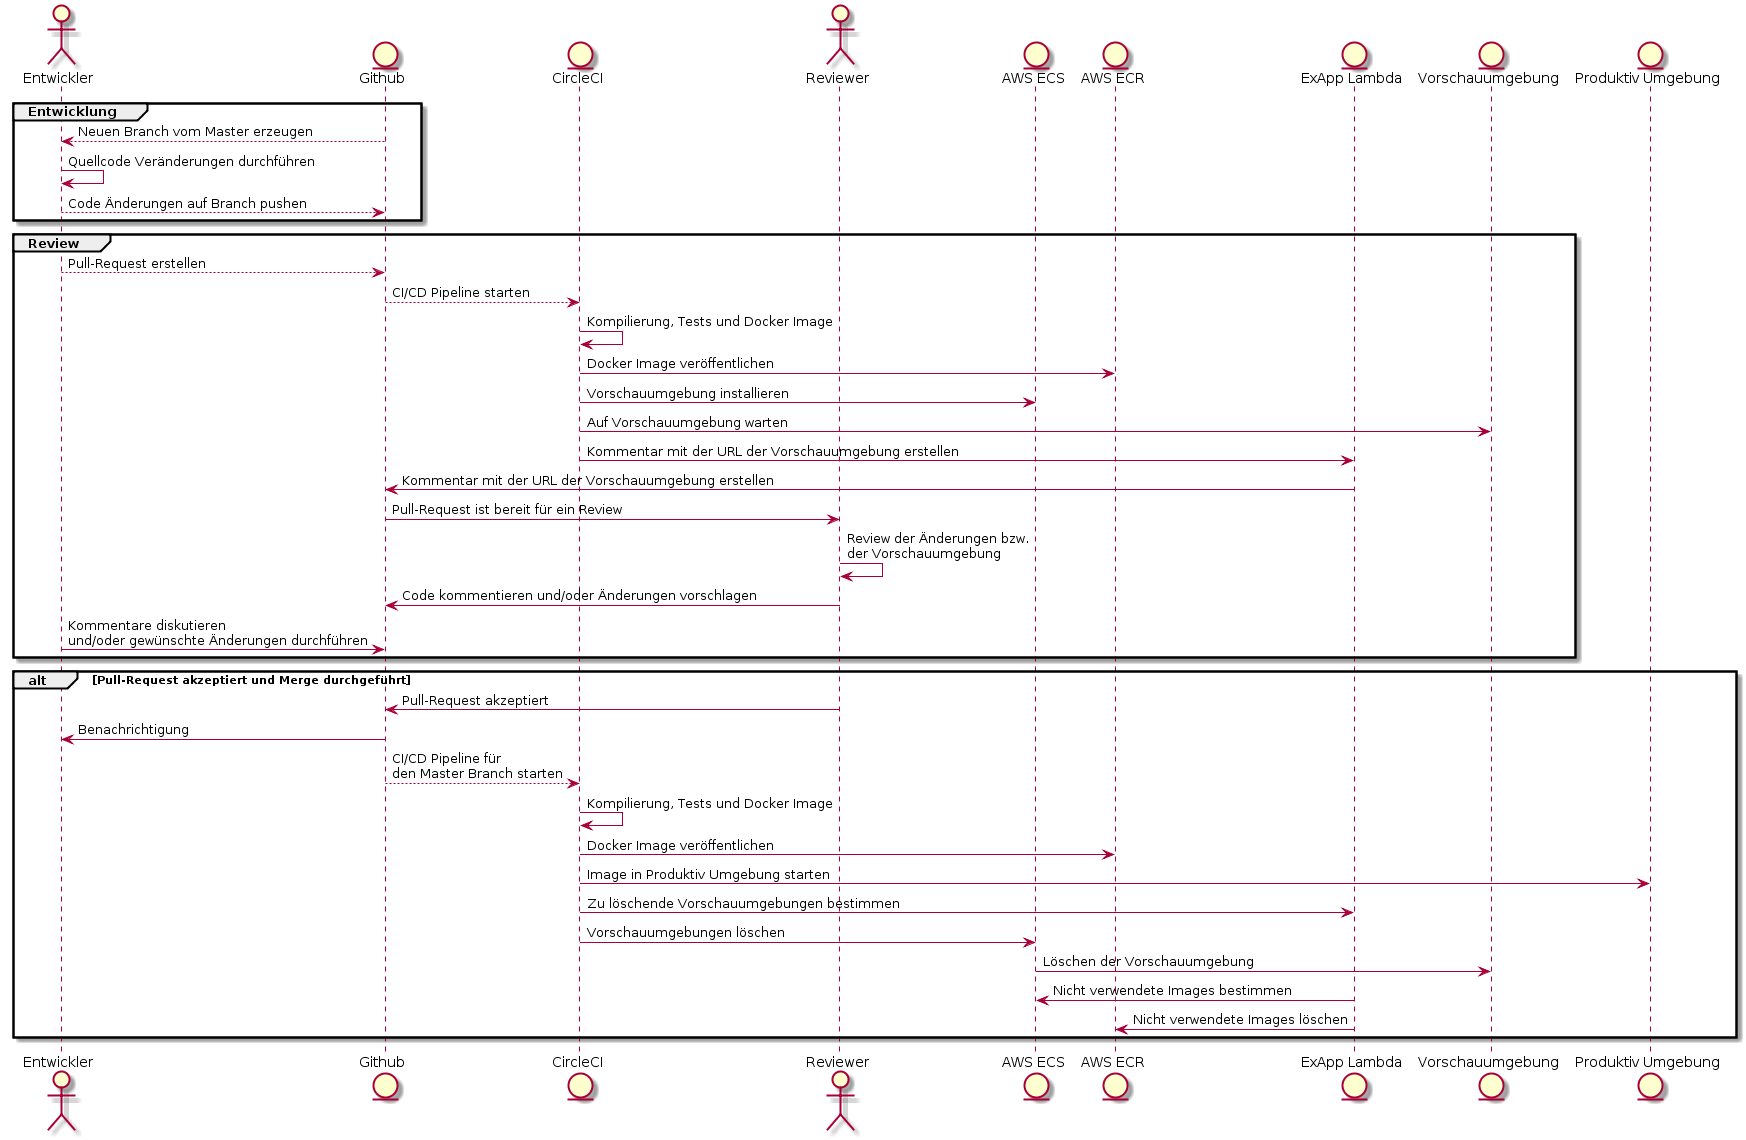
\includegraphics[width=1.0\textwidth]{images/workflow.png}
    \caption[Circle CI Workflow]{Circle CI Workflow}
    \label{fig:circle_ci_workflow}
\end{figure}

Die implementiere CI/CD-Pipeline ermöglicht eine Self Service Infrastruktur.
Entwickler können durch Veränderungen an den Terraform Skripten die Infrastruktur anpassen.
Die Pipeline führt diese Änderungen aus und ermöglicht durch das Bereitstellen einer Vorschauumgebung effiziente Review Prozesse. \\

Der Entwickler muss nur einen Pull Request öffnen, um die Automatisierung zu starten.
Nach Abschluss aller Tests und der testweisen Veröffentlichung kann ein Review durchgeführt werden.
Der Reviewer kann die Veränderungen direkt in der Vorschauumgebung ausprobieren. \\

Wird ein Pull-Request akzeptiert, genügt ein Knopfdruck um den Pull-Request zu akzeptieren und damit den neuen Code in die Produktion zu überführen.
Im Fehlerfall kann eine Änderung in Git wieder rückgängig gemacht werden und die CI/CD Pipeline wird die vorherige Version wiederherstellen.



\newpage

% Fazit
\fancyhead[L]{\nouppercase{Fazit}}
\section{Fazit}\label{fazit}

Eine Umsetzung einer DevOps Strategie ist bei Neuentwicklungen einfacher, da es nicht notwendig ist eingefahrene Abläufe zu ändern.
Die technischen Voraussetzungen lassen sich bei neuen Projekten ebenfalls von Anfang an berücksichtigen.
Eine nachträgliche DevOps Migration lässt sich mit den beschriebenen Wegen jedoch schrittweise ebenfalls durchführen. \\

Die Verwendung von agilen Methoden und DevOps erlaubt es, dass Unternehmen kleine Iterationen durchzuführen, kontinuierliches Feedback und eine schnelle Reaktion auf geänderte Anforderungen.
Ein Einsatz von agilen Methoden ohne kontinuierliches Deployment der Änderungen macht kaum Sinn, da DevOps ein Enabler für agile Entwicklung ist.
DevOps und agile Methoden sollten also immer gemeinsam verwendet werden. \\

Bei der Betrachtung der Kollaborationstools fällt auf, dass sich Git als Versionskontrolle durchgesetzt hat.
Andere Systeme werden kaum verwendet.
Die Anbieter von Webbasierten Tools wie GitLab, GitHub und BitBucket bieten alle einen ähnlichen Funktionsumfang.
GitLab tritt dabei als Lösung hervor, in der alles in einem Tool erledigt werden kann.
Neben der Versionskontrolle ist dort ein Ticketsystem, CI/CD Pipelines und Tools fürs Projektmanagement sowie Sicherheit/Compliance vorhanden. \\

Bei den CI/CD Serverlösungen wird oft Jenkins verwendet.
Dafür ist es jedoch notwendig diesen auf eigenen Servern zu installieren.
Mit über 1.500 Plugins kann jedes Szenario mit Jenkins abgebildet werden.
Das macht die Verwaltung und insbesondere die Durchführung von Updates komplex.
Bei den cloudbasierten CI/CD Systemen kommt in der Regel YAML mit einer DSL zum Einsatz.
Die Skripte sind deutlich lesbarer als die Groovy basierten Jenkinsfiles. \\

Mit Circle CI hat man eine gute Integration in GitHub.
Es lässt sich allerdings auch nur mit BitBucket und GitHub verwenden.
Besonders die Orbs und das Docker Layer Caching erlauben hier die einfache Erstellung schneller CI/CD Pipelines. \\

Für die Provisionierung von Infrastruktur in einer Public Cloud erscheint Terraform die erste Wahl zu sein.
Keines der betrachteten Tools stellt die Provisionierung von Infrastruktur an erste Stelle.
Die anderen Tools sind eher zur Verwaltung bereits vorhandener Infrastruktur geeignet.
Durch die Unterstützung von sogenannten Providern lassen sich mit Terraform auch bereits vorhandene Dienste verwalten.
Die Abgrenzung zwischen Provisionierung und Konfigurationsmanagement ist somit auch bei Terraform nicht ganz deutlich. \\

Die Dienste von AWS sind im Vergleich zu Google Cloud und Azure wesentlich umfangreicher.
Gerade im Bereich CaaS bietet AWS mit ECS eine Alternative zu Kubernetes an.
Die Einarbeitung in Kubernetes ist deutlich aufwendiger als in ECS und mit Fargate bietet Amazon die Möglichkeit Container serverlos zu betreiben.
Bei der Verwendung von ECS zahlt man ausschließlich für die Ressourcen anders als bei den meisten Kubernetes Lösungen, bei denen bereits das Dashboard kostenpflichtig ist. \\

Für die technische Umsetzung von CI/CD Pipelines gibt eine Vielzahl von Möglichkeiten.
Die in dieser Arbeit implementierte Pipeline könnte in ähnlicher Form auch mit anderen Tools umgesetzt werden.
Die vorgeschlagene Lösung lässt sich jedoch vollkommen kostenlos beginnen.
Lediglich die Kosten für die Infrastruktur auf AWS sind zu entrichten.




\subsection{Zusammenfassung}\label{zusammenfassung}

Von den zuvor vorgestellten \nameref{devops_massnahmen} für eine DevOps Migration erfüllt die Implementierung vorallem die technischen Aspekte.

Durch einen hohen Grad an Automatisierung können die Teams einfach zusammenarbeiten.
Die Implementierungen können ohne großen Aufwand für ein Reviewprozess abgegeben werden, der Reviewer kann anhand der Vorschau-Umgebung
sowie des GitHub Pull-Requests Feedback geben und die Änderungen überprüfen.
Das automatisierte Testing und die regelmäßige automatische Integration sorgt dafür,
dass Änderungen schnell und sicher durchgeführt werden können. \\

Per Knopfdruck lassen sich die Änderungen anschließend ohne Ausfall, ins Produktivsystem überführen.
Im Fehlerfall kann der Merge wieder rückgängig gemacht werden und die vorherige Version wird wiederhergestellt.
Jederzeit können Entwickler dabei auch die Infrastruktur durch Anpassungen an den Terraform Skripten verändern.
Dabei ist mit der Verwendung von ECS zwar nicht alles veränderbar, es kann jedoch ohne großen Aufwand neue Infrastruktur hinzugefügt werden.
Da jede Vorschau-Umgebung vollständig vom Produktivsystem isoliert ist, besteht auch nicht die Gefahr, dass Entwicklungsarbeit das Produktivsystem gefährdet. \\

Die Implementierung erlaubt die Entwicklung von sogenannten Cloud Native Applikationen, der Betrieb eigener Infrastruktur ist nicht erforderlich.
Es kann immer auf SaaS und PaaS Dienste der AWS Cloud Infrastruktur zugegriffen werden. \\

Auf den Stufen der \nameref{devops_reifegraden} befindet sich die Lösung damit auf Stufe 4, für Stufe 5 fehlt hier lediglich die Einbindung von Sicherheitsteams.


\subsection{Kritische Reflexion}\label{kritische_reflexion}

In dieser Arbeit wurde vor allem Software verwendet, die sich bis zu einem gewissen Grad kostenlos nutzen lässt.
Gerade im Bereich DevOps und CI/CD gibt es kommerzielle Lösungen, welche versprechen alles auf einmal anzubieten.
Der Zugriff auf diese Tools ist jedoch oft nur auf Anfrage, kostenpflichtig verfügbar oder zeitlich begrenzt verfügbar.
Aus diesem Grund wurde in dieser Arbeit der Fokus auf kostenlose SaaS Angebot wie Circle CI und GitHub gelegt. \\

Die Kriterien zur Evaluierung der einzelnen Tools wurden mithilfe der Literatur, der Produktwebsites und basierend auf eigenen Versuchen ausgewählt.
Ein systematischer Vergleich war alleine aufgrund der sehr unterschiedlichen Ansätze im Bereich Kollaborationstools schwierig. \\

Die Arbeit zeigt auch, dass die Verwendung von DevOps, ein weitaus breiteres Wissen erfordert.
Durch den Einsatz von CI/CD sind wesentlich mehr Technologien, Frameworks und Tools im Einsatz.
Um DevOps verwenden zu können,s müssen Mitarbeiter also weitere Technologien beherrschen lernen. \\

Terraform verspricht einen einfachen Multi Cloud Einsatz.
Im Laufe der Arbeit zeigte sich jedoch, dass es ohne detaillierte Kenntnisse der jeweiligen Begrifflichkeiten der verschiedenen Cloud Provider,
nicht trivial ist Terraform Skript zu entwickeln.
Eine einfache Übertragung von Skripten von einem Cloud Anbieter zu einem anderen scheidet somit aus. \\

\subsection{Ausblick}\label{ausblick}

Die implementierte CI/CD Pipeline ist in erster Linie eine Basis für weiterführende Möglichkeiten.
Folgende Themen wurden im Rahmen der Arbeit betrachtet, jedoch nicht weiterverfolgt:

\begin{itemize}
    \item \textbf{Frontend Testing:}
    Mit dem UI-Testing Frameworks, wie \href{https://www.selenium.dev/}{Selenium}, lassen sich Abläufe in einem Webbrowser fernsteuern.
    Um einen Browser in der CI/CD Pipeline ohne Oberfläche zu starten, benötigt man einen WebDriver und einen passenden Browser.
    Circle CI enthält für gängige Browser Test Frameworks \href{https://circleci.com/docs/2.0/browser-testing/}{Dokumentation und Tutorials}.
    Durch automatisierte Frontend Test kann ein Review zusätzlich beschleunigt werden,
    da der Reviewer im besten Fall nicht manuell neue Features ausprobieren muss.

    \item \textbf{IaC Linting:}
    Im Rahmen der CI/CD Pipeline werden die Terraform Skripte mit dem Kommando \texttt{terraform validate} überprüft.
    Dabei wird jedoch nur die Syntax geprüft, eine Prüfung der Parameter wird dabei nicht durchgeführt.
    Ein Fehler in diesen Parametern würde somit erst beim Deployment auffallen.
    Durch das Preview Deployment werden diese Probleme früh erkannt.
    Um diese Probleme noch früher zu erkennen, könnte mit der Anwendung \href{https://github.com/terraform-linters/tflint}{tflint} eine Prüfung der Parameter vorgenommen werden.

    \item \textbf{Vollständig Automatisierung:}
    Mit vollständiger Test-Abdeckung wäre es auch möglich, eine vollständige automatisches CI/CD-Pipeline zu erstellen.
    Der Merge Request würde regulär durchgeführt werden.
    Es würde nach Abschluss aller Tests und Prüfungen ein automatischer Merge stattfinden.
    Ohne die Kontrolle durch einen menschlichen Reviewer müssten dafür eine höhere Test-Abdeckung, sowie die Möglichkeit von automatischen Rollbacks im Fehlerfall geschaffen werden.

    \item \textbf{DevSecOps:}
    Um die Stufe 5 der DevOps Reifegrade zu erreichen ist eine Einbindung von Sicherheitsteams in die Prozesse erforderlich.
    Diese Einbindung erfolgt oft unter dem Begriff DevSecOps.
    Hierfür könnten Prüfungen bereits in die CI/CD Pipeline eingebaut werden.
    Mit den Tools \href{https://github.com/tfsec/tfsec}{tfsec} und \href{https://kics.io/}{kics} lassen sich Terraform Skripte statisch auf Sicherheitsprobleme hin überprüfen.
    Für das verwendete Phoenix Framework gibt es mit \href{https://github.com/nccgroup/sobelow}{sobelow} ein weiteres statisches Codeanalyse Tool,
    welches automatisch Prüfungen auf Sicherheitsprobleme durchführen kann.
\end{itemize}

% Circle CI Paid Plans mit Docker Layer Caching um Build Zeiten zu senken
% Eigene Metriken und Telemetrie
% A/B Testing für Features
% Automatische Lasttests via z.B. loadimpact.io
%-Serverless CI/CD mit AWS Lambda
%-AWS Cloud9 ist ein intressanter Weg (Pair Programming, No Software Install)
%-AWS CodeGuru
%-User Feedback
% IaC hat oft sehr unterschiedliche Ausprägungen
% Cloud Provider haben alle Kubernetes als Option
% AWS geht mit ECS einen eigenen Weg
% AWS soweit vorraus das Azure/Google eigene Guides für ihre Eigene Terminologie vs AWS haben
% AWS CodeStar Tools für große Unternehmen die alles auf AWS Integrieren möchten gut.


\newpage

% \input{beispiel}

% einfacher Zeilenabstand
\singlespacing
% Literaturliste soll im Inhaltsverzeichnis auftauchen
\newpage
\phantomsection
\addcontentsline{toc}{section}{Literaturverzeichnis}
% Literaturverzeichnis anzeigen
\renewcommand\refname{Literaturverzeichnis}
\bibliography{thesis}

\newpage
% das Abbildungsverzeichnis
% Verion 1: Abbildungsverzeichnis MIT führender Nummberierung endgueltig anzeigen
\listoffigures
% Abbildungsverzeichnis soll im Inhaltsverzeichnis auftauchen
\addcontentsline{toc}{section}{Abbildungsverzeichnis}

% Verion 2: Abbildungsverzeichnis OHNE führende Nummberierung endgueltig anzeigen
%\begingroup
%\renewcommand\numberline[1]{}
%\listoffigures
%\endgroup


% das Tabellenverzeichnis
\newpage
\fancyhead[L]{\nouppercase{Tabellenverzeichnis}}
% \fancyhead[L]{Abbildungsverzeichnis / Abkürzungsverzeichnis} %Kopfzeile links
% Tabellenverzeichnis endgültig anzeigen
\listoftables
% Tabellenverzeichnis soll im Inhaltsverzeichnis auftauchen
\addcontentsline{toc}{section}{Tabellenverzeichnis}

%% WORKAROUND für Listings
%\makeatletter% --> De-TeX-FAQ
%\renewcommand*{\lstlistoflistings}{%
%  \begingroup
%    \if@twocolumn
%      \@restonecoltrue\onecolumn
%    \else
%      \@restonecolfalse
%    \fi
%    \lol@heading
%    \setlength{\parskip}{\z@}%
%    \setlength{\parindent}{\z@}%
%    \setlength{\parfillskip}{\z@ \@plus 1fil}%
%    \@starttoc{lol}%
%    \if@restonecol\twocolumn\fi
%  \endgroup
%}
%\makeatother% --> \makeatletter
% das Listingverzeichnis
\newpage
\fancyhead[L]{Listingverzeichnis} %Kopfzeile links
\renewcommand{\lstlistlistingname}{Listingverzeichnis}
\lstlistoflistings
% Listingverzeichnis soll im Inhaltsverzeichnis auftauchen
\addcontentsline{toc}{section}{Listingverzeichnis}
%%%%

% das Abkürzungsverzeichnis
\newpage
% das Abkürzungsverzeichnis ausgeben
\fancyhead[L]{Abkürzungsverzeichnis} %Kopfzeile links
\nomenclature{ACS}{Azure Container Service}
\nomenclature{AD}{Active Directory}
\nomenclature{AZ}{Availiblity Zone}
\nomenclature{ALB}{Application Load Balancer}
\nomenclature{API}{Application Programming Interface}
\nomenclature{AWS}{Amazon Webservices}
\nomenclature{CAMS}{Culture, Automation, Measurement, Sharing}
\nomenclature{CaaS}{Container-as-a-Service}
\nomenclature{CD}{Continuous Deployment/Delivery}
\nomenclature{CI}{Continuous Integration}
\nomenclature{CLI}{Command Line Interface}
\nomenclature{DNS}{Domain Name System}
\nomenclature{DSL}{Domain Specific Language}
\nomenclature{ECS}{EC2 Container Service}
\nomenclature{EKS}{Elastic Kubernetes Service}
\nomenclature{EOL}{End of Life}
\nomenclature{GCP}{Google Cloud Platform}
\nomenclature{GKE}{Google Kubernetes Service}
\nomenclature{GPU}{Graphics processing unit}
\nomenclature{HTTP}{Hypertext Transfer Protocol}
\nomenclature{JSON}{JavaScript Object Notation}
\nomenclature{IaC}{Infrastructure-as-Code}
\nomenclature{IAM}{Identity and Access Management}
\nomenclature{IaaS}{Infrastructure-as-a-Service}
\nomenclature{IDE}{Integrated Development Environment}
\nomenclature{LDAP}{Lightweight Directory Access Protocol}
\nomenclature{MVP}{Minimum Viable Product}
\nomenclature{PaaS}{Platform-as-a-Service}
\nomenclature{REST}{Representational state transfer}
\nomenclature{S3}{Simple Storage Service}
\nomenclature{SaaS}{Software-as-a-Service}
\nomenclature{SCM}{Source Code Management}
\nomenclature{TCP}{Transmission Control Protocol}
\nomenclature{UDP}{User Datagram Protocol}
\nomenclature{VCS}{Version Control System}
\nomenclature{VoIP}{Voice over IP}
\nomenclature{YAML}{Yet another markup language}



\printnomenclature[3cm]
% Abkürzungsverzeichnis soll im Inhaltsverzeichnis auftauchen
\addcontentsline{toc}{section}{Abkürzungsverzeichnis}


%% Index soll Stichwortverzeichnis heissen
% \newpage
% % Stichwortverzeichnis soll im Inhaltsverzeichnis auftauchen
% \addcontentsline{toc}{section}{Stichwortverzeichnis}
% \renewcommand{\indexname}{Stichwortverzeichnis}
% % Stichwortverzeichnis endgültig anzeigen
% \printindex

\onehalfspacing
% evtl. Anhang
\newpage
\phantomsection
\addcontentsline{toc}{section}{Anhang}
\fancyhead[L]{Anhang} %Kopfzeile links
\subsection*{Anhang}\label{anhang}

\subsubsection*{GitHub Repository}\label{anhang_github}

Der gesamte ausführbare Quellcode steht auch auf Github zur Verfügung: \\

\href{https://github.com/kuffel/ex\_app}{https://github.com/kuffel/ex\_app} \\

Zur Abgabe wurde ein Git Tag (\textbf{abgabe}) mit folgendem Git Commit Hash erstellt: \\

%%%%%%%%%%%%%%%%%%%%%%%%%%%%%%%%%%%%%%%%%%%%%%%%%%%%%%%%%%%%%%%%%%%%
\texttt{HIER\_COMMIT\_HASH\_EINFÜGEN}
%%%%%%%%%%%%%%%%%%%%%%%%%%%%%%%%%%%%%%%%%%%%%%%%%%%%%%%%%%%%%%%%%%%%
\\

Ein Pull-Request in dem Projekt wird die in der Arbeit erstellte CI/CD Pipeline starten. \\

Die LaTex Dateien zu der Thesis befinden sich im Verzeichnis \textbf{thesis}.

\subsubsection*{Quellen}\label{anhang_quellen}

Die flüchtigen Quellen der Arbeit wurden zusammen mit der Arbeit hochgeladen.
Eine ZIP Datei mit den Quellen lässt sich zusätzlich auch hier herunterladen: \\

\href{https://www.kuffel.eu/thesis/quellen.zip}{https://www.kuffel.eu/thesis/quellen.zip} \\

Die Prüfsummen der Datei sind: \\

MD5: \texttt{d6837710f7a09f86f13305dcfcbc47e3}

SHA-256: \texttt{0508b9f0e52179dbbb1cda12af39cedbf97f7b150ae57cc60179f6b62fc459f9}

\newpage
\subsubsection*{Beispielanwendung}\label{anhang_beispielanwendung}
\lstset{language=bash}
\begin{lstlisting}[frame=htrbl, caption={Projekt Setup}, label={lst:projekt_setup}]

# Projekt klonen und Master Branch auschecken
git clone git@github.com:kuffel/ex_app.git

# Temporaeres Verzeichnis fuer die Erstellung der Beispielanwendung
mkdir tmp
cd tmp
mix phx.new ex_app --no-ecto --no-webpack
cd ex_app

# Kopieren der Beispielanwendung in das versionierte Verzeichnis
cp -R * ../../ex_app

# Erster Commit und Push
cd ../../ex_app
git commit -m "Initial commit"
git push
\end{lstlisting}
\lstset{language=bash}
\begin{lstlisting}[frame=htrbl, caption={.gitignore}, label={lst:projekt_setup_gitignore}]
wget \
https://www.toptal.com/developers/gitignore/api/elixir,node,intellij+all,linux,erlang \
-O .gitignore
\end{lstlisting}
\lstset{language=bash}
\begin{lstlisting}[frame=htrbl, caption={mix.exs}, label={lst:projekt_mixfile}]
defmodule ExApp.MixProject do
  use Mix.Project

  def project do
    [
      app: :ex_app,
      # Also change the version in the VERSION file, CI will update it here during build
      version: "0.2.1",
      elixir: "~> 1.7",
      elixirc_paths: elixirc_paths(Mix.env()),
      compilers: [:phoenix, :gettext] ++ Mix.compilers(),
      start_permanent: Mix.env() == :prod,
      aliases: aliases(),
      deps: deps(),
      test_coverage: [tool: ExCoveralls],
      preferred_cli_env: [
        coveralls: :test,
        "coveralls.detail": :test,
        "coveralls.post": :test,
        "coveralls.html": :test
      ],
      # Docs
      name: "ExApp",
      source_url: "https://github.com/kuffel/ex_app",
      homepage_url: "https://github.com/kuffel/ex_app",
      docs: [
        main: "ExApp",
        extras: ["README.md"]
      ]
    ]
  end

  def application do
    [
      mod: {ExApp.Application, []},
      extra_applications: [:logger, :runtime_tools, :os_mon]
    ]
  end

  defp deps do
    [
      {:phoenix, "~> 1.5.4"},
      {:phoenix_html, "~> 2.11"},
      {:phoenix_live_reload, "~> 1.2", only: :dev},
      {:phoenix_live_dashboard, "~> 0.2"},
      {:telemetry_metrics, "~> 0.4"},
      {:telemetry_poller, "~> 0.4"},
      {:gettext, "~> 0.11"},
      {:jason, "~> 1.0"},
      {:plug_cowboy, "~> 2.0"},

      # Custom dependencies
      {:credo, "~> 1.1", runtime: false},
      {:excoveralls, "~> 0.11.2", only: [:test]},
      {:junit_formatter, "~> 3.1", only: [:test]},
      {:ex_doc, "~> 0.22", only: [:dev, :test], runtime: false}
    ]
  end

end
\end{lstlisting}
\lstset{language=bash}
\begin{lstlisting}[frame=htrbl, caption={coveralls.json}, label={lst:projekt_coveralls_json}]
{
  "coverage_options": {
    "minimum_coverage": 90
  }
}
\end{lstlisting}
\lstinputlisting[frame=htrbl, caption={Makefile}, label={lst:makefile}]{../../Makefile}
\lstinputlisting[frame=htrbl, caption={version.sh}, label={lst:projekt_version_sh}]{../../version.sh}
\lstinputlisting[frame=htrbl, caption={Dockerfile}, label={lst:dockerfile}]{../../Dockerfile}

\newpage
\subsubsection*{Terraform}\label{anhang_terraform}
\lstset{language=bash}
\begin{lstlisting}[frame=htrbl, caption={Terraform Setup}, label={lst:terraform_setup}]
asdf plugin add terraform
asdf install terraform 0.13.5
asdf global terraform 0.13.5
\end{lstlisting}
\lstset{language=bash}
\begin{lstlisting}[frame=htrbl, caption={Terraform S3 Bucket Backend}, label={lst:terraform_s3_backend}]
aws s3api create-bucket \
--bucket kuffel-terraform-states \
--region eu-central-1 \
--create-bucket-configuration LocationConstraint=eu-central-1
\end{lstlisting}
\lstset{language=bash}
\begin{lstlisting}[frame=htrbl, caption={Erstellung ECR Repository}, label={lst:terraform_ecr_setup}]
aws ecr create-repository --repository-name kuffel/ex_app
\end{lstlisting}
\lstset{language=bash}
\begin{lstlisting}[frame=htrbl, caption={Image nach ECR pushen}, label={lst:terraform_docker_push}]
docker tag kuffel/ex_app:latest 418124467834.dkr.ecr.eu-central-1.amazonaws.com/kuffel/ex_app:latest
docker push 418124467834.dkr.ecr.eu-central-1.amazonaws.com/kuffel/ex_app:latest
\end{lstlisting}
\lstinputlisting[frame=htrbl, caption={Terraform - main.tf}, label={lst:terraform_main}, firstline=4, lastline=17]{../../deployments/main.tf}
\lstinputlisting[frame=htrbl, caption={Terraform - variables.tf}, label={lst:terraform_variables}]{../../deployments/variables.tf}
\lstinputlisting[frame=htrbl, caption={Terraform - outputs.tf}, label={lst:terraform_output}]{../../deployments/outputs.tf}
\lstinputlisting[frame=htrbl, caption={Terraform - 01\_vpc.tf}, label={lst:terraform_vpc}]{../../deployments/01_vpc.tf}
\lstinputlisting[frame=htrbl, caption={Terraform - 02\_security\_group.tf}, label={lst:terraform_security_group}]{../../deployments/02_security_group.tf}
\lstinputlisting[frame=htrbl, caption={Terraform - 03\_ecs.tf}, label={lst:terraform_ecs}]{../../deployments/03_ecs.tf}
\lstinputlisting[frame=htrbl, caption={Terraform - fargate-role.json}, label={lst:terraform_fargate_role}]{../../deployments/templates/fargate-role.json}
\lstinputlisting[frame=htrbl, caption={Terraform - fargate-role-policy.json}, label={lst:terraform_fargate_role_policy}]{../../deployments/templates/fargate-role-policy.json}
\lstinputlisting[frame=htrbl, caption={Terraform - app\_task.json}, label={lst:terraform_ecs_task_json}]{../../deployments/templates/app_task.json}
\lstinputlisting[frame=htrbl, caption={Terraform - 04\_ecs\_task.tf}, label={lst:terraform_ecs_task}]{../../deployments/04_ecs_task.tf}
\lstinputlisting[frame=htrbl, caption={Terraform - 05\_autoscaling.tf}, label={lst:terraform_autoscaling}]{../../deployments/05_autoscaling.tf}
\lstinputlisting[frame=htrbl, caption={Terraform - 06\_alb.tf}, label={lst:terraform_alb}]{../../deployments/06_alb.tf}
\lstinputlisting[frame=htrbl, caption={Terraform - 07\_dns.tf}, label={lst:terraform_dns}]{../../deployments/07_dns.tf}
\lstinputlisting[frame=htrbl, caption={Terraform - 08\_monitoring.tf}, label={lst:terraform_monitoring}]{../../deployments/08_monitoring.tf}

\newpage
\subsubsection*{AWS Lambda}\label{anhang_aws_lambda}
\lstinputlisting[frame=htrbl, caption={AWS Lambda - app.py}, label={lst:lambda_app_py}]{../../deployments/ex_app_lambda/app.py}
\lstinputlisting[frame=htrbl, caption={AWS Lambda - Funktion - utils.check\_api\_key}, label={lst:lambda_check_api_key}, firstline=13, lastline=24]{../../deployments/ex_app_lambda/chalicelib/utils.py}
\lstinputlisting[frame=htrbl, caption={AWS Lambda - Funktion - utils.is\_deployment\_ready}, label={lst:lambda_is_deployment_ready}, firstline=26, lastline=39]{../../deployments/ex_app_lambda/chalicelib/utils.py}
\lstinputlisting[frame=htrbl, caption={AWS Lambda - Funktion - utils.ecr\_used\_images}, label={lst:lambda_ecr_used_images}, firstline=41, lastline=60]{../../deployments/ex_app_lambda/chalicelib/utils.py}
\lstinputlisting[frame=htrbl, caption={AWS Lambda - Funktion - utils.ecr\_images}, label={lst:lambda_ecr_images}, firstline=62, lastline=78]{../../deployments/ex_app_lambda/chalicelib/utils.py}
\lstinputlisting[frame=htrbl, caption={AWS Lambda - Funktion - utils.terraform\_workspaces}, label={lst:lambda_terraform_workspaces}, firstline=80, lastline=98]{../../deployments/ex_app_lambda/chalicelib/utils.py}
\lstinputlisting[frame=htrbl, caption={AWS Lambda - Funktion - utils.cleanup\_images}, label={lst:lambda_cleanup_images}, firstline=100, lastline=120]{../../deployments/ex_app_lambda/chalicelib/utils.py}
\lstinputlisting[frame=htrbl, caption={AWS Lambda - Funktion - utils.pull\_requests}, label={lst:lambda_pull_requests}, firstline=122, lastline=159]{../../deployments/ex_app_lambda/chalicelib/utils.py}
\lstinputlisting[frame=htrbl, caption={AWS Lambda - Funktion - utils.add\_comment}, label={lst:lambda_add_comment}, firstline=161, lastline=174]{../../deployments/ex_app_lambda/chalicelib/utils.py}

\newpage
\subsubsection*{Skripte}\label{anhang_scripts}
\lstinputlisting[frame=htrbl, caption={Skript - add\_pr\_comment.sh}, label={lst:scripts_add_pr_comment}]{../../deployments/scripts/add_pr_comment.sh}
\lstinputlisting[frame=htrbl, caption={Skript - cleanup\_images.sh}, label={lst:scripts_cleanup_images}]{../../deployments/scripts/cleanup_images.sh}
\lstinputlisting[frame=htrbl, caption={Skript - get\_pull\_requests.sh}, label={lst:scripts_get_pull_requests}]{../../deployments/scripts/get_pull_requests.sh}
\lstinputlisting[frame=htrbl, caption={Skript - get\_unused\_workspaces.sh}, label={lst:scripts_get_unused_workspaces}]{../../deployments/scripts/get_unused_workspaces.sh}
\lstinputlisting[frame=htrbl, caption={Skript - wait\_for\_deployment.sh}, label={lst:scripts_wait_for_deployment}]{../../deployments/scripts/wait_for_deployment.sh}

\newpage
\subsubsection*{Circle CI}\label{anhang_circle_ci}
\lstinputlisting[frame=htrbl, caption={Circle CI - Orbs und Executors}, label={lst:circle_orbs_and_executors}, firstline=1, lastline=15]{../../.circleci/config.yml}
\lstinputlisting[frame=htrbl, caption={Circle CI - Command - setup\_elixir}, label={lst:circle_command_setup_elixir}, firstline=17, lastline=33]{../../.circleci/config.yml}
\lstinputlisting[frame=htrbl, caption={Circle CI - Command - setup\_terraform}, label={lst:circle_command_setup_terraform}, firstline=35, lastline=43]{../../.circleci/config.yml}
\lstinputlisting[frame=htrbl, caption={Circle CI - Job - check\_code}, label={lst:circle_job_check_code}, firstline=46, lastline=57]{../../.circleci/config.yml}
\lstinputlisting[frame=htrbl, caption={Circle CI - Job - build}, label={lst:circle_job_build}, firstline=59, lastline=66]{../../.circleci/config.yml}
\lstinputlisting[frame=htrbl, caption={Circle CI - Job - test}, label={lst:circle_job_test}, firstline=68, lastline=80]{../../.circleci/config.yml}
\lstinputlisting[frame=htrbl, caption={Circle CI - Job - documentation}, label={lst:circle_job_documentation}, firstline=82, lastline=96]{../../.circleci/config.yml}
\lstinputlisting[frame=htrbl, caption={Circle CI - Job - docker}, label={lst:circle_job_docker}, firstline=98, lastline=117]{../../.circleci/config.yml}
\lstinputlisting[frame=htrbl, caption={Circle CI - Job - deploy\_preview}, label={lst:circle_job_deploy_preview}, firstline=119, lastline=148]{../../.circleci/config.yml}
\lstinputlisting[frame=htrbl, caption={Circle CI - Job - remove\_preview\_deployments}, label={lst:circle_job_remove_preview_deployments}, firstline=150, lastline=176]{../../.circleci/config.yml}
\lstinputlisting[frame=htrbl, caption={Circle CI - Job - deploy\_production}, label={lst:circle_job_deploy_production}, firstline=179, lastline=210]{../../.circleci/config.yml}
\lstinputlisting[frame=htrbl, caption={Circle CI - Workflows}, label={lst:circle_workflows}, firstline=212, lastline=248]{../../.circleci/config.yml}
\lstinputlisting[frame=htrbl, caption={Circle CI - config.yml}, label={lst:circle_ci_complete}]{../../.circleci/config.yml}


% Ehrenwörtliche Erklärung
\newpage
\phantomsection
\addcontentsline{toc}{section}{Ehrenwörtliche Erklärung}
\section*{Ehrenwörtliche Erklärung}
\thispagestyle{empty}

Hiermit versichere ich, dass die vorliegende Arbeit von mir selbstständig und ohne unerlaubte Hilfe angefertigt worden ist, insbesondere, dass ich alle Stellen, die wörtlich oder
annähernd wörtlich aus Veröffentlichungen entnommen sind, durch Zitate als solche gekennzeichnet habe.
Weiterhin erkläre ich, dass die Arbeit in gleicher oder ähnlicher Form noch keiner Prüfungsbehörde/Prüfungsstelle vorgelegen hat.
Ich erkläre mich damit einverstanden, dass die Arbeit der Öffentlichkeit zugänglich gemacht wird.
Ich erkläre mich  damit einverstanden, dass die Digitalversion dieser Arbeit zwecks Plagiatsprüfung auf die Server externer Anbieter hochgeladen werden darf.
Die Plagiatsprüfung stellt keine Zurverfügungstellung für die Öffentlichkeit dar.

\begin{displaymath}
% use packages: array
\begin{array}{ll}
Unterschrift:~~~~~~~~~~~~~~~~~~~~~~~~~~~~~~~~~~~~~~~~~~
& Ort, Datum:~~~~~~~~~~~~~~~~~~~~~~~~~~~~~~~~~~~~~~~~~~
\end{array}
\end{displaymath}

\begin{figure}[htb]
    \centering
    
\includegraphics[width=1.0\textwidth]{images/unterschrift.jpg}
\end{figure}

% leere Abschlussseite
%\newpage
%\thispagestyle{empty} % erzeugt Seite ohne Kopf- / Fusszeile
%\mbox{}

\end{document}
